\documentclass[twoside]{book}

% Packages required by doxygen
\usepackage{fixltx2e}
\usepackage{calc}
\usepackage{doxygen}
\usepackage{graphicx}
\usepackage[utf8]{inputenc}
\usepackage{makeidx}
\usepackage{multicol}
\usepackage{multirow}
\PassOptionsToPackage{warn}{textcomp}
\usepackage{textcomp}
\usepackage[nointegrals]{wasysym}
\usepackage[table]{xcolor}

% Font selection
\usepackage[T1]{fontenc}
\usepackage{mathptmx}
\usepackage[scaled=.90]{helvet}
\usepackage{courier}
\usepackage{amssymb}
\usepackage{sectsty}
\renewcommand{\familydefault}{\sfdefault}
\allsectionsfont{%
  \fontseries{bc}\selectfont%
  \color{darkgray}%
}
\renewcommand{\DoxyLabelFont}{%
  \fontseries{bc}\selectfont%
  \color{darkgray}%
}
\newcommand{\+}{\discretionary{\mbox{\scriptsize$\hookleftarrow$}}{}{}}

% Page & text layout
\usepackage{geometry}
\geometry{%
  a4paper,%
  top=2.5cm,%
  bottom=2.5cm,%
  left=2.5cm,%
  right=2.5cm%
}
\tolerance=750
\hfuzz=15pt
\hbadness=750
\setlength{\emergencystretch}{15pt}
\setlength{\parindent}{0cm}
\setlength{\parskip}{0.2cm}
\makeatletter
\renewcommand{\paragraph}{%
  \@startsection{paragraph}{4}{0ex}{-1.0ex}{1.0ex}{%
    \normalfont\normalsize\bfseries\SS@parafont%
  }%
}
\renewcommand{\subparagraph}{%
  \@startsection{subparagraph}{5}{0ex}{-1.0ex}{1.0ex}{%
    \normalfont\normalsize\bfseries\SS@subparafont%
  }%
}
\makeatother

% Headers & footers
\usepackage{fancyhdr}
\pagestyle{fancyplain}
\fancyhead[LE]{\fancyplain{}{\bfseries\thepage}}
\fancyhead[CE]{\fancyplain{}{}}
\fancyhead[RE]{\fancyplain{}{\bfseries\leftmark}}
\fancyhead[LO]{\fancyplain{}{\bfseries\rightmark}}
\fancyhead[CO]{\fancyplain{}{}}
\fancyhead[RO]{\fancyplain{}{\bfseries\thepage}}
\fancyfoot[LE]{\fancyplain{}{}}
\fancyfoot[CE]{\fancyplain{}{}}
\fancyfoot[RE]{\fancyplain{}{\bfseries\scriptsize Generated on Thu Dec 21 2017 15\+:47\+:23 for Bubble by Doxygen }}
\fancyfoot[LO]{\fancyplain{}{\bfseries\scriptsize Generated on Thu Dec 21 2017 15\+:47\+:23 for Bubble by Doxygen }}
\fancyfoot[CO]{\fancyplain{}{}}
\fancyfoot[RO]{\fancyplain{}{}}
\renewcommand{\footrulewidth}{0.4pt}
\renewcommand{\chaptermark}[1]{%
  \markboth{#1}{}%
}
\renewcommand{\sectionmark}[1]{%
  \markright{\thesection\ #1}%
}

% Indices & bibliography
\usepackage{natbib}
\usepackage[titles]{tocloft}
\setcounter{tocdepth}{3}
\setcounter{secnumdepth}{5}
\makeindex

% Hyperlinks (required, but should be loaded last)
\usepackage{ifpdf}
\ifpdf
  \usepackage[pdftex,pagebackref=true]{hyperref}
\else
  \usepackage[ps2pdf,pagebackref=true]{hyperref}
\fi
\hypersetup{%
  colorlinks=true,%
  linkcolor=blue,%
  citecolor=blue,%
  unicode%
}

% Custom commands
\newcommand{\clearemptydoublepage}{%
  \newpage{\pagestyle{empty}\cleardoublepage}%
}


%===== C O N T E N T S =====

\begin{document}

% Titlepage & ToC
\hypersetup{pageanchor=false,
             bookmarks=true,
             bookmarksnumbered=true,
             pdfencoding=unicode
            }
\pagenumbering{roman}
\begin{titlepage}
\vspace*{7cm}
\begin{center}%
{\Large Bubble }\\
\vspace*{1cm}
{\large Generated by Doxygen 1.8.7}\\
\vspace*{0.5cm}
{\small Thu Dec 21 2017 15:47:23}\\
\end{center}
\end{titlepage}
\clearemptydoublepage
\tableofcontents
\clearemptydoublepage
\pagenumbering{arabic}
\hypersetup{pageanchor=true}

%--- Begin generated contents ---
\chapter{Main Page}
\label{index}\hypertarget{index}{}\hypertarget{index_title}{}\section{Welcome to Bubble!}\label{index_title}
\hypertarget{index_intro_sec}{}\section{Introduction}\label{index_intro_sec}
Det här är ett projekt där vi ville skapa en Bubble Bobble klon med networking som fokus. Vi lyckades skapa en fungerande klon men lyckades ej skapa networking. Projektet består av cirka 2000 rader kod.

Spelet går ut på att skjuta ner fiender och ta sig så långt som det går genom de nivåer som finns fördefinierade. Om man vill kan man skapa egna nivåer genom att skapa nya .lvl filer i level mappen.\hypertarget{index_dokument_sec}{}\section{Dokumentation}\label{index_dokument_sec}
\hypertarget{index_step11}{}\subsection{Steg 1\+: Kör \char`\"{}doxygen Doxygen-\/config\char`\"{} i ./}\label{index_step11}
\hypertarget{index_step12}{}\subsection{Steg 2\+: Dokumentation skapas i ./doc/doxygen}\label{index_step12}
\hypertarget{index_install_sec}{}\section{Installation}\label{index_install_sec}
\hypertarget{index_step21}{}\subsection{Steg 1\+: Kör \char`\"{}cmake .\char`\"{} i ./}\label{index_step21}
\hypertarget{index_step22}{}\subsection{Steg 2\+: Kör \char`\"{}make bubble\char`\"{}}\label{index_step22}
\hypertarget{index_step23}{}\subsection{Steg 3\+: Kör \char`\"{}./bubble\char`\"{}}\label{index_step23}
\hypertarget{index_creator_sec}{}\section{Team members}\label{index_creator_sec}
\hypertarget{index_jimmy}{}\subsection{Jimmy Björnholm}\label{index_jimmy}
Kontakt\+: \href{mailto:jimbj685@student.liu.se}{\tt jimbj685@student.\+liu.\+se} \hypertarget{index_filip}{}\subsection{Filip Eriksson}\label{index_filip}
Kontakt\+: \href{mailto:filer358@student.liu.se}{\tt filer358@student.\+liu.\+se} 
\chapter{Hierarchical Index}
\section{Class Hierarchy}
This inheritance list is sorted roughly, but not completely, alphabetically\+:\begin{DoxyCompactList}
\item \contentsline{section}{Behaviour}{\pageref{classBehaviour}}{}
\begin{DoxyCompactList}
\item \contentsline{section}{Drop\+\_\+\+Behaviour\+\_\+heart}{\pageref{classDrop__Behaviour__heart}}{}
\item \contentsline{section}{Drop\+\_\+\+Behaviour\+\_\+points}{\pageref{classDrop__Behaviour__points}}{}
\item \contentsline{section}{Enemy2\+\_\+\+Behaviour}{\pageref{classEnemy2__Behaviour}}{}
\item \contentsline{section}{Enemy\+\_\+\+Behaviour}{\pageref{classEnemy__Behaviour}}{}
\item \contentsline{section}{Platform\+\_\+\+Behaviour}{\pageref{classPlatform__Behaviour}}{}
\item \contentsline{section}{Player\+\_\+\+Behaviour}{\pageref{classPlayer__Behaviour}}{}
\item \contentsline{section}{Projectile\+\_\+\+Behaviour}{\pageref{classProjectile__Behaviour}}{}
\end{DoxyCompactList}
\item \contentsline{section}{Game}{\pageref{classGame}}{}
\item \contentsline{section}{Key\+\_\+\+Handling}{\pageref{classKey__Handling}}{}
\item \contentsline{section}{Level}{\pageref{classLevel}}{}
\item \contentsline{section}{Menu}{\pageref{classMenu}}{}
\item Sprite\begin{DoxyCompactList}
\item \contentsline{section}{Entity}{\pageref{classEntity}}{}
\begin{DoxyCompactList}
\item \contentsline{section}{Drop}{\pageref{classDrop}}{}
\item \contentsline{section}{Enemy}{\pageref{classEnemy}}{}
\item \contentsline{section}{Platform}{\pageref{classPlatform}}{}
\item \contentsline{section}{Player}{\pageref{classPlayer}}{}
\item \contentsline{section}{Projectile}{\pageref{classProjectile}}{}
\end{DoxyCompactList}
\end{DoxyCompactList}
\item \contentsline{section}{Texture\+\_\+\+Container}{\pageref{classTexture__Container}}{}
\item \contentsline{section}{World}{\pageref{classWorld}}{}
\end{DoxyCompactList}

\chapter{Class Index}
\section{Class List}
Here are the classes, structs, unions and interfaces with brief descriptions\+:\begin{DoxyCompactList}
\item\contentsline{section}{\hyperlink{classBehaviour}{Behaviour} \\*\hyperlink{classBehaviour}{Behaviour} ärver ej av någonting och används för att definiera hur ett objekt beter sig i spelvärlden }{\pageref{classBehaviour}}{}
\item\contentsline{section}{\hyperlink{classDrop}{Drop} \\*\hyperlink{classDrop}{Drop} ärver från \hyperlink{classEntity}{Entity} och innehåller all information för en entitet av droptyp }{\pageref{classDrop}}{}
\item\contentsline{section}{\hyperlink{classDrop__Behaviour__heart}{Drop\+\_\+\+Behaviour\+\_\+heart} \\*\hyperlink{classDrop__Behaviour__heart}{Drop\+\_\+\+Behaviour\+\_\+heart} ärver från \hyperlink{classBehaviour}{Behaviour} och tillhandahåller beteendet för hjärt-\/drops }{\pageref{classDrop__Behaviour__heart}}{}
\item\contentsline{section}{\hyperlink{classDrop__Behaviour__points}{Drop\+\_\+\+Behaviour\+\_\+points} \\*\hyperlink{classDrop__Behaviour__points}{Drop\+\_\+\+Behaviour\+\_\+points} ärver från \hyperlink{classBehaviour}{Behaviour} och tillhandahåller beteendet för poäng-\/drops }{\pageref{classDrop__Behaviour__points}}{}
\item\contentsline{section}{\hyperlink{classEnemy}{Enemy} \\*\hyperlink{classEnemy}{Enemy} ärver från \hyperlink{classEntity}{Entity} och innehåller all information för en entitet av fiendetyp }{\pageref{classEnemy}}{}
\item\contentsline{section}{\hyperlink{classEnemy2__Behaviour}{Enemy2\+\_\+\+Behaviour} \\*Enemy\+\_\+\+Behaviour2 ärver från \hyperlink{classBehaviour}{Behaviour} och tillhandahåller beteende för fiender }{\pageref{classEnemy2__Behaviour}}{}
\item\contentsline{section}{\hyperlink{classEnemy__Behaviour}{Enemy\+\_\+\+Behaviour} \\*\hyperlink{classEnemy__Behaviour}{Enemy\+\_\+\+Behaviour} ärver från \hyperlink{classBehaviour}{Behaviour} och tillhandahåller beteende för fiender }{\pageref{classEnemy__Behaviour}}{}
\item\contentsline{section}{\hyperlink{classEntity}{Entity} \\*\hyperlink{classEntity}{Entity} ärver från sf\+::\+Sprite och är grundklassen för alla entiteter i spelvärlden }{\pageref{classEntity}}{}
\item\contentsline{section}{\hyperlink{classGame}{Game} \\*\hyperlink{classGame}{Game} som kör spelvärlden och har hand om main loopen }{\pageref{classGame}}{}
\item\contentsline{section}{\hyperlink{classKey__Handling}{Key\+\_\+\+Handling} \\*\hyperlink{classKey__Handling}{Key\+\_\+\+Handling} har hand om input från spelaren }{\pageref{classKey__Handling}}{}
\item\contentsline{section}{\hyperlink{classLevel}{Level} \\*\hyperlink{classLevel}{Level} läser in från .lvl filer och skapar entiteter till \hyperlink{classWorld}{World} }{\pageref{classLevel}}{}
\item\contentsline{section}{\hyperlink{classMenu}{Menu} \\*\hyperlink{classMenu}{Menu} har hand om menyer innan man börjar spela spelet }{\pageref{classMenu}}{}
\item\contentsline{section}{\hyperlink{classPlatform}{Platform} \\*\hyperlink{classPlatform}{Platform} ärver från \hyperlink{classEntity}{Entity} och innehåller all information för en entitet av platformstyp }{\pageref{classPlatform}}{}
\item\contentsline{section}{\hyperlink{classPlatform__Behaviour}{Platform\+\_\+\+Behaviour} \\*\hyperlink{classPlatform__Behaviour}{Platform\+\_\+\+Behaviour} ärver från \hyperlink{classBehaviour}{Behaviour} och tillhandahåller beteendet för platformar }{\pageref{classPlatform__Behaviour}}{}
\item\contentsline{section}{\hyperlink{classPlayer}{Player} \\*\hyperlink{classPlayer}{Player} ärver från \hyperlink{classEntity}{Entity} och innehåller all information för en entitet av spelartyp }{\pageref{classPlayer}}{}
\item\contentsline{section}{\hyperlink{classPlayer__Behaviour}{Player\+\_\+\+Behaviour} \\*\hyperlink{classPlayer__Behaviour}{Player\+\_\+\+Behaviour} ärver från \hyperlink{classBehaviour}{Behaviour} och tillhandahåller beteendet för spelare }{\pageref{classPlayer__Behaviour}}{}
\item\contentsline{section}{\hyperlink{classProjectile}{Projectile} \\*\hyperlink{classProjectile}{Projectile} ärver från \hyperlink{classEntity}{Entity} och innehåller all information för en entitet av projektil typ }{\pageref{classProjectile}}{}
\item\contentsline{section}{\hyperlink{classProjectile__Behaviour}{Projectile\+\_\+\+Behaviour} \\*\hyperlink{classProjectile__Behaviour}{Projectile\+\_\+\+Behaviour} ärver från \hyperlink{classBehaviour}{Behaviour} och tillhandahåller beteendet för projektiler }{\pageref{classProjectile__Behaviour}}{}
\item\contentsline{section}{\hyperlink{classTexture__Container}{Texture\+\_\+\+Container} \\*\hyperlink{classTexture__Container}{Texture\+\_\+\+Container} tillhandahåller texturer till alla entiteter }{\pageref{classTexture__Container}}{}
\item\contentsline{section}{\hyperlink{classWorld}{World} \\*\hyperlink{classWorld}{World} simulerar spelvärlden }{\pageref{classWorld}}{}
\end{DoxyCompactList}

\chapter{Class Documentation}
\hypertarget{classBehaviour}{\section{Behaviour Class Reference}
\label{classBehaviour}\index{Behaviour@{Behaviour}}
}


\hyperlink{classBehaviour}{Behaviour} ärver ej av någonting och används för att definiera hur ett objekt beter sig i spelvärlden.  




{\ttfamily \#include $<$Behaviour.\+h$>$}



Inheritance diagram for Behaviour\+:\nopagebreak
\begin{figure}[H]
\begin{center}
\leavevmode
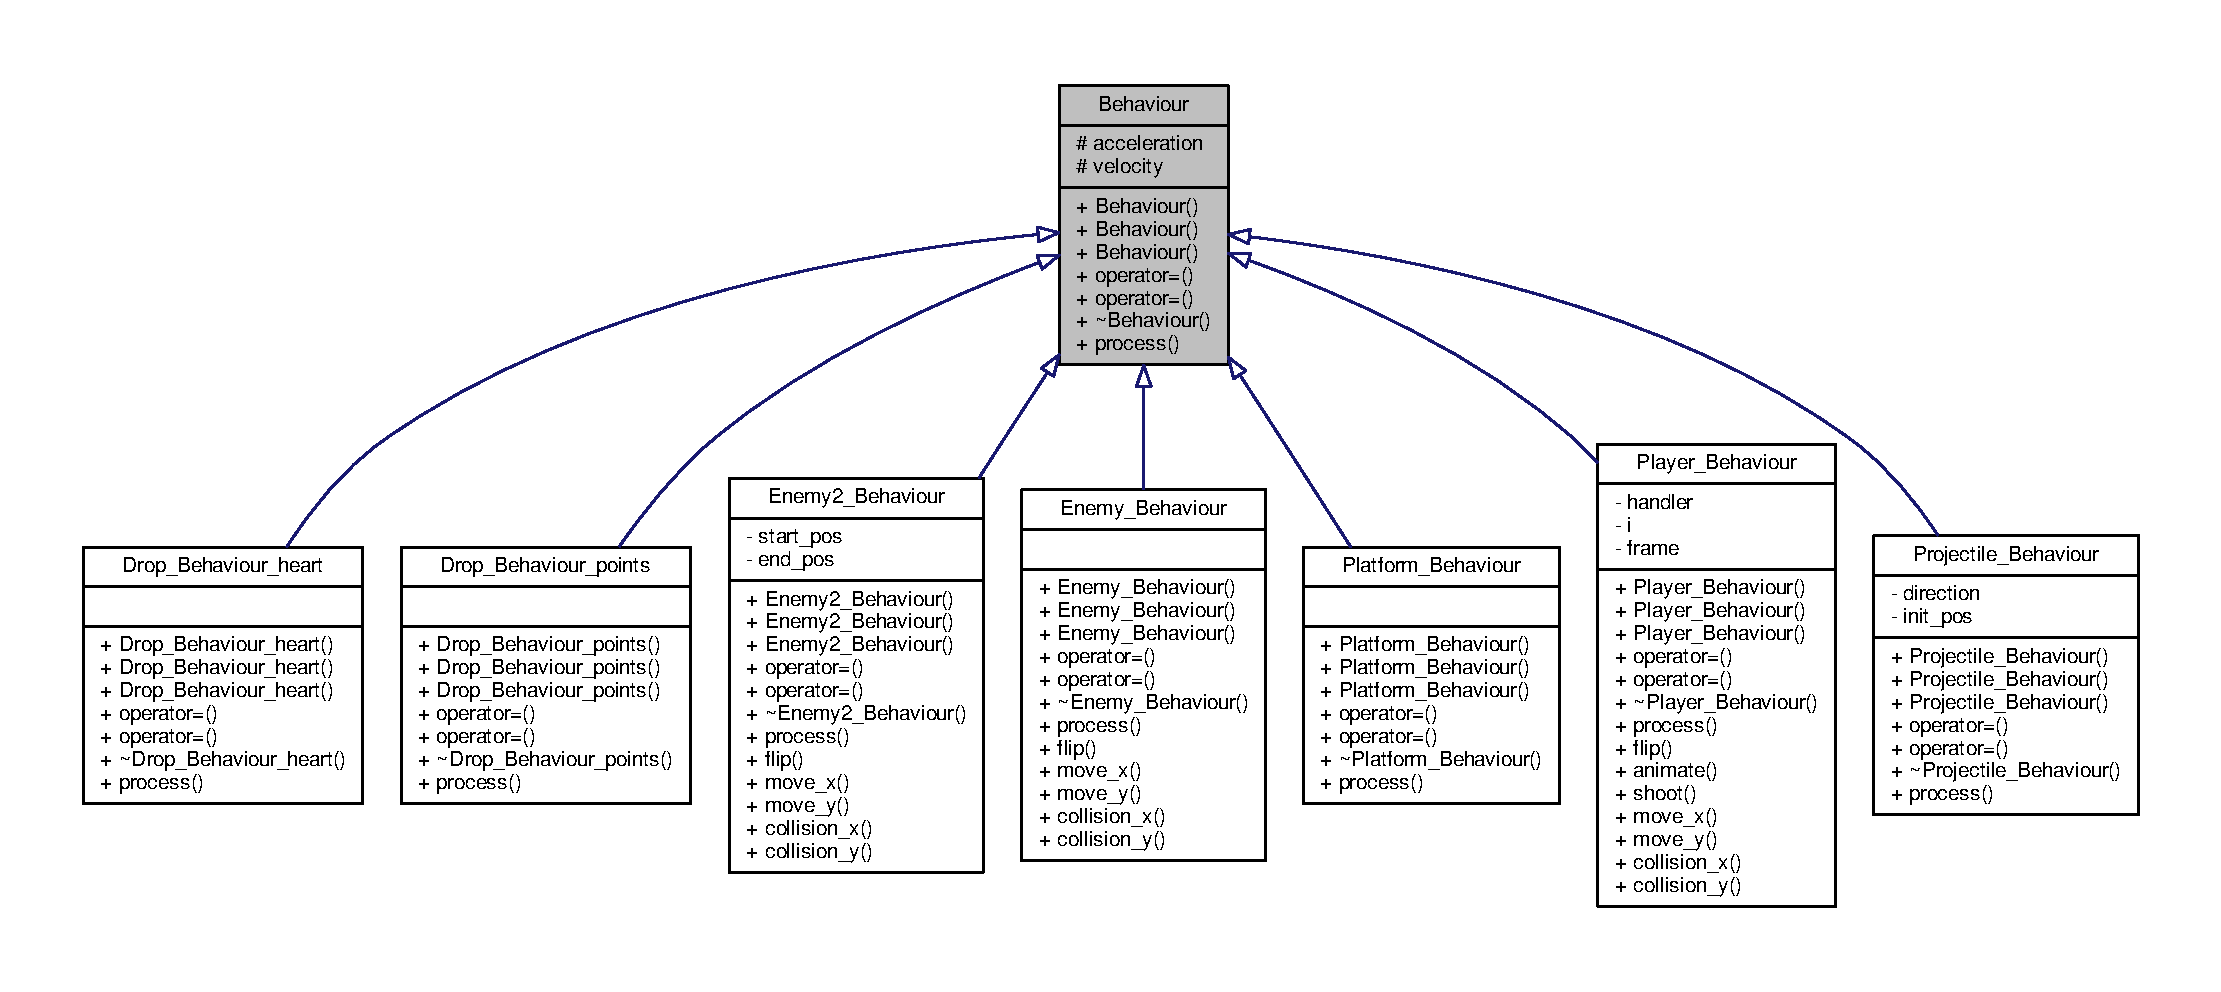
\includegraphics[width=350pt]{classBehaviour__inherit__graph}
\end{center}
\end{figure}


Collaboration diagram for Behaviour\+:\nopagebreak
\begin{figure}[H]
\begin{center}
\leavevmode
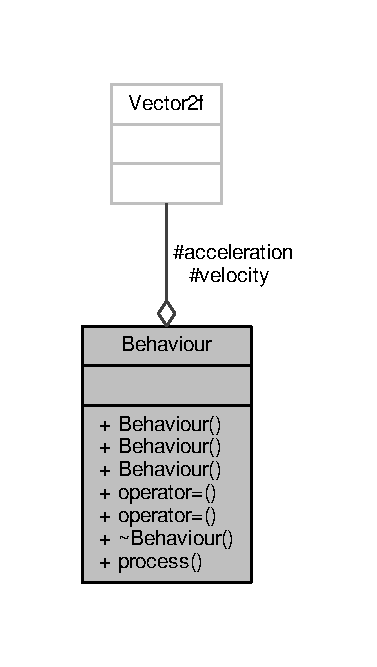
\includegraphics[width=181pt]{classBehaviour__coll__graph}
\end{center}
\end{figure}
\subsection*{Public Member Functions}
\begin{DoxyCompactItemize}
\item 
\hyperlink{classBehaviour_a57e050961bc1305993adaeac62658657}{Behaviour} ()=default
\begin{DoxyCompactList}\small\item\em Konstruktor som inte tar in något speciellt. \end{DoxyCompactList}\item 
\hyperlink{classBehaviour_a0a4eeb61f67cc58c720a110ef9695a73}{Behaviour} (\hyperlink{classBehaviour}{Behaviour} const \&other)=delete
\begin{DoxyCompactList}\small\item\em Copy konstruktor. \end{DoxyCompactList}\item 
\hyperlink{classBehaviour_ae157e7d158e19b515eaac6ef3b37ef0a}{Behaviour} (\hyperlink{classBehaviour}{Behaviour} \&\&other)=delete
\begin{DoxyCompactList}\small\item\em Move konstruktor. \end{DoxyCompactList}\item 
\hyperlink{classBehaviour}{Behaviour} \& \hyperlink{classBehaviour_a3c0ca3a4544e6c126ddaf662538b2e48}{operator=} (\hyperlink{classBehaviour}{Behaviour} const \&rhs)\&=delete
\begin{DoxyCompactList}\small\item\em Copy operator. \end{DoxyCompactList}\item 
\hyperlink{classBehaviour}{Behaviour} \& \hyperlink{classBehaviour_a1bfe3e24e2776f887cf67863630e4154}{operator=} (\hyperlink{classBehaviour}{Behaviour} \&\&rhs)=delete
\begin{DoxyCompactList}\small\item\em Move operator. \end{DoxyCompactList}\item 
virtual \hyperlink{classBehaviour_a3c695554c881998c9ef87cb407b4e451}{$\sim$\+Behaviour} ()=default
\begin{DoxyCompactList}\small\item\em Virtuell destruktor. \end{DoxyCompactList}\item 
virtual void \hyperlink{classBehaviour_aaa6b4ee24dc3cc546fa4dbb7ba4d20da}{process} (\hyperlink{classWorld}{World} \&, \hyperlink{classEntity}{Entity} \&, sf\+::\+Time const \&)=0
\end{DoxyCompactItemize}
\subsection*{Protected Attributes}
\begin{DoxyCompactItemize}
\item 
sf\+::\+Vector2f \hyperlink{classBehaviour_ac17cf81ceee6a44e8a8ec6ee810c9fd3}{acceleration} \{0.\+0f, 0.\+1f\}
\begin{DoxyCompactList}\small\item\em Variabel för gravitation. \end{DoxyCompactList}\item 
sf\+::\+Vector2f \hyperlink{classBehaviour_a1d52096cf20a59890f7705acbaccf88a}{velocity} \{0.\+0f,0.\+0f\}
\begin{DoxyCompactList}\small\item\em Variabel for hastigheten för entiteten. \end{DoxyCompactList}\end{DoxyCompactItemize}


\subsection{Detailed Description}
\hyperlink{classBehaviour}{Behaviour} ärver ej av någonting och används för att definiera hur ett objekt beter sig i spelvärlden. 

\hyperlink{classBehaviour}{Behaviour} är en abstrakt klass som innehåller grundfunktionerna för alla beteende klasser i projektet. 

\subsection{Constructor \& Destructor Documentation}
\hypertarget{classBehaviour_a57e050961bc1305993adaeac62658657}{\index{Behaviour@{Behaviour}!Behaviour@{Behaviour}}
\index{Behaviour@{Behaviour}!Behaviour@{Behaviour}}
\subsubsection[{Behaviour}]{\setlength{\rightskip}{0pt plus 5cm}Behaviour\+::\+Behaviour (
\begin{DoxyParamCaption}
{}
\end{DoxyParamCaption}
)\hspace{0.3cm}{\ttfamily [default]}}}\label{classBehaviour_a57e050961bc1305993adaeac62658657}


Konstruktor som inte tar in något speciellt. 

\hypertarget{classBehaviour_a0a4eeb61f67cc58c720a110ef9695a73}{\index{Behaviour@{Behaviour}!Behaviour@{Behaviour}}
\index{Behaviour@{Behaviour}!Behaviour@{Behaviour}}
\subsubsection[{Behaviour}]{\setlength{\rightskip}{0pt plus 5cm}Behaviour\+::\+Behaviour (
\begin{DoxyParamCaption}
\item[{{\bf Behaviour} const \&}]{other}
\end{DoxyParamCaption}
)\hspace{0.3cm}{\ttfamily [delete]}}}\label{classBehaviour_a0a4eeb61f67cc58c720a110ef9695a73}


Copy konstruktor. 

\hypertarget{classBehaviour_ae157e7d158e19b515eaac6ef3b37ef0a}{\index{Behaviour@{Behaviour}!Behaviour@{Behaviour}}
\index{Behaviour@{Behaviour}!Behaviour@{Behaviour}}
\subsubsection[{Behaviour}]{\setlength{\rightskip}{0pt plus 5cm}Behaviour\+::\+Behaviour (
\begin{DoxyParamCaption}
\item[{{\bf Behaviour} \&\&}]{other}
\end{DoxyParamCaption}
)\hspace{0.3cm}{\ttfamily [delete]}}}\label{classBehaviour_ae157e7d158e19b515eaac6ef3b37ef0a}


Move konstruktor. 

\hypertarget{classBehaviour_a3c695554c881998c9ef87cb407b4e451}{\index{Behaviour@{Behaviour}!````~Behaviour@{$\sim$\+Behaviour}}
\index{````~Behaviour@{$\sim$\+Behaviour}!Behaviour@{Behaviour}}
\subsubsection[{$\sim$\+Behaviour}]{\setlength{\rightskip}{0pt plus 5cm}virtual Behaviour\+::$\sim$\+Behaviour (
\begin{DoxyParamCaption}
{}
\end{DoxyParamCaption}
)\hspace{0.3cm}{\ttfamily [virtual]}, {\ttfamily [default]}}}\label{classBehaviour_a3c695554c881998c9ef87cb407b4e451}


Virtuell destruktor. 



\subsection{Member Function Documentation}
\hypertarget{classBehaviour_a3c0ca3a4544e6c126ddaf662538b2e48}{\index{Behaviour@{Behaviour}!operator=@{operator=}}
\index{operator=@{operator=}!Behaviour@{Behaviour}}
\subsubsection[{operator=}]{\setlength{\rightskip}{0pt plus 5cm}{\bf Behaviour}\& Behaviour\+::operator= (
\begin{DoxyParamCaption}
\item[{{\bf Behaviour} const \&}]{rhs}
\end{DoxyParamCaption}
)\hspace{0.3cm}{\ttfamily [delete]}}}\label{classBehaviour_a3c0ca3a4544e6c126ddaf662538b2e48}


Copy operator. 

\hypertarget{classBehaviour_a1bfe3e24e2776f887cf67863630e4154}{\index{Behaviour@{Behaviour}!operator=@{operator=}}
\index{operator=@{operator=}!Behaviour@{Behaviour}}
\subsubsection[{operator=}]{\setlength{\rightskip}{0pt plus 5cm}{\bf Behaviour}\& Behaviour\+::operator= (
\begin{DoxyParamCaption}
\item[{{\bf Behaviour} \&\&}]{rhs}
\end{DoxyParamCaption}
)\hspace{0.3cm}{\ttfamily [delete]}}}\label{classBehaviour_a1bfe3e24e2776f887cf67863630e4154}


Move operator. 

\hypertarget{classBehaviour_aaa6b4ee24dc3cc546fa4dbb7ba4d20da}{\index{Behaviour@{Behaviour}!process@{process}}
\index{process@{process}!Behaviour@{Behaviour}}
\subsubsection[{process}]{\setlength{\rightskip}{0pt plus 5cm}virtual void Behaviour\+::process (
\begin{DoxyParamCaption}
\item[{{\bf World} \&}]{, }
\item[{{\bf Entity} \&}]{, }
\item[{sf\+::\+Time const \&}]{}
\end{DoxyParamCaption}
)\hspace{0.3cm}{\ttfamily [pure virtual]}}}\label{classBehaviour_aaa6b4ee24dc3cc546fa4dbb7ba4d20da}
Virtuell funktion där själva beteendet händer. Tar in spelvärlden, ägaren till beteendet och tiden sen senaste uppdateringen. 

Implemented in \hyperlink{classPlayer__Behaviour_aa88f449e71197691e1166e985f165fa6}{Player\+\_\+\+Behaviour}, \hyperlink{classEnemy2__Behaviour_a0979bade3f9b3ff9dca3c6b970a5ef63}{Enemy2\+\_\+\+Behaviour}, \hyperlink{classEnemy__Behaviour_a19097e215910b3fd8cf9e002a6f7f642}{Enemy\+\_\+\+Behaviour}, \hyperlink{classProjectile__Behaviour_aed04c8c1f5ae6aca08bdf05b6248d24a}{Projectile\+\_\+\+Behaviour}, \hyperlink{classDrop__Behaviour__heart_a38a5d26b313a84e4428093d537a446fb}{Drop\+\_\+\+Behaviour\+\_\+heart}, \hyperlink{classPlatform__Behaviour_a8a1b458d89bca1e1955aebc2fb44d052}{Platform\+\_\+\+Behaviour}, and \hyperlink{classDrop__Behaviour__points_a37b589ed4fe56c64b1c1b0bf3605e4ba}{Drop\+\_\+\+Behaviour\+\_\+points}.



\subsection{Member Data Documentation}
\hypertarget{classBehaviour_ac17cf81ceee6a44e8a8ec6ee810c9fd3}{\index{Behaviour@{Behaviour}!acceleration@{acceleration}}
\index{acceleration@{acceleration}!Behaviour@{Behaviour}}
\subsubsection[{acceleration}]{\setlength{\rightskip}{0pt plus 5cm}sf\+::\+Vector2f Behaviour\+::acceleration \{0.\+0f, 0.\+1f\}\hspace{0.3cm}{\ttfamily [protected]}}}\label{classBehaviour_ac17cf81ceee6a44e8a8ec6ee810c9fd3}


Variabel för gravitation. 

\hypertarget{classBehaviour_a1d52096cf20a59890f7705acbaccf88a}{\index{Behaviour@{Behaviour}!velocity@{velocity}}
\index{velocity@{velocity}!Behaviour@{Behaviour}}
\subsubsection[{velocity}]{\setlength{\rightskip}{0pt plus 5cm}sf\+::\+Vector2f Behaviour\+::velocity \{0.\+0f,0.\+0f\}\hspace{0.3cm}{\ttfamily [protected]}}}\label{classBehaviour_a1d52096cf20a59890f7705acbaccf88a}


Variabel for hastigheten för entiteten. 



The documentation for this class was generated from the following file\+:\begin{DoxyCompactItemize}
\item 
source/objects/headers/Behaviour.\+h\end{DoxyCompactItemize}

\hypertarget{classDrop}{\section{Drop Class Reference}
\label{classDrop}\index{Drop@{Drop}}
}


\hyperlink{classDrop}{Drop} ärver från \hyperlink{classEntity}{Entity} och innehåller all information för en entitet av droptyp.  




{\ttfamily \#include $<$Drop.\+h$>$}



Inheritance diagram for Drop\+:\nopagebreak
\begin{figure}[H]
\begin{center}
\leavevmode
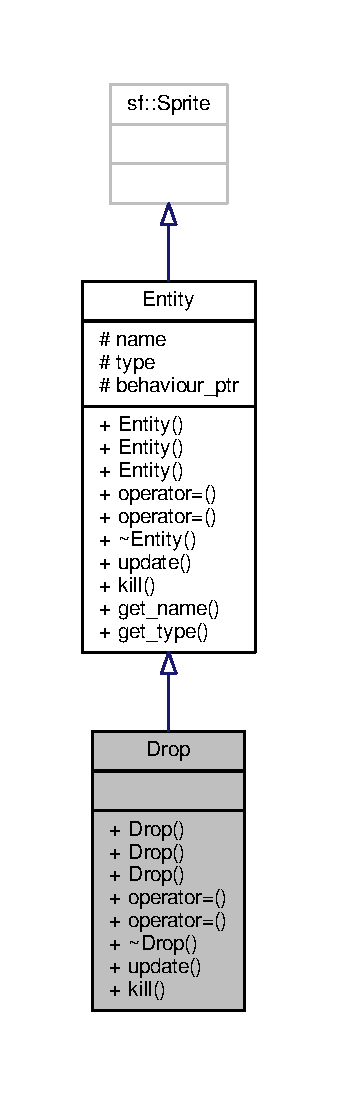
\includegraphics[width=162pt]{classDrop__inherit__graph}
\end{center}
\end{figure}


Collaboration diagram for Drop\+:\nopagebreak
\begin{figure}[H]
\begin{center}
\leavevmode
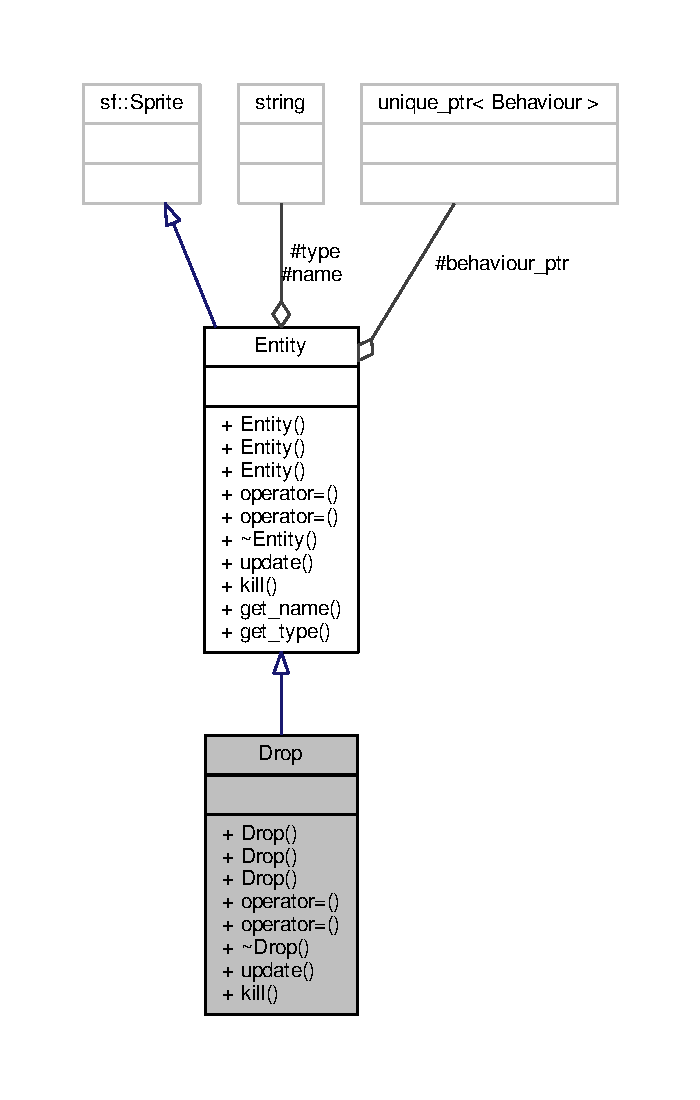
\includegraphics[width=336pt]{classDrop__coll__graph}
\end{center}
\end{figure}
\subsection*{Public Member Functions}
\begin{DoxyCompactItemize}
\item 
\hyperlink{classDrop_a6c26092306a5b47e85bea5db13598e8f}{Drop} (std\+::string, std\+::string, \hyperlink{classBehaviour}{Behaviour} $\ast$, float, float, sf\+::\+Texture const \&, sf\+::\+Int\+Rect)
\item 
\hyperlink{classDrop_ae8d6c72867091cf06b1cc90bd1de1d33}{Drop} (\hyperlink{classDrop}{Drop} const \&other)=delete
\begin{DoxyCompactList}\small\item\em Copy konstruktor. \end{DoxyCompactList}\item 
\hyperlink{classDrop_a073b0384031727ed673f45b8cf9d7a9c}{Drop} (\hyperlink{classDrop}{Drop} \&\&other)=delete
\begin{DoxyCompactList}\small\item\em Move konstruktor. \end{DoxyCompactList}\item 
\hyperlink{classDrop}{Drop} \& \hyperlink{classDrop_a9750d2b430032b1468242fdc59e9f3b4}{operator=} (\hyperlink{classDrop}{Drop} const \&rhs)\&=delete
\begin{DoxyCompactList}\small\item\em Copy operator. \end{DoxyCompactList}\item 
\hyperlink{classDrop}{Drop} \& \hyperlink{classDrop_a033da302213213df357084484b540006}{operator=} (\hyperlink{classDrop}{Drop} \&\&rhs)=delete
\begin{DoxyCompactList}\small\item\em Move operator. \end{DoxyCompactList}\item 
\hyperlink{classDrop_aaa217fe569287d8c9aa27745d545ab87}{$\sim$\+Drop} ()=default
\begin{DoxyCompactList}\small\item\em Default destruktor. \end{DoxyCompactList}\item 
void \hyperlink{classDrop_aa899493774d2a66cbb51f3cd9a0cf80e}{update} (\hyperlink{classWorld}{World} \&, sf\+::\+Time const \&) override
\item 
void \hyperlink{classDrop_a8bbd94b3140a246297aaf4c984dad4ee}{kill} (\hyperlink{classWorld}{World} \&) override
\begin{DoxyCompactList}\small\item\em Om det här objektet har dödats så kommer kill att göra det genom att informera \hyperlink{classWorld}{World} om det. \end{DoxyCompactList}\item 
std\+::string \hyperlink{classEntity_a75c7e4aad3df2e053ee5b43169509534}{get\+\_\+name} () const 
\begin{DoxyCompactList}\small\item\em Returnerar namnet på entititen. \end{DoxyCompactList}\item 
std\+::string \hyperlink{classEntity_a0e9ef479c1147e21e5bcb338cb858df2}{get\+\_\+type} () const 
\begin{DoxyCompactList}\small\item\em Returnerar typen på entititen. \end{DoxyCompactList}\end{DoxyCompactItemize}
\subsection*{Protected Attributes}
\begin{DoxyCompactItemize}
\item 
std\+::string \hyperlink{classEntity_a931b21fbdebb1a5963b4bcab5df128f5}{name}
\begin{DoxyCompactList}\small\item\em Namn. \end{DoxyCompactList}\item 
std\+::string \hyperlink{classEntity_a298a9ebf2474bb00874b5ff6a0d637ef}{type}
\begin{DoxyCompactList}\small\item\em Typ. \end{DoxyCompactList}\item 
std\+::unique\+\_\+ptr$<$ \hyperlink{classBehaviour}{Behaviour} $>$ \hyperlink{classEntity_adb6e36848db24e6d48e6d295e19d3972}{behaviour\+\_\+ptr}
\begin{DoxyCompactList}\small\item\em Unik smart-\/pekare till ett objekt av \hyperlink{classBehaviour}{Behaviour} klassen. \end{DoxyCompactList}\end{DoxyCompactItemize}


\subsection{Detailed Description}
\hyperlink{classDrop}{Drop} ärver från \hyperlink{classEntity}{Entity} och innehåller all information för en entitet av droptyp. 

\hyperlink{classDrop}{Drop} ärver från den abstrakta klassen \hyperlink{classEntity}{Entity} och däför behöver den köra override på \hyperlink{classDrop_aa899493774d2a66cbb51f3cd9a0cf80e}{update()} och Kill(). Den innehåller information om drop objekten och agerar bro mellan \hyperlink{classWorld}{World} och Behaviours. 

\subsection{Constructor \& Destructor Documentation}
\hypertarget{classDrop_a6c26092306a5b47e85bea5db13598e8f}{\index{Drop@{Drop}!Drop@{Drop}}
\index{Drop@{Drop}!Drop@{Drop}}
\subsubsection[{Drop}]{\setlength{\rightskip}{0pt plus 5cm}Drop\+::\+Drop (
\begin{DoxyParamCaption}
\item[{std\+::string}]{n, }
\item[{std\+::string}]{t, }
\item[{{\bf Behaviour} $\ast$}]{b, }
\item[{float}]{x, }
\item[{float}]{y, }
\item[{sf\+::\+Texture const \&}]{texture, }
\item[{sf\+::\+Int\+Rect}]{size}
\end{DoxyParamCaption}
)}}\label{classDrop_a6c26092306a5b47e85bea5db13598e8f}
\hyperlink{classDrop}{Drop}'s konstruktor tar in ett namn, en typ, en pekare till ett objekt av Behaviour-\/typ, x och y värdet där objektet ska finnas, en texture från \hyperlink{classTexture__Container}{Texture\+\_\+\+Container} och vilken del av texturen som ska visas \hypertarget{classDrop_ae8d6c72867091cf06b1cc90bd1de1d33}{\index{Drop@{Drop}!Drop@{Drop}}
\index{Drop@{Drop}!Drop@{Drop}}
\subsubsection[{Drop}]{\setlength{\rightskip}{0pt plus 5cm}Drop\+::\+Drop (
\begin{DoxyParamCaption}
\item[{{\bf Drop} const \&}]{other}
\end{DoxyParamCaption}
)\hspace{0.3cm}{\ttfamily [delete]}}}\label{classDrop_ae8d6c72867091cf06b1cc90bd1de1d33}


Copy konstruktor. 

\hypertarget{classDrop_a073b0384031727ed673f45b8cf9d7a9c}{\index{Drop@{Drop}!Drop@{Drop}}
\index{Drop@{Drop}!Drop@{Drop}}
\subsubsection[{Drop}]{\setlength{\rightskip}{0pt plus 5cm}Drop\+::\+Drop (
\begin{DoxyParamCaption}
\item[{{\bf Drop} \&\&}]{other}
\end{DoxyParamCaption}
)\hspace{0.3cm}{\ttfamily [delete]}}}\label{classDrop_a073b0384031727ed673f45b8cf9d7a9c}


Move konstruktor. 

\hypertarget{classDrop_aaa217fe569287d8c9aa27745d545ab87}{\index{Drop@{Drop}!````~Drop@{$\sim$\+Drop}}
\index{````~Drop@{$\sim$\+Drop}!Drop@{Drop}}
\subsubsection[{$\sim$\+Drop}]{\setlength{\rightskip}{0pt plus 5cm}Drop\+::$\sim$\+Drop (
\begin{DoxyParamCaption}
{}
\end{DoxyParamCaption}
)\hspace{0.3cm}{\ttfamily [default]}}}\label{classDrop_aaa217fe569287d8c9aa27745d545ab87}


Default destruktor. 



\subsection{Member Function Documentation}
\hypertarget{classEntity_a75c7e4aad3df2e053ee5b43169509534}{\index{Drop@{Drop}!get\+\_\+name@{get\+\_\+name}}
\index{get\+\_\+name@{get\+\_\+name}!Drop@{Drop}}
\subsubsection[{get\+\_\+name}]{\setlength{\rightskip}{0pt plus 5cm}std\+::string Entity\+::get\+\_\+name (
\begin{DoxyParamCaption}
{}
\end{DoxyParamCaption}
) const\hspace{0.3cm}{\ttfamily [inline]}, {\ttfamily [inherited]}}}\label{classEntity_a75c7e4aad3df2e053ee5b43169509534}


Returnerar namnet på entititen. 

\hypertarget{classEntity_a0e9ef479c1147e21e5bcb338cb858df2}{\index{Drop@{Drop}!get\+\_\+type@{get\+\_\+type}}
\index{get\+\_\+type@{get\+\_\+type}!Drop@{Drop}}
\subsubsection[{get\+\_\+type}]{\setlength{\rightskip}{0pt plus 5cm}std\+::string Entity\+::get\+\_\+type (
\begin{DoxyParamCaption}
{}
\end{DoxyParamCaption}
) const\hspace{0.3cm}{\ttfamily [inline]}, {\ttfamily [inherited]}}}\label{classEntity_a0e9ef479c1147e21e5bcb338cb858df2}


Returnerar typen på entititen. 

\hypertarget{classDrop_a8bbd94b3140a246297aaf4c984dad4ee}{\index{Drop@{Drop}!kill@{kill}}
\index{kill@{kill}!Drop@{Drop}}
\subsubsection[{kill}]{\setlength{\rightskip}{0pt plus 5cm}void Drop\+::kill (
\begin{DoxyParamCaption}
\item[{{\bf World} \&}]{w}
\end{DoxyParamCaption}
)\hspace{0.3cm}{\ttfamily [override]}, {\ttfamily [virtual]}}}\label{classDrop_a8bbd94b3140a246297aaf4c984dad4ee}


Om det här objektet har dödats så kommer kill att göra det genom att informera \hyperlink{classWorld}{World} om det. 



Implements \hyperlink{classEntity_a3d585a30d7f07c50911485825f5496cd}{Entity}.

\hypertarget{classDrop_a9750d2b430032b1468242fdc59e9f3b4}{\index{Drop@{Drop}!operator=@{operator=}}
\index{operator=@{operator=}!Drop@{Drop}}
\subsubsection[{operator=}]{\setlength{\rightskip}{0pt plus 5cm}{\bf Drop}\& Drop\+::operator= (
\begin{DoxyParamCaption}
\item[{{\bf Drop} const \&}]{rhs}
\end{DoxyParamCaption}
)\hspace{0.3cm}{\ttfamily [delete]}}}\label{classDrop_a9750d2b430032b1468242fdc59e9f3b4}


Copy operator. 

\hypertarget{classDrop_a033da302213213df357084484b540006}{\index{Drop@{Drop}!operator=@{operator=}}
\index{operator=@{operator=}!Drop@{Drop}}
\subsubsection[{operator=}]{\setlength{\rightskip}{0pt plus 5cm}{\bf Drop}\& Drop\+::operator= (
\begin{DoxyParamCaption}
\item[{{\bf Drop} \&\&}]{rhs}
\end{DoxyParamCaption}
)\hspace{0.3cm}{\ttfamily [delete]}}}\label{classDrop_a033da302213213df357084484b540006}


Move operator. 

\hypertarget{classDrop_aa899493774d2a66cbb51f3cd9a0cf80e}{\index{Drop@{Drop}!update@{update}}
\index{update@{update}!Drop@{Drop}}
\subsubsection[{update}]{\setlength{\rightskip}{0pt plus 5cm}void Drop\+::update (
\begin{DoxyParamCaption}
\item[{{\bf World} \&}]{world, }
\item[{sf\+::\+Time const \&}]{t}
\end{DoxyParamCaption}
)\hspace{0.3cm}{\ttfamily [override]}, {\ttfamily [virtual]}}}\label{classDrop_aa899493774d2a66cbb51f3cd9a0cf80e}
\hyperlink{classEntity_a180102ac6695559b1f8fcf0aee747802}{Entity\+::update()} override Funktion som kallas av world när det här specifika objektet ska uppdatera sig. Det gör sedan detta genom att t.\+ex. flytta på sig och kolla kollisioner. 

Implements \hyperlink{classEntity_a180102ac6695559b1f8fcf0aee747802}{Entity}.



\subsection{Member Data Documentation}
\hypertarget{classEntity_adb6e36848db24e6d48e6d295e19d3972}{\index{Drop@{Drop}!behaviour\+\_\+ptr@{behaviour\+\_\+ptr}}
\index{behaviour\+\_\+ptr@{behaviour\+\_\+ptr}!Drop@{Drop}}
\subsubsection[{behaviour\+\_\+ptr}]{\setlength{\rightskip}{0pt plus 5cm}std\+::unique\+\_\+ptr$<${\bf Behaviour}$>$ Entity\+::behaviour\+\_\+ptr\hspace{0.3cm}{\ttfamily [protected]}, {\ttfamily [inherited]}}}\label{classEntity_adb6e36848db24e6d48e6d295e19d3972}


Unik smart-\/pekare till ett objekt av \hyperlink{classBehaviour}{Behaviour} klassen. 

\hypertarget{classEntity_a931b21fbdebb1a5963b4bcab5df128f5}{\index{Drop@{Drop}!name@{name}}
\index{name@{name}!Drop@{Drop}}
\subsubsection[{name}]{\setlength{\rightskip}{0pt plus 5cm}std\+::string Entity\+::name\hspace{0.3cm}{\ttfamily [protected]}, {\ttfamily [inherited]}}}\label{classEntity_a931b21fbdebb1a5963b4bcab5df128f5}


Namn. 

\hypertarget{classEntity_a298a9ebf2474bb00874b5ff6a0d637ef}{\index{Drop@{Drop}!type@{type}}
\index{type@{type}!Drop@{Drop}}
\subsubsection[{type}]{\setlength{\rightskip}{0pt plus 5cm}std\+::string Entity\+::type\hspace{0.3cm}{\ttfamily [protected]}, {\ttfamily [inherited]}}}\label{classEntity_a298a9ebf2474bb00874b5ff6a0d637ef}


Typ. 



The documentation for this class was generated from the following files\+:\begin{DoxyCompactItemize}
\item 
source/objects/headers/Drop.\+h\item 
source/objects/imps/Drop.\+cpp\end{DoxyCompactItemize}

\hypertarget{classDrop__Behaviour__heart}{\section{Drop\+\_\+\+Behaviour\+\_\+heart Class Reference}
\label{classDrop__Behaviour__heart}\index{Drop\+\_\+\+Behaviour\+\_\+heart@{Drop\+\_\+\+Behaviour\+\_\+heart}}
}


\hyperlink{classDrop__Behaviour__heart}{Drop\+\_\+\+Behaviour\+\_\+heart} ärver från \hyperlink{classBehaviour}{Behaviour} och tillhandahåller beteendet för hjärt-\/drops.  




{\ttfamily \#include $<$Drop\+\_\+\+Behaviour\+\_\+heart.\+h$>$}



Inheritance diagram for Drop\+\_\+\+Behaviour\+\_\+heart\+:\nopagebreak
\begin{figure}[H]
\begin{center}
\leavevmode
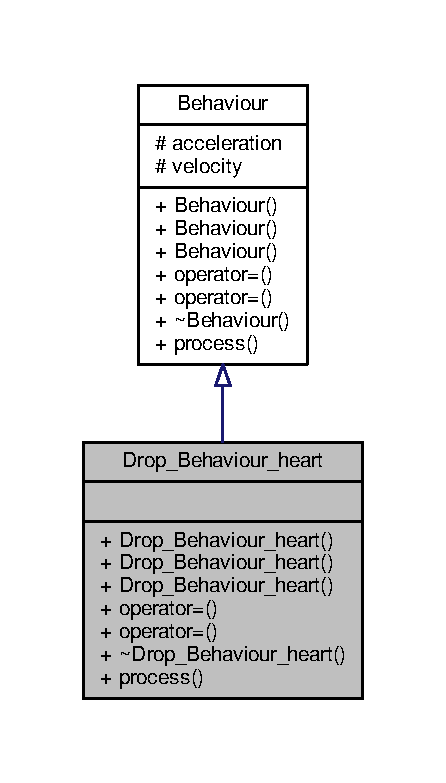
\includegraphics[width=214pt]{classDrop__Behaviour__heart__inherit__graph}
\end{center}
\end{figure}


Collaboration diagram for Drop\+\_\+\+Behaviour\+\_\+heart\+:\nopagebreak
\begin{figure}[H]
\begin{center}
\leavevmode
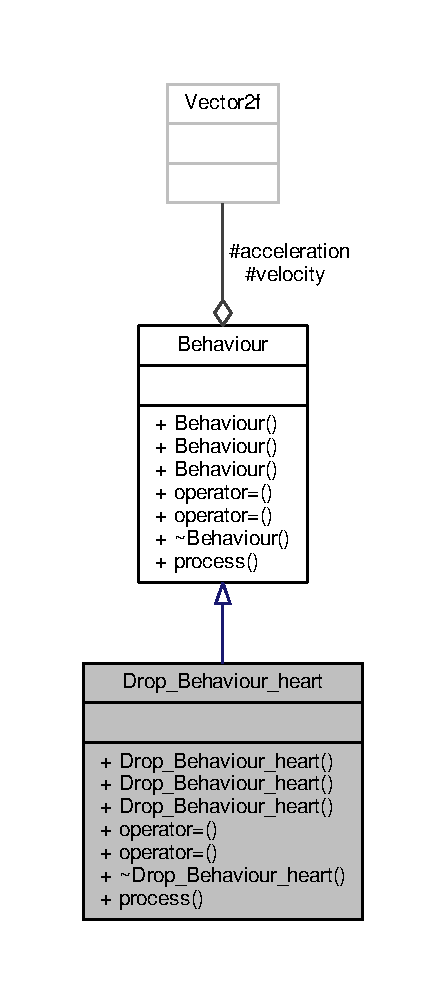
\includegraphics[width=214pt]{classDrop__Behaviour__heart__coll__graph}
\end{center}
\end{figure}
\subsection*{Public Member Functions}
\begin{DoxyCompactItemize}
\item 
\hyperlink{classDrop__Behaviour__heart_ab0778d4ffa9b938005d57f580c8aebf7}{Drop\+\_\+\+Behaviour\+\_\+heart} ()
\begin{DoxyCompactList}\small\item\em Konstruktor som bara använder Behaviours konstruktor. \end{DoxyCompactList}\item 
\hyperlink{classDrop__Behaviour__heart_a8554c784f0215bad588437e37a5674a0}{Drop\+\_\+\+Behaviour\+\_\+heart} (\hyperlink{classDrop__Behaviour__heart}{Drop\+\_\+\+Behaviour\+\_\+heart} const \&other)=delete
\begin{DoxyCompactList}\small\item\em Copy konstruktor. \end{DoxyCompactList}\item 
\hyperlink{classDrop__Behaviour__heart_a782f27c01ccfffeca4e5ee1d793adec7}{Drop\+\_\+\+Behaviour\+\_\+heart} (\hyperlink{classDrop__Behaviour__heart}{Drop\+\_\+\+Behaviour\+\_\+heart} \&\&other)=delete
\begin{DoxyCompactList}\small\item\em Move konstruktor. \end{DoxyCompactList}\item 
\hyperlink{classDrop__Behaviour__heart}{Drop\+\_\+\+Behaviour\+\_\+heart} \& \hyperlink{classDrop__Behaviour__heart_a9fda609e7c9ec29d050e7952e3600674}{operator=} (\hyperlink{classDrop__Behaviour__heart}{Drop\+\_\+\+Behaviour\+\_\+heart} const \&rhs)\&=delete
\begin{DoxyCompactList}\small\item\em Copy operator. \end{DoxyCompactList}\item 
\hyperlink{classDrop__Behaviour__heart}{Drop\+\_\+\+Behaviour\+\_\+heart} \& \hyperlink{classDrop__Behaviour__heart_a8b01d23278f6521ef9374208eda83972}{operator=} (\hyperlink{classDrop__Behaviour__heart}{Drop\+\_\+\+Behaviour\+\_\+heart} \&\&rhs)=delete
\begin{DoxyCompactList}\small\item\em Move operator. \end{DoxyCompactList}\item 
\hyperlink{classDrop__Behaviour__heart_a2f8021b6474c8c010969cc12cd2b8cc1}{$\sim$\+Drop\+\_\+\+Behaviour\+\_\+heart} ()=default
\begin{DoxyCompactList}\small\item\em Default destruktor. \end{DoxyCompactList}\item 
void \hyperlink{classDrop__Behaviour__heart_a38a5d26b313a84e4428093d537a446fb}{process} (\hyperlink{classWorld}{World} \&, \hyperlink{classEntity}{Entity} \&, sf\+::\+Time const \&) override
\begin{DoxyCompactList}\small\item\em Process som låter hjärtat ramla ner, kollidera med platformar och sedan försvinna när det kolliderar med en spelare. \end{DoxyCompactList}\end{DoxyCompactItemize}
\subsection*{Protected Attributes}
\begin{DoxyCompactItemize}
\item 
sf\+::\+Vector2f \hyperlink{classBehaviour_ac17cf81ceee6a44e8a8ec6ee810c9fd3}{acceleration} \{0.\+0f, 0.\+1f\}
\begin{DoxyCompactList}\small\item\em Variabel för gravitation. \end{DoxyCompactList}\item 
sf\+::\+Vector2f \hyperlink{classBehaviour_a1d52096cf20a59890f7705acbaccf88a}{velocity} \{0.\+0f,0.\+0f\}
\begin{DoxyCompactList}\small\item\em Variabel for hastigheten för entiteten. \end{DoxyCompactList}\end{DoxyCompactItemize}


\subsection{Detailed Description}
\hyperlink{classDrop__Behaviour__heart}{Drop\+\_\+\+Behaviour\+\_\+heart} ärver från \hyperlink{classBehaviour}{Behaviour} och tillhandahåller beteendet för hjärt-\/drops. 

\hyperlink{classDrop__Behaviour__heart}{Drop\+\_\+\+Behaviour\+\_\+heart} ärver från de abstrakta klassen \hyperlink{classBehaviour}{Behaviour} och däför behöver den köra override på \hyperlink{classDrop__Behaviour__heart_a38a5d26b313a84e4428093d537a446fb}{process()} 

\subsection{Constructor \& Destructor Documentation}
\hypertarget{classDrop__Behaviour__heart_ab0778d4ffa9b938005d57f580c8aebf7}{\index{Drop\+\_\+\+Behaviour\+\_\+heart@{Drop\+\_\+\+Behaviour\+\_\+heart}!Drop\+\_\+\+Behaviour\+\_\+heart@{Drop\+\_\+\+Behaviour\+\_\+heart}}
\index{Drop\+\_\+\+Behaviour\+\_\+heart@{Drop\+\_\+\+Behaviour\+\_\+heart}!Drop\+\_\+\+Behaviour\+\_\+heart@{Drop\+\_\+\+Behaviour\+\_\+heart}}
\subsubsection[{Drop\+\_\+\+Behaviour\+\_\+heart}]{\setlength{\rightskip}{0pt plus 5cm}Drop\+\_\+\+Behaviour\+\_\+heart\+::\+Drop\+\_\+\+Behaviour\+\_\+heart (
\begin{DoxyParamCaption}
{}
\end{DoxyParamCaption}
)\hspace{0.3cm}{\ttfamily [inline]}}}\label{classDrop__Behaviour__heart_ab0778d4ffa9b938005d57f580c8aebf7}


Konstruktor som bara använder Behaviours konstruktor. 

\hypertarget{classDrop__Behaviour__heart_a8554c784f0215bad588437e37a5674a0}{\index{Drop\+\_\+\+Behaviour\+\_\+heart@{Drop\+\_\+\+Behaviour\+\_\+heart}!Drop\+\_\+\+Behaviour\+\_\+heart@{Drop\+\_\+\+Behaviour\+\_\+heart}}
\index{Drop\+\_\+\+Behaviour\+\_\+heart@{Drop\+\_\+\+Behaviour\+\_\+heart}!Drop\+\_\+\+Behaviour\+\_\+heart@{Drop\+\_\+\+Behaviour\+\_\+heart}}
\subsubsection[{Drop\+\_\+\+Behaviour\+\_\+heart}]{\setlength{\rightskip}{0pt plus 5cm}Drop\+\_\+\+Behaviour\+\_\+heart\+::\+Drop\+\_\+\+Behaviour\+\_\+heart (
\begin{DoxyParamCaption}
\item[{{\bf Drop\+\_\+\+Behaviour\+\_\+heart} const \&}]{other}
\end{DoxyParamCaption}
)\hspace{0.3cm}{\ttfamily [delete]}}}\label{classDrop__Behaviour__heart_a8554c784f0215bad588437e37a5674a0}


Copy konstruktor. 

\hypertarget{classDrop__Behaviour__heart_a782f27c01ccfffeca4e5ee1d793adec7}{\index{Drop\+\_\+\+Behaviour\+\_\+heart@{Drop\+\_\+\+Behaviour\+\_\+heart}!Drop\+\_\+\+Behaviour\+\_\+heart@{Drop\+\_\+\+Behaviour\+\_\+heart}}
\index{Drop\+\_\+\+Behaviour\+\_\+heart@{Drop\+\_\+\+Behaviour\+\_\+heart}!Drop\+\_\+\+Behaviour\+\_\+heart@{Drop\+\_\+\+Behaviour\+\_\+heart}}
\subsubsection[{Drop\+\_\+\+Behaviour\+\_\+heart}]{\setlength{\rightskip}{0pt plus 5cm}Drop\+\_\+\+Behaviour\+\_\+heart\+::\+Drop\+\_\+\+Behaviour\+\_\+heart (
\begin{DoxyParamCaption}
\item[{{\bf Drop\+\_\+\+Behaviour\+\_\+heart} \&\&}]{other}
\end{DoxyParamCaption}
)\hspace{0.3cm}{\ttfamily [delete]}}}\label{classDrop__Behaviour__heart_a782f27c01ccfffeca4e5ee1d793adec7}


Move konstruktor. 

\hypertarget{classDrop__Behaviour__heart_a2f8021b6474c8c010969cc12cd2b8cc1}{\index{Drop\+\_\+\+Behaviour\+\_\+heart@{Drop\+\_\+\+Behaviour\+\_\+heart}!````~Drop\+\_\+\+Behaviour\+\_\+heart@{$\sim$\+Drop\+\_\+\+Behaviour\+\_\+heart}}
\index{````~Drop\+\_\+\+Behaviour\+\_\+heart@{$\sim$\+Drop\+\_\+\+Behaviour\+\_\+heart}!Drop\+\_\+\+Behaviour\+\_\+heart@{Drop\+\_\+\+Behaviour\+\_\+heart}}
\subsubsection[{$\sim$\+Drop\+\_\+\+Behaviour\+\_\+heart}]{\setlength{\rightskip}{0pt plus 5cm}Drop\+\_\+\+Behaviour\+\_\+heart\+::$\sim$\+Drop\+\_\+\+Behaviour\+\_\+heart (
\begin{DoxyParamCaption}
{}
\end{DoxyParamCaption}
)\hspace{0.3cm}{\ttfamily [default]}}}\label{classDrop__Behaviour__heart_a2f8021b6474c8c010969cc12cd2b8cc1}


Default destruktor. 



\subsection{Member Function Documentation}
\hypertarget{classDrop__Behaviour__heart_a9fda609e7c9ec29d050e7952e3600674}{\index{Drop\+\_\+\+Behaviour\+\_\+heart@{Drop\+\_\+\+Behaviour\+\_\+heart}!operator=@{operator=}}
\index{operator=@{operator=}!Drop\+\_\+\+Behaviour\+\_\+heart@{Drop\+\_\+\+Behaviour\+\_\+heart}}
\subsubsection[{operator=}]{\setlength{\rightskip}{0pt plus 5cm}{\bf Drop\+\_\+\+Behaviour\+\_\+heart}\& Drop\+\_\+\+Behaviour\+\_\+heart\+::operator= (
\begin{DoxyParamCaption}
\item[{{\bf Drop\+\_\+\+Behaviour\+\_\+heart} const \&}]{rhs}
\end{DoxyParamCaption}
)\hspace{0.3cm}{\ttfamily [delete]}}}\label{classDrop__Behaviour__heart_a9fda609e7c9ec29d050e7952e3600674}


Copy operator. 

\hypertarget{classDrop__Behaviour__heart_a8b01d23278f6521ef9374208eda83972}{\index{Drop\+\_\+\+Behaviour\+\_\+heart@{Drop\+\_\+\+Behaviour\+\_\+heart}!operator=@{operator=}}
\index{operator=@{operator=}!Drop\+\_\+\+Behaviour\+\_\+heart@{Drop\+\_\+\+Behaviour\+\_\+heart}}
\subsubsection[{operator=}]{\setlength{\rightskip}{0pt plus 5cm}{\bf Drop\+\_\+\+Behaviour\+\_\+heart}\& Drop\+\_\+\+Behaviour\+\_\+heart\+::operator= (
\begin{DoxyParamCaption}
\item[{{\bf Drop\+\_\+\+Behaviour\+\_\+heart} \&\&}]{rhs}
\end{DoxyParamCaption}
)\hspace{0.3cm}{\ttfamily [delete]}}}\label{classDrop__Behaviour__heart_a8b01d23278f6521ef9374208eda83972}


Move operator. 

\hypertarget{classDrop__Behaviour__heart_a38a5d26b313a84e4428093d537a446fb}{\index{Drop\+\_\+\+Behaviour\+\_\+heart@{Drop\+\_\+\+Behaviour\+\_\+heart}!process@{process}}
\index{process@{process}!Drop\+\_\+\+Behaviour\+\_\+heart@{Drop\+\_\+\+Behaviour\+\_\+heart}}
\subsubsection[{process}]{\setlength{\rightskip}{0pt plus 5cm}void Drop\+\_\+\+Behaviour\+\_\+heart\+::process (
\begin{DoxyParamCaption}
\item[{{\bf World} \&}]{world, }
\item[{{\bf Entity} \&}]{owner, }
\item[{sf\+::\+Time const \&}]{t}
\end{DoxyParamCaption}
)\hspace{0.3cm}{\ttfamily [override]}, {\ttfamily [virtual]}}}\label{classDrop__Behaviour__heart_a38a5d26b313a84e4428093d537a446fb}


Process som låter hjärtat ramla ner, kollidera med platformar och sedan försvinna när det kolliderar med en spelare. 



Implements \hyperlink{classBehaviour_aaa6b4ee24dc3cc546fa4dbb7ba4d20da}{Behaviour}.



\subsection{Member Data Documentation}
\hypertarget{classBehaviour_ac17cf81ceee6a44e8a8ec6ee810c9fd3}{\index{Drop\+\_\+\+Behaviour\+\_\+heart@{Drop\+\_\+\+Behaviour\+\_\+heart}!acceleration@{acceleration}}
\index{acceleration@{acceleration}!Drop\+\_\+\+Behaviour\+\_\+heart@{Drop\+\_\+\+Behaviour\+\_\+heart}}
\subsubsection[{acceleration}]{\setlength{\rightskip}{0pt plus 5cm}sf\+::\+Vector2f Behaviour\+::acceleration \{0.\+0f, 0.\+1f\}\hspace{0.3cm}{\ttfamily [protected]}, {\ttfamily [inherited]}}}\label{classBehaviour_ac17cf81ceee6a44e8a8ec6ee810c9fd3}


Variabel för gravitation. 

\hypertarget{classBehaviour_a1d52096cf20a59890f7705acbaccf88a}{\index{Drop\+\_\+\+Behaviour\+\_\+heart@{Drop\+\_\+\+Behaviour\+\_\+heart}!velocity@{velocity}}
\index{velocity@{velocity}!Drop\+\_\+\+Behaviour\+\_\+heart@{Drop\+\_\+\+Behaviour\+\_\+heart}}
\subsubsection[{velocity}]{\setlength{\rightskip}{0pt plus 5cm}sf\+::\+Vector2f Behaviour\+::velocity \{0.\+0f,0.\+0f\}\hspace{0.3cm}{\ttfamily [protected]}, {\ttfamily [inherited]}}}\label{classBehaviour_a1d52096cf20a59890f7705acbaccf88a}


Variabel for hastigheten för entiteten. 



The documentation for this class was generated from the following files\+:\begin{DoxyCompactItemize}
\item 
source/objects/headers/Drop\+\_\+\+Behaviour\+\_\+heart.\+h\item 
source/objects/imps/Drop\+\_\+\+Behaviour\+\_\+heart.\+cpp\end{DoxyCompactItemize}

\hypertarget{classDrop__Behaviour__points}{\section{Drop\+\_\+\+Behaviour\+\_\+points Class Reference}
\label{classDrop__Behaviour__points}\index{Drop\+\_\+\+Behaviour\+\_\+points@{Drop\+\_\+\+Behaviour\+\_\+points}}
}


\hyperlink{classDrop__Behaviour__points}{Drop\+\_\+\+Behaviour\+\_\+points} ärver från \hyperlink{classBehaviour}{Behaviour} och tillhandahåller beteendet för poäng-\/drops.  




{\ttfamily \#include $<$Drop\+\_\+\+Behaviour\+\_\+points.\+h$>$}



Inheritance diagram for Drop\+\_\+\+Behaviour\+\_\+points\+:\nopagebreak
\begin{figure}[H]
\begin{center}
\leavevmode
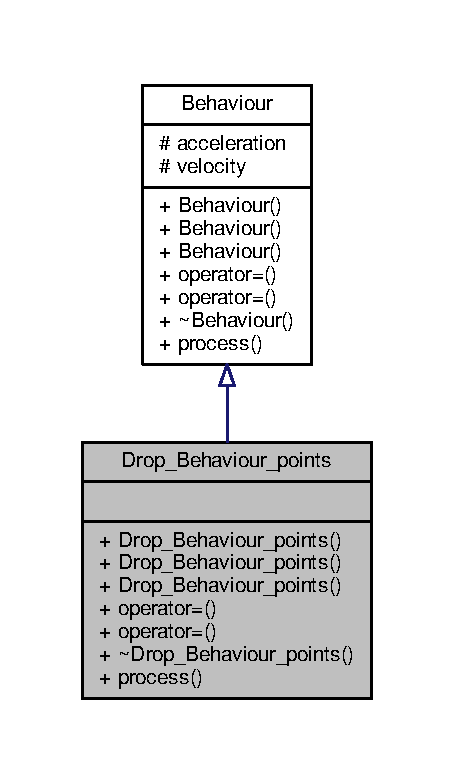
\includegraphics[width=218pt]{classDrop__Behaviour__points__inherit__graph}
\end{center}
\end{figure}


Collaboration diagram for Drop\+\_\+\+Behaviour\+\_\+points\+:\nopagebreak
\begin{figure}[H]
\begin{center}
\leavevmode
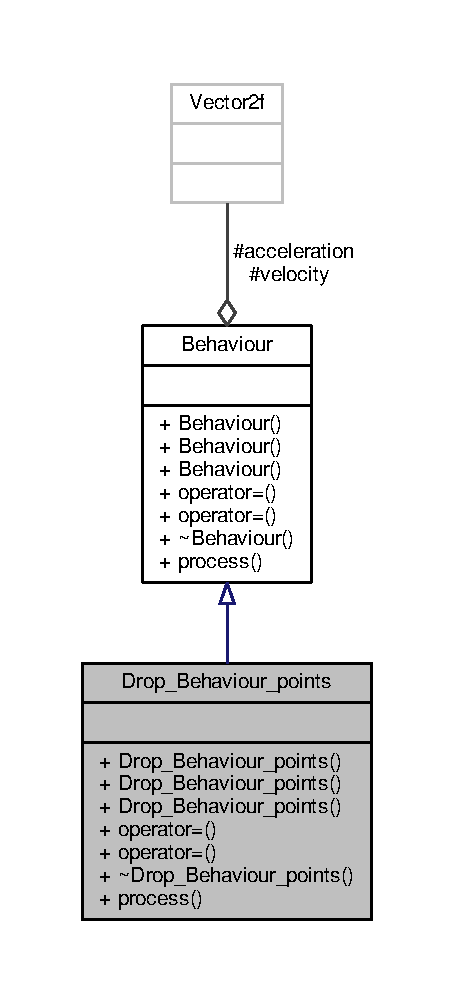
\includegraphics[width=218pt]{classDrop__Behaviour__points__coll__graph}
\end{center}
\end{figure}
\subsection*{Public Member Functions}
\begin{DoxyCompactItemize}
\item 
\hyperlink{classDrop__Behaviour__points_ae0b8b577c979496468672b00605d7793}{Drop\+\_\+\+Behaviour\+\_\+points} ()
\begin{DoxyCompactList}\small\item\em Konstruktor som bara använder Behaviours konstruktor. \end{DoxyCompactList}\item 
\hyperlink{classDrop__Behaviour__points_a17e6caa1f56c5d86db89dbfeed049b3d}{Drop\+\_\+\+Behaviour\+\_\+points} (\hyperlink{classDrop__Behaviour__points}{Drop\+\_\+\+Behaviour\+\_\+points} const \&other)=delete
\begin{DoxyCompactList}\small\item\em Copy konstruktor. \end{DoxyCompactList}\item 
\hyperlink{classDrop__Behaviour__points_a90b77f3562e551e7784eb4c11867757e}{Drop\+\_\+\+Behaviour\+\_\+points} (\hyperlink{classDrop__Behaviour__points}{Drop\+\_\+\+Behaviour\+\_\+points} \&\&other)=delete
\begin{DoxyCompactList}\small\item\em Move konstruktor. \end{DoxyCompactList}\item 
\hyperlink{classDrop__Behaviour__points}{Drop\+\_\+\+Behaviour\+\_\+points} \& \hyperlink{classDrop__Behaviour__points_a016d4fc804706e2230985db16a883d57}{operator=} (\hyperlink{classDrop__Behaviour__points}{Drop\+\_\+\+Behaviour\+\_\+points} const \&rhs)\&=delete
\begin{DoxyCompactList}\small\item\em Copy operator. \end{DoxyCompactList}\item 
\hyperlink{classDrop__Behaviour__points}{Drop\+\_\+\+Behaviour\+\_\+points} \& \hyperlink{classDrop__Behaviour__points_ac8de5ddd7d5e51b56bc133ef1068673f}{operator=} (\hyperlink{classDrop__Behaviour__points}{Drop\+\_\+\+Behaviour\+\_\+points} \&\&rhs)=delete
\begin{DoxyCompactList}\small\item\em Move operator. \end{DoxyCompactList}\item 
\hyperlink{classDrop__Behaviour__points_a8522792b10aebe9d01dd84e87d42baad}{$\sim$\+Drop\+\_\+\+Behaviour\+\_\+points} ()=default
\begin{DoxyCompactList}\small\item\em Default destruktor. \end{DoxyCompactList}\item 
void \hyperlink{classDrop__Behaviour__points_a37b589ed4fe56c64b1c1b0bf3605e4ba}{process} (\hyperlink{classWorld}{World} \&, \hyperlink{classEntity}{Entity} \&, sf\+::\+Time const \&) override
\begin{DoxyCompactList}\small\item\em Process som låter hjärtat ramla ner, kollidera med platformar och sedan försvinna när det kolliderar med en spelare. \end{DoxyCompactList}\end{DoxyCompactItemize}
\subsection*{Protected Attributes}
\begin{DoxyCompactItemize}
\item 
sf\+::\+Vector2f \hyperlink{classBehaviour_ac17cf81ceee6a44e8a8ec6ee810c9fd3}{acceleration} \{0.\+0f, 0.\+1f\}
\begin{DoxyCompactList}\small\item\em Variabel för gravitation. \end{DoxyCompactList}\item 
sf\+::\+Vector2f \hyperlink{classBehaviour_a1d52096cf20a59890f7705acbaccf88a}{velocity} \{0.\+0f,0.\+0f\}
\begin{DoxyCompactList}\small\item\em Variabel for hastigheten för entiteten. \end{DoxyCompactList}\end{DoxyCompactItemize}


\subsection{Detailed Description}
\hyperlink{classDrop__Behaviour__points}{Drop\+\_\+\+Behaviour\+\_\+points} ärver från \hyperlink{classBehaviour}{Behaviour} och tillhandahåller beteendet för poäng-\/drops. 

\hyperlink{classDrop__Behaviour__heart}{Drop\+\_\+\+Behaviour\+\_\+heart} ärver från de abstrakta klassen \hyperlink{classBehaviour}{Behaviour} och däför behöver den köra override på \hyperlink{classDrop__Behaviour__points_a37b589ed4fe56c64b1c1b0bf3605e4ba}{process()} 

\subsection{Constructor \& Destructor Documentation}
\hypertarget{classDrop__Behaviour__points_ae0b8b577c979496468672b00605d7793}{\index{Drop\+\_\+\+Behaviour\+\_\+points@{Drop\+\_\+\+Behaviour\+\_\+points}!Drop\+\_\+\+Behaviour\+\_\+points@{Drop\+\_\+\+Behaviour\+\_\+points}}
\index{Drop\+\_\+\+Behaviour\+\_\+points@{Drop\+\_\+\+Behaviour\+\_\+points}!Drop\+\_\+\+Behaviour\+\_\+points@{Drop\+\_\+\+Behaviour\+\_\+points}}
\subsubsection[{Drop\+\_\+\+Behaviour\+\_\+points}]{\setlength{\rightskip}{0pt plus 5cm}Drop\+\_\+\+Behaviour\+\_\+points\+::\+Drop\+\_\+\+Behaviour\+\_\+points (
\begin{DoxyParamCaption}
{}
\end{DoxyParamCaption}
)\hspace{0.3cm}{\ttfamily [inline]}}}\label{classDrop__Behaviour__points_ae0b8b577c979496468672b00605d7793}


Konstruktor som bara använder Behaviours konstruktor. 

\hypertarget{classDrop__Behaviour__points_a17e6caa1f56c5d86db89dbfeed049b3d}{\index{Drop\+\_\+\+Behaviour\+\_\+points@{Drop\+\_\+\+Behaviour\+\_\+points}!Drop\+\_\+\+Behaviour\+\_\+points@{Drop\+\_\+\+Behaviour\+\_\+points}}
\index{Drop\+\_\+\+Behaviour\+\_\+points@{Drop\+\_\+\+Behaviour\+\_\+points}!Drop\+\_\+\+Behaviour\+\_\+points@{Drop\+\_\+\+Behaviour\+\_\+points}}
\subsubsection[{Drop\+\_\+\+Behaviour\+\_\+points}]{\setlength{\rightskip}{0pt plus 5cm}Drop\+\_\+\+Behaviour\+\_\+points\+::\+Drop\+\_\+\+Behaviour\+\_\+points (
\begin{DoxyParamCaption}
\item[{{\bf Drop\+\_\+\+Behaviour\+\_\+points} const \&}]{other}
\end{DoxyParamCaption}
)\hspace{0.3cm}{\ttfamily [delete]}}}\label{classDrop__Behaviour__points_a17e6caa1f56c5d86db89dbfeed049b3d}


Copy konstruktor. 

\hypertarget{classDrop__Behaviour__points_a90b77f3562e551e7784eb4c11867757e}{\index{Drop\+\_\+\+Behaviour\+\_\+points@{Drop\+\_\+\+Behaviour\+\_\+points}!Drop\+\_\+\+Behaviour\+\_\+points@{Drop\+\_\+\+Behaviour\+\_\+points}}
\index{Drop\+\_\+\+Behaviour\+\_\+points@{Drop\+\_\+\+Behaviour\+\_\+points}!Drop\+\_\+\+Behaviour\+\_\+points@{Drop\+\_\+\+Behaviour\+\_\+points}}
\subsubsection[{Drop\+\_\+\+Behaviour\+\_\+points}]{\setlength{\rightskip}{0pt plus 5cm}Drop\+\_\+\+Behaviour\+\_\+points\+::\+Drop\+\_\+\+Behaviour\+\_\+points (
\begin{DoxyParamCaption}
\item[{{\bf Drop\+\_\+\+Behaviour\+\_\+points} \&\&}]{other}
\end{DoxyParamCaption}
)\hspace{0.3cm}{\ttfamily [delete]}}}\label{classDrop__Behaviour__points_a90b77f3562e551e7784eb4c11867757e}


Move konstruktor. 

\hypertarget{classDrop__Behaviour__points_a8522792b10aebe9d01dd84e87d42baad}{\index{Drop\+\_\+\+Behaviour\+\_\+points@{Drop\+\_\+\+Behaviour\+\_\+points}!````~Drop\+\_\+\+Behaviour\+\_\+points@{$\sim$\+Drop\+\_\+\+Behaviour\+\_\+points}}
\index{````~Drop\+\_\+\+Behaviour\+\_\+points@{$\sim$\+Drop\+\_\+\+Behaviour\+\_\+points}!Drop\+\_\+\+Behaviour\+\_\+points@{Drop\+\_\+\+Behaviour\+\_\+points}}
\subsubsection[{$\sim$\+Drop\+\_\+\+Behaviour\+\_\+points}]{\setlength{\rightskip}{0pt plus 5cm}Drop\+\_\+\+Behaviour\+\_\+points\+::$\sim$\+Drop\+\_\+\+Behaviour\+\_\+points (
\begin{DoxyParamCaption}
{}
\end{DoxyParamCaption}
)\hspace{0.3cm}{\ttfamily [default]}}}\label{classDrop__Behaviour__points_a8522792b10aebe9d01dd84e87d42baad}


Default destruktor. 



\subsection{Member Function Documentation}
\hypertarget{classDrop__Behaviour__points_a016d4fc804706e2230985db16a883d57}{\index{Drop\+\_\+\+Behaviour\+\_\+points@{Drop\+\_\+\+Behaviour\+\_\+points}!operator=@{operator=}}
\index{operator=@{operator=}!Drop\+\_\+\+Behaviour\+\_\+points@{Drop\+\_\+\+Behaviour\+\_\+points}}
\subsubsection[{operator=}]{\setlength{\rightskip}{0pt plus 5cm}{\bf Drop\+\_\+\+Behaviour\+\_\+points}\& Drop\+\_\+\+Behaviour\+\_\+points\+::operator= (
\begin{DoxyParamCaption}
\item[{{\bf Drop\+\_\+\+Behaviour\+\_\+points} const \&}]{rhs}
\end{DoxyParamCaption}
)\hspace{0.3cm}{\ttfamily [delete]}}}\label{classDrop__Behaviour__points_a016d4fc804706e2230985db16a883d57}


Copy operator. 

\hypertarget{classDrop__Behaviour__points_ac8de5ddd7d5e51b56bc133ef1068673f}{\index{Drop\+\_\+\+Behaviour\+\_\+points@{Drop\+\_\+\+Behaviour\+\_\+points}!operator=@{operator=}}
\index{operator=@{operator=}!Drop\+\_\+\+Behaviour\+\_\+points@{Drop\+\_\+\+Behaviour\+\_\+points}}
\subsubsection[{operator=}]{\setlength{\rightskip}{0pt plus 5cm}{\bf Drop\+\_\+\+Behaviour\+\_\+points}\& Drop\+\_\+\+Behaviour\+\_\+points\+::operator= (
\begin{DoxyParamCaption}
\item[{{\bf Drop\+\_\+\+Behaviour\+\_\+points} \&\&}]{rhs}
\end{DoxyParamCaption}
)\hspace{0.3cm}{\ttfamily [delete]}}}\label{classDrop__Behaviour__points_ac8de5ddd7d5e51b56bc133ef1068673f}


Move operator. 

\hypertarget{classDrop__Behaviour__points_a37b589ed4fe56c64b1c1b0bf3605e4ba}{\index{Drop\+\_\+\+Behaviour\+\_\+points@{Drop\+\_\+\+Behaviour\+\_\+points}!process@{process}}
\index{process@{process}!Drop\+\_\+\+Behaviour\+\_\+points@{Drop\+\_\+\+Behaviour\+\_\+points}}
\subsubsection[{process}]{\setlength{\rightskip}{0pt plus 5cm}void Drop\+\_\+\+Behaviour\+\_\+points\+::process (
\begin{DoxyParamCaption}
\item[{{\bf World} \&}]{world, }
\item[{{\bf Entity} \&}]{owner, }
\item[{sf\+::\+Time const \&}]{t}
\end{DoxyParamCaption}
)\hspace{0.3cm}{\ttfamily [override]}, {\ttfamily [virtual]}}}\label{classDrop__Behaviour__points_a37b589ed4fe56c64b1c1b0bf3605e4ba}


Process som låter hjärtat ramla ner, kollidera med platformar och sedan försvinna när det kolliderar med en spelare. 



Implements \hyperlink{classBehaviour_aaa6b4ee24dc3cc546fa4dbb7ba4d20da}{Behaviour}.



\subsection{Member Data Documentation}
\hypertarget{classBehaviour_ac17cf81ceee6a44e8a8ec6ee810c9fd3}{\index{Drop\+\_\+\+Behaviour\+\_\+points@{Drop\+\_\+\+Behaviour\+\_\+points}!acceleration@{acceleration}}
\index{acceleration@{acceleration}!Drop\+\_\+\+Behaviour\+\_\+points@{Drop\+\_\+\+Behaviour\+\_\+points}}
\subsubsection[{acceleration}]{\setlength{\rightskip}{0pt plus 5cm}sf\+::\+Vector2f Behaviour\+::acceleration \{0.\+0f, 0.\+1f\}\hspace{0.3cm}{\ttfamily [protected]}, {\ttfamily [inherited]}}}\label{classBehaviour_ac17cf81ceee6a44e8a8ec6ee810c9fd3}


Variabel för gravitation. 

\hypertarget{classBehaviour_a1d52096cf20a59890f7705acbaccf88a}{\index{Drop\+\_\+\+Behaviour\+\_\+points@{Drop\+\_\+\+Behaviour\+\_\+points}!velocity@{velocity}}
\index{velocity@{velocity}!Drop\+\_\+\+Behaviour\+\_\+points@{Drop\+\_\+\+Behaviour\+\_\+points}}
\subsubsection[{velocity}]{\setlength{\rightskip}{0pt plus 5cm}sf\+::\+Vector2f Behaviour\+::velocity \{0.\+0f,0.\+0f\}\hspace{0.3cm}{\ttfamily [protected]}, {\ttfamily [inherited]}}}\label{classBehaviour_a1d52096cf20a59890f7705acbaccf88a}


Variabel for hastigheten för entiteten. 



The documentation for this class was generated from the following files\+:\begin{DoxyCompactItemize}
\item 
source/objects/headers/Drop\+\_\+\+Behaviour\+\_\+points.\+h\item 
source/objects/imps/Drop\+\_\+\+Behaviour\+\_\+points.\+cpp\end{DoxyCompactItemize}

\hypertarget{classEnemy}{\section{Enemy Class Reference}
\label{classEnemy}\index{Enemy@{Enemy}}
}


\hyperlink{classEnemy}{Enemy} ärver från \hyperlink{classEntity}{Entity} och innehåller all information för en entitet av fiendetyp.  




{\ttfamily \#include $<$Enemy.\+h$>$}



Inheritance diagram for Enemy\+:\nopagebreak
\begin{figure}[H]
\begin{center}
\leavevmode
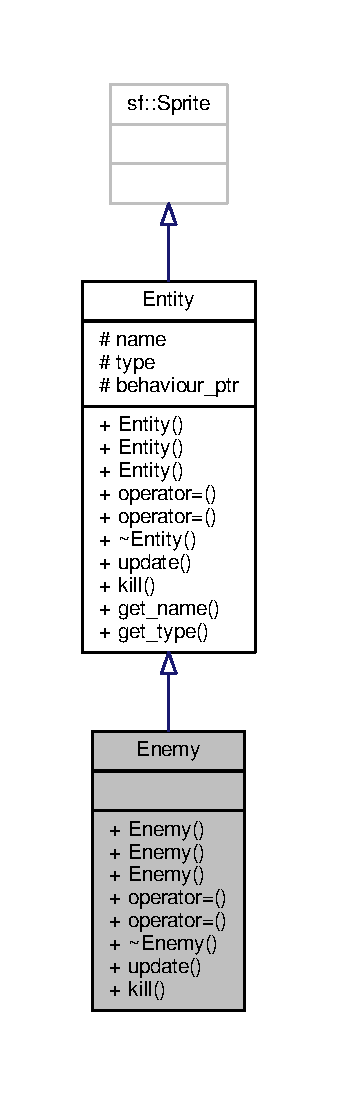
\includegraphics[width=162pt]{classEnemy__inherit__graph}
\end{center}
\end{figure}


Collaboration diagram for Enemy\+:\nopagebreak
\begin{figure}[H]
\begin{center}
\leavevmode
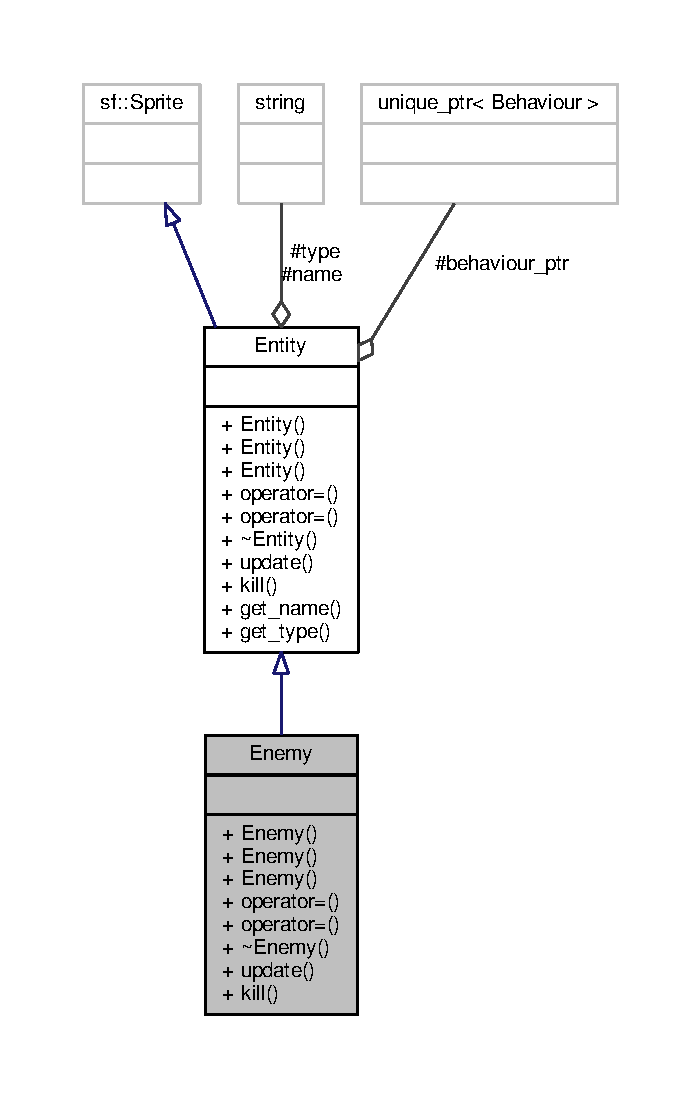
\includegraphics[width=336pt]{classEnemy__coll__graph}
\end{center}
\end{figure}
\subsection*{Public Member Functions}
\begin{DoxyCompactItemize}
\item 
\hyperlink{classEnemy_ae8d63e49373ab8fceaecc652fe489291}{Enemy} (std\+::string, std\+::string, \hyperlink{classBehaviour}{Behaviour} $\ast$, float, float, sf\+::\+Texture const \&, sf\+::\+Int\+Rect)
\item 
\hyperlink{classEnemy_acd0c806f2a8b6383dcfd1f94a59b2c51}{Enemy} (\hyperlink{classEnemy}{Enemy} const \&other)=delete
\begin{DoxyCompactList}\small\item\em Copy konstruktor. \end{DoxyCompactList}\item 
\hyperlink{classEnemy_aab80b7367a9bf32348962adbb80f930b}{Enemy} (\hyperlink{classEnemy}{Enemy} \&\&other)=delete
\begin{DoxyCompactList}\small\item\em Move konstruktor. \end{DoxyCompactList}\item 
\hyperlink{classEnemy}{Enemy} \& \hyperlink{classEnemy_ae1f8ceea084618eb2f18e162c0970fa1}{operator=} (\hyperlink{classEnemy}{Enemy} const \&rhs)\&=delete
\begin{DoxyCompactList}\small\item\em Copy operator. \end{DoxyCompactList}\item 
\hyperlink{classEnemy}{Enemy} \& \hyperlink{classEnemy_adf7f76b8cac299c83f3fed7bcc7fd3b5}{operator=} (\hyperlink{classEnemy}{Enemy} \&\&rhs)=delete
\begin{DoxyCompactList}\small\item\em Move operator. \end{DoxyCompactList}\item 
\hyperlink{classEnemy_aca00fa2f20cea544f52beeb5aa1648f1}{$\sim$\+Enemy} ()=default
\begin{DoxyCompactList}\small\item\em Default destruktor. \end{DoxyCompactList}\item 
void \hyperlink{classEnemy_a257cacd04930ccbfa9545bb5a8dc5be3}{update} (\hyperlink{classWorld}{World} \&, sf\+::\+Time const \&) override
\item 
void \hyperlink{classEnemy_aba8130fd5f8ede411cded7611254ab7a}{kill} (\hyperlink{classWorld}{World} \&) override
\begin{DoxyCompactList}\small\item\em Om det här objektet har dödats så kommer kill att göra det genom att informera \hyperlink{classWorld}{World} om det. \end{DoxyCompactList}\item 
std\+::string \hyperlink{classEntity_a75c7e4aad3df2e053ee5b43169509534}{get\+\_\+name} () const 
\begin{DoxyCompactList}\small\item\em Returnerar namnet på entititen. \end{DoxyCompactList}\item 
std\+::string \hyperlink{classEntity_a0e9ef479c1147e21e5bcb338cb858df2}{get\+\_\+type} () const 
\begin{DoxyCompactList}\small\item\em Returnerar typen på entititen. \end{DoxyCompactList}\end{DoxyCompactItemize}
\subsection*{Protected Attributes}
\begin{DoxyCompactItemize}
\item 
std\+::string \hyperlink{classEntity_a931b21fbdebb1a5963b4bcab5df128f5}{name}
\begin{DoxyCompactList}\small\item\em Namn. \end{DoxyCompactList}\item 
std\+::string \hyperlink{classEntity_a298a9ebf2474bb00874b5ff6a0d637ef}{type}
\begin{DoxyCompactList}\small\item\em Typ. \end{DoxyCompactList}\item 
std\+::unique\+\_\+ptr$<$ \hyperlink{classBehaviour}{Behaviour} $>$ \hyperlink{classEntity_adb6e36848db24e6d48e6d295e19d3972}{behaviour\+\_\+ptr}
\begin{DoxyCompactList}\small\item\em Unik smart-\/pekare till ett objekt av \hyperlink{classBehaviour}{Behaviour} klassen. \end{DoxyCompactList}\end{DoxyCompactItemize}


\subsection{Detailed Description}
\hyperlink{classEnemy}{Enemy} ärver från \hyperlink{classEntity}{Entity} och innehåller all information för en entitet av fiendetyp. 

\hyperlink{classEnemy}{Enemy} ärver från den abstrakta klassen \hyperlink{classEntity}{Entity} och innehåller informationen för den instans av fiender i spelet den representerar. 

\subsection{Constructor \& Destructor Documentation}
\hypertarget{classEnemy_ae8d63e49373ab8fceaecc652fe489291}{\index{Enemy@{Enemy}!Enemy@{Enemy}}
\index{Enemy@{Enemy}!Enemy@{Enemy}}
\subsubsection[{Enemy}]{\setlength{\rightskip}{0pt plus 5cm}Enemy\+::\+Enemy (
\begin{DoxyParamCaption}
\item[{std\+::string}]{n, }
\item[{std\+::string}]{t, }
\item[{{\bf Behaviour} $\ast$}]{b, }
\item[{float}]{x, }
\item[{float}]{y, }
\item[{sf\+::\+Texture const \&}]{texture, }
\item[{sf\+::\+Int\+Rect}]{size}
\end{DoxyParamCaption}
)}}\label{classEnemy_ae8d63e49373ab8fceaecc652fe489291}
\hyperlink{classEnemy}{Enemy} konstruktorn som tar in ett namn, en typ, en beteende pekare, 2 floats för position, en textur och vilken kvadrat som ska visas. \hypertarget{classEnemy_acd0c806f2a8b6383dcfd1f94a59b2c51}{\index{Enemy@{Enemy}!Enemy@{Enemy}}
\index{Enemy@{Enemy}!Enemy@{Enemy}}
\subsubsection[{Enemy}]{\setlength{\rightskip}{0pt plus 5cm}Enemy\+::\+Enemy (
\begin{DoxyParamCaption}
\item[{{\bf Enemy} const \&}]{other}
\end{DoxyParamCaption}
)\hspace{0.3cm}{\ttfamily [delete]}}}\label{classEnemy_acd0c806f2a8b6383dcfd1f94a59b2c51}


Copy konstruktor. 

\hypertarget{classEnemy_aab80b7367a9bf32348962adbb80f930b}{\index{Enemy@{Enemy}!Enemy@{Enemy}}
\index{Enemy@{Enemy}!Enemy@{Enemy}}
\subsubsection[{Enemy}]{\setlength{\rightskip}{0pt plus 5cm}Enemy\+::\+Enemy (
\begin{DoxyParamCaption}
\item[{{\bf Enemy} \&\&}]{other}
\end{DoxyParamCaption}
)\hspace{0.3cm}{\ttfamily [delete]}}}\label{classEnemy_aab80b7367a9bf32348962adbb80f930b}


Move konstruktor. 

\hypertarget{classEnemy_aca00fa2f20cea544f52beeb5aa1648f1}{\index{Enemy@{Enemy}!````~Enemy@{$\sim$\+Enemy}}
\index{````~Enemy@{$\sim$\+Enemy}!Enemy@{Enemy}}
\subsubsection[{$\sim$\+Enemy}]{\setlength{\rightskip}{0pt plus 5cm}Enemy\+::$\sim$\+Enemy (
\begin{DoxyParamCaption}
{}
\end{DoxyParamCaption}
)\hspace{0.3cm}{\ttfamily [default]}}}\label{classEnemy_aca00fa2f20cea544f52beeb5aa1648f1}


Default destruktor. 



\subsection{Member Function Documentation}
\hypertarget{classEntity_a75c7e4aad3df2e053ee5b43169509534}{\index{Enemy@{Enemy}!get\+\_\+name@{get\+\_\+name}}
\index{get\+\_\+name@{get\+\_\+name}!Enemy@{Enemy}}
\subsubsection[{get\+\_\+name}]{\setlength{\rightskip}{0pt plus 5cm}std\+::string Entity\+::get\+\_\+name (
\begin{DoxyParamCaption}
{}
\end{DoxyParamCaption}
) const\hspace{0.3cm}{\ttfamily [inline]}, {\ttfamily [inherited]}}}\label{classEntity_a75c7e4aad3df2e053ee5b43169509534}


Returnerar namnet på entititen. 

\hypertarget{classEntity_a0e9ef479c1147e21e5bcb338cb858df2}{\index{Enemy@{Enemy}!get\+\_\+type@{get\+\_\+type}}
\index{get\+\_\+type@{get\+\_\+type}!Enemy@{Enemy}}
\subsubsection[{get\+\_\+type}]{\setlength{\rightskip}{0pt plus 5cm}std\+::string Entity\+::get\+\_\+type (
\begin{DoxyParamCaption}
{}
\end{DoxyParamCaption}
) const\hspace{0.3cm}{\ttfamily [inline]}, {\ttfamily [inherited]}}}\label{classEntity_a0e9ef479c1147e21e5bcb338cb858df2}


Returnerar typen på entititen. 

\hypertarget{classEnemy_aba8130fd5f8ede411cded7611254ab7a}{\index{Enemy@{Enemy}!kill@{kill}}
\index{kill@{kill}!Enemy@{Enemy}}
\subsubsection[{kill}]{\setlength{\rightskip}{0pt plus 5cm}void Enemy\+::kill (
\begin{DoxyParamCaption}
\item[{{\bf World} \&}]{world}
\end{DoxyParamCaption}
)\hspace{0.3cm}{\ttfamily [override]}, {\ttfamily [virtual]}}}\label{classEnemy_aba8130fd5f8ede411cded7611254ab7a}


Om det här objektet har dödats så kommer kill att göra det genom att informera \hyperlink{classWorld}{World} om det. 



Implements \hyperlink{classEntity_a3d585a30d7f07c50911485825f5496cd}{Entity}.

\hypertarget{classEnemy_ae1f8ceea084618eb2f18e162c0970fa1}{\index{Enemy@{Enemy}!operator=@{operator=}}
\index{operator=@{operator=}!Enemy@{Enemy}}
\subsubsection[{operator=}]{\setlength{\rightskip}{0pt plus 5cm}{\bf Enemy}\& Enemy\+::operator= (
\begin{DoxyParamCaption}
\item[{{\bf Enemy} const \&}]{rhs}
\end{DoxyParamCaption}
)\hspace{0.3cm}{\ttfamily [delete]}}}\label{classEnemy_ae1f8ceea084618eb2f18e162c0970fa1}


Copy operator. 

\hypertarget{classEnemy_adf7f76b8cac299c83f3fed7bcc7fd3b5}{\index{Enemy@{Enemy}!operator=@{operator=}}
\index{operator=@{operator=}!Enemy@{Enemy}}
\subsubsection[{operator=}]{\setlength{\rightskip}{0pt plus 5cm}{\bf Enemy}\& Enemy\+::operator= (
\begin{DoxyParamCaption}
\item[{{\bf Enemy} \&\&}]{rhs}
\end{DoxyParamCaption}
)\hspace{0.3cm}{\ttfamily [delete]}}}\label{classEnemy_adf7f76b8cac299c83f3fed7bcc7fd3b5}


Move operator. 

\hypertarget{classEnemy_a257cacd04930ccbfa9545bb5a8dc5be3}{\index{Enemy@{Enemy}!update@{update}}
\index{update@{update}!Enemy@{Enemy}}
\subsubsection[{update}]{\setlength{\rightskip}{0pt plus 5cm}void Enemy\+::update (
\begin{DoxyParamCaption}
\item[{{\bf World} \&}]{world, }
\item[{sf\+::\+Time const \&}]{t}
\end{DoxyParamCaption}
)\hspace{0.3cm}{\ttfamily [override]}, {\ttfamily [virtual]}}}\label{classEnemy_a257cacd04930ccbfa9545bb5a8dc5be3}
\hyperlink{classEntity_a180102ac6695559b1f8fcf0aee747802}{Entity\+::update()} override Funktion som kallas av world när det här specifika objektet ska uppdatera sig. Det gör sedan detta genom att t.\+ex. flytta på sig och kolla kollisioner. 

Implements \hyperlink{classEntity_a180102ac6695559b1f8fcf0aee747802}{Entity}.



\subsection{Member Data Documentation}
\hypertarget{classEntity_adb6e36848db24e6d48e6d295e19d3972}{\index{Enemy@{Enemy}!behaviour\+\_\+ptr@{behaviour\+\_\+ptr}}
\index{behaviour\+\_\+ptr@{behaviour\+\_\+ptr}!Enemy@{Enemy}}
\subsubsection[{behaviour\+\_\+ptr}]{\setlength{\rightskip}{0pt plus 5cm}std\+::unique\+\_\+ptr$<${\bf Behaviour}$>$ Entity\+::behaviour\+\_\+ptr\hspace{0.3cm}{\ttfamily [protected]}, {\ttfamily [inherited]}}}\label{classEntity_adb6e36848db24e6d48e6d295e19d3972}


Unik smart-\/pekare till ett objekt av \hyperlink{classBehaviour}{Behaviour} klassen. 

\hypertarget{classEntity_a931b21fbdebb1a5963b4bcab5df128f5}{\index{Enemy@{Enemy}!name@{name}}
\index{name@{name}!Enemy@{Enemy}}
\subsubsection[{name}]{\setlength{\rightskip}{0pt plus 5cm}std\+::string Entity\+::name\hspace{0.3cm}{\ttfamily [protected]}, {\ttfamily [inherited]}}}\label{classEntity_a931b21fbdebb1a5963b4bcab5df128f5}


Namn. 

\hypertarget{classEntity_a298a9ebf2474bb00874b5ff6a0d637ef}{\index{Enemy@{Enemy}!type@{type}}
\index{type@{type}!Enemy@{Enemy}}
\subsubsection[{type}]{\setlength{\rightskip}{0pt plus 5cm}std\+::string Entity\+::type\hspace{0.3cm}{\ttfamily [protected]}, {\ttfamily [inherited]}}}\label{classEntity_a298a9ebf2474bb00874b5ff6a0d637ef}


Typ. 



The documentation for this class was generated from the following files\+:\begin{DoxyCompactItemize}
\item 
source/objects/headers/Enemy.\+h\item 
source/objects/imps/Enemy.\+cpp\end{DoxyCompactItemize}

\hypertarget{classEnemy2__Behaviour}{\section{Enemy2\+\_\+\+Behaviour Class Reference}
\label{classEnemy2__Behaviour}\index{Enemy2\+\_\+\+Behaviour@{Enemy2\+\_\+\+Behaviour}}
}


Enemy\+\_\+\+Behaviour2 ärver från \hyperlink{classBehaviour}{Behaviour} och tillhandahåller beteende för fiender.  




{\ttfamily \#include $<$Enemy2\+\_\+\+Behaviour.\+h$>$}



Inheritance diagram for Enemy2\+\_\+\+Behaviour\+:\nopagebreak
\begin{figure}[H]
\begin{center}
\leavevmode
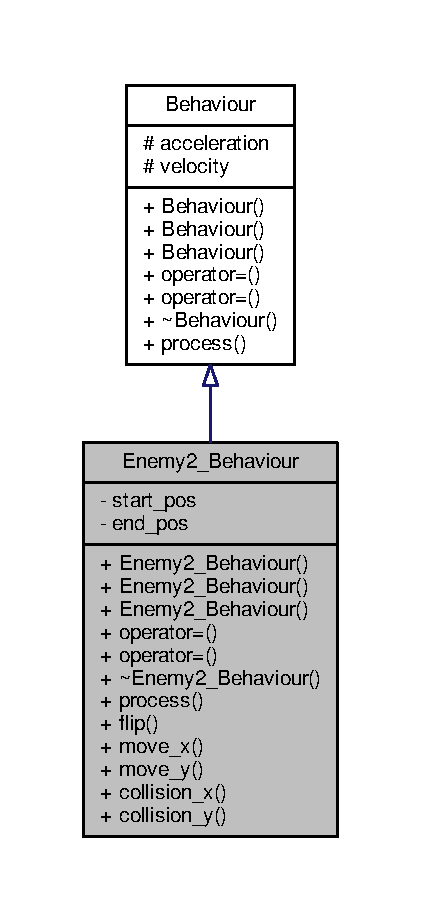
\includegraphics[width=202pt]{classEnemy2__Behaviour__inherit__graph}
\end{center}
\end{figure}


Collaboration diagram for Enemy2\+\_\+\+Behaviour\+:\nopagebreak
\begin{figure}[H]
\begin{center}
\leavevmode
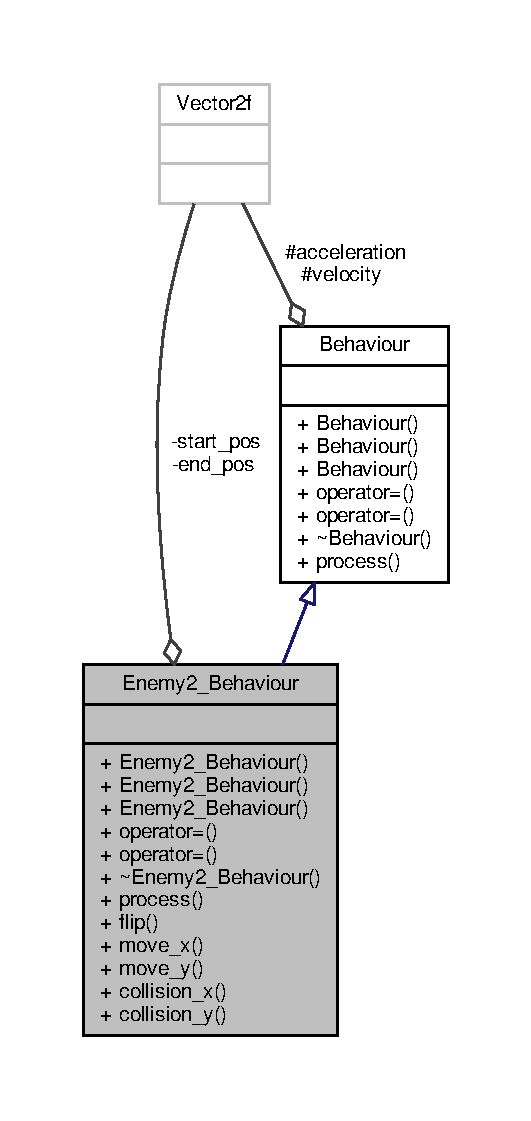
\includegraphics[width=255pt]{classEnemy2__Behaviour__coll__graph}
\end{center}
\end{figure}
\subsection*{Public Member Functions}
\begin{DoxyCompactItemize}
\item 
\hyperlink{classEnemy2__Behaviour_a8a829457bf290b7419955fa8c7808b49}{Enemy2\+\_\+\+Behaviour} (sf\+::\+Vector2f v, float x, float y)
\begin{DoxyCompactList}\small\item\em Vanlig \hyperlink{classBehaviour_a57e050961bc1305993adaeac62658657}{Behaviour\+::\+Behaviour} konstruktor. \end{DoxyCompactList}\item 
\hyperlink{classEnemy2__Behaviour_a12df4777ecea49697eeb5e0185d542dd}{Enemy2\+\_\+\+Behaviour} (\hyperlink{classEnemy2__Behaviour}{Enemy2\+\_\+\+Behaviour} const \&other)=delete
\begin{DoxyCompactList}\small\item\em Copy konstruktor. \end{DoxyCompactList}\item 
\hyperlink{classEnemy2__Behaviour_a17391bee40ff82bd774d0d910048f111}{Enemy2\+\_\+\+Behaviour} (\hyperlink{classEnemy2__Behaviour}{Enemy2\+\_\+\+Behaviour} \&\&other)=delete
\begin{DoxyCompactList}\small\item\em Move konstruktor. \end{DoxyCompactList}\item 
\hyperlink{classEnemy2__Behaviour}{Enemy2\+\_\+\+Behaviour} \& \hyperlink{classEnemy2__Behaviour_aefb93bb199ad534638ae950d6cdd3a24}{operator=} (\hyperlink{classEnemy2__Behaviour}{Enemy2\+\_\+\+Behaviour} const \&rhs)\&=delete
\begin{DoxyCompactList}\small\item\em Copy operator. \end{DoxyCompactList}\item 
\hyperlink{classEnemy2__Behaviour}{Enemy2\+\_\+\+Behaviour} \& \hyperlink{classEnemy2__Behaviour_a640e6d6829df6a9a5ddd14bad50d28a7}{operator=} (\hyperlink{classEnemy2__Behaviour}{Enemy2\+\_\+\+Behaviour} \&\&rhs)=delete
\begin{DoxyCompactList}\small\item\em Move operator. \end{DoxyCompactList}\item 
\hyperlink{classEnemy2__Behaviour_a42f92d6f39b1b14f758da506aaf4bc36}{$\sim$\+Enemy2\+\_\+\+Behaviour} ()=default
\begin{DoxyCompactList}\small\item\em Default destruktor. \end{DoxyCompactList}\item 
void \hyperlink{classEnemy2__Behaviour_a0979bade3f9b3ff9dca3c6b970a5ef63}{process} (\hyperlink{classWorld}{World} \&, \hyperlink{classEntity}{Entity} \&, sf\+::\+Time const \&) override
\begin{DoxyCompactList}\small\item\em Funktionen som låter fienden göra allting. \end{DoxyCompactList}\item 
void \hyperlink{classEnemy2__Behaviour_ad46bf8d3c702e70978b87b36190d2f88}{flip} (\hyperlink{classEntity}{Entity} \&, sf\+::\+Vector2f const \&)
\begin{DoxyCompactList}\small\item\em Funktionen flipar spriten för enemy baserat på vilket håll den rör sig. \end{DoxyCompactList}\item 
void \hyperlink{classEnemy2__Behaviour_a188c7941d10c527271c49ba0bc26baa9}{move\+\_\+x} (\hyperlink{classEntity}{Entity} \&, sf\+::\+Vector2f const \&, sf\+::\+Time)
\begin{DoxyCompactList}\small\item\em Förflyttning i x-\/led. \end{DoxyCompactList}\item 
void \hyperlink{classEnemy2__Behaviour_a535c14bb1fa65c443d35e4e55031418b}{move\+\_\+y} (\hyperlink{classEntity}{Entity} \&, sf\+::\+Vector2f const \&, sf\+::\+Time)
\begin{DoxyCompactList}\small\item\em Förflyttning i y-\/led. \end{DoxyCompactList}\item 
void \hyperlink{classEnemy2__Behaviour_a25d895919b81e15a7e4280d86ded650f}{collision\+\_\+x} (\hyperlink{classWorld}{World} \&, \hyperlink{classEntity}{Entity} \&)
\begin{DoxyCompactList}\small\item\em Kollisionshantering i x-\/led. \end{DoxyCompactList}\item 
void \hyperlink{classEnemy2__Behaviour_a5e89430e0189000bc295db5246c5d380}{collision\+\_\+y} (\hyperlink{classWorld}{World} \&, \hyperlink{classEntity}{Entity} \&)
\begin{DoxyCompactList}\small\item\em Kollisionshantering i y-\/led. \end{DoxyCompactList}\end{DoxyCompactItemize}
\subsection*{Protected Attributes}
\begin{DoxyCompactItemize}
\item 
sf\+::\+Vector2f \hyperlink{classBehaviour_ac17cf81ceee6a44e8a8ec6ee810c9fd3}{acceleration} \{0.\+0f, 0.\+1f\}
\begin{DoxyCompactList}\small\item\em Variabel för gravitation. \end{DoxyCompactList}\item 
sf\+::\+Vector2f \hyperlink{classBehaviour_a1d52096cf20a59890f7705acbaccf88a}{velocity} \{0.\+0f,0.\+0f\}
\begin{DoxyCompactList}\small\item\em Variabel for hastigheten för entiteten. \end{DoxyCompactList}\end{DoxyCompactItemize}
\subsection*{Private Attributes}
\begin{DoxyCompactItemize}
\item 
sf\+::\+Vector2f \hyperlink{classEnemy2__Behaviour_a8adc028fa38366e2e7d204f7da84e34c}{start\+\_\+pos}
\begin{DoxyCompactList}\small\item\em Start positionen. \end{DoxyCompactList}\item 
sf\+::\+Vector2f \hyperlink{classEnemy2__Behaviour_ada807c200f4c5fc5a732d8ada274520a}{end\+\_\+pos}
\begin{DoxyCompactList}\small\item\em Slut positionen. \end{DoxyCompactList}\end{DoxyCompactItemize}


\subsection{Detailed Description}
Enemy\+\_\+\+Behaviour2 ärver från \hyperlink{classBehaviour}{Behaviour} och tillhandahåller beteende för fiender. 

Enemy\+\_\+\+Behaviour2 definerar beteendet för ett \hyperlink{classEnemy}{Enemy} objekt i spelet. \hyperlink{classEnemy}{Enemy} rör sig som \hyperlink{classPlayer__Behaviour}{Player\+\_\+\+Behaviour} men följer spelaren istället för att följa vad användaren anger. Den flipar också \hyperlink{classEnemy}{Enemy} spriten om det behövs och har koll på kollisioner för enemy. \hyperlink{classEnemy}{Enemy} dödar spelaren om de kommer i kontakt med denne.

\hyperlink{classEnemy}{Enemy} nummer 2 rör sig från sin startplats till en ny plats och tillbaka. Detta är det enda den gör. 

\subsection{Constructor \& Destructor Documentation}
\hypertarget{classEnemy2__Behaviour_a8a829457bf290b7419955fa8c7808b49}{\index{Enemy2\+\_\+\+Behaviour@{Enemy2\+\_\+\+Behaviour}!Enemy2\+\_\+\+Behaviour@{Enemy2\+\_\+\+Behaviour}}
\index{Enemy2\+\_\+\+Behaviour@{Enemy2\+\_\+\+Behaviour}!Enemy2\+\_\+\+Behaviour@{Enemy2\+\_\+\+Behaviour}}
\subsubsection[{Enemy2\+\_\+\+Behaviour}]{\setlength{\rightskip}{0pt plus 5cm}Enemy2\+\_\+\+Behaviour\+::\+Enemy2\+\_\+\+Behaviour (
\begin{DoxyParamCaption}
\item[{sf\+::\+Vector2f}]{v, }
\item[{float}]{x, }
\item[{float}]{y}
\end{DoxyParamCaption}
)\hspace{0.3cm}{\ttfamily [inline]}}}\label{classEnemy2__Behaviour_a8a829457bf290b7419955fa8c7808b49}


Vanlig \hyperlink{classBehaviour_a57e050961bc1305993adaeac62658657}{Behaviour\+::\+Behaviour} konstruktor. 

\hypertarget{classEnemy2__Behaviour_a12df4777ecea49697eeb5e0185d542dd}{\index{Enemy2\+\_\+\+Behaviour@{Enemy2\+\_\+\+Behaviour}!Enemy2\+\_\+\+Behaviour@{Enemy2\+\_\+\+Behaviour}}
\index{Enemy2\+\_\+\+Behaviour@{Enemy2\+\_\+\+Behaviour}!Enemy2\+\_\+\+Behaviour@{Enemy2\+\_\+\+Behaviour}}
\subsubsection[{Enemy2\+\_\+\+Behaviour}]{\setlength{\rightskip}{0pt plus 5cm}Enemy2\+\_\+\+Behaviour\+::\+Enemy2\+\_\+\+Behaviour (
\begin{DoxyParamCaption}
\item[{{\bf Enemy2\+\_\+\+Behaviour} const \&}]{other}
\end{DoxyParamCaption}
)\hspace{0.3cm}{\ttfamily [delete]}}}\label{classEnemy2__Behaviour_a12df4777ecea49697eeb5e0185d542dd}


Copy konstruktor. 

\hypertarget{classEnemy2__Behaviour_a17391bee40ff82bd774d0d910048f111}{\index{Enemy2\+\_\+\+Behaviour@{Enemy2\+\_\+\+Behaviour}!Enemy2\+\_\+\+Behaviour@{Enemy2\+\_\+\+Behaviour}}
\index{Enemy2\+\_\+\+Behaviour@{Enemy2\+\_\+\+Behaviour}!Enemy2\+\_\+\+Behaviour@{Enemy2\+\_\+\+Behaviour}}
\subsubsection[{Enemy2\+\_\+\+Behaviour}]{\setlength{\rightskip}{0pt plus 5cm}Enemy2\+\_\+\+Behaviour\+::\+Enemy2\+\_\+\+Behaviour (
\begin{DoxyParamCaption}
\item[{{\bf Enemy2\+\_\+\+Behaviour} \&\&}]{other}
\end{DoxyParamCaption}
)\hspace{0.3cm}{\ttfamily [delete]}}}\label{classEnemy2__Behaviour_a17391bee40ff82bd774d0d910048f111}


Move konstruktor. 

\hypertarget{classEnemy2__Behaviour_a42f92d6f39b1b14f758da506aaf4bc36}{\index{Enemy2\+\_\+\+Behaviour@{Enemy2\+\_\+\+Behaviour}!````~Enemy2\+\_\+\+Behaviour@{$\sim$\+Enemy2\+\_\+\+Behaviour}}
\index{````~Enemy2\+\_\+\+Behaviour@{$\sim$\+Enemy2\+\_\+\+Behaviour}!Enemy2\+\_\+\+Behaviour@{Enemy2\+\_\+\+Behaviour}}
\subsubsection[{$\sim$\+Enemy2\+\_\+\+Behaviour}]{\setlength{\rightskip}{0pt plus 5cm}Enemy2\+\_\+\+Behaviour\+::$\sim$\+Enemy2\+\_\+\+Behaviour (
\begin{DoxyParamCaption}
{}
\end{DoxyParamCaption}
)\hspace{0.3cm}{\ttfamily [default]}}}\label{classEnemy2__Behaviour_a42f92d6f39b1b14f758da506aaf4bc36}


Default destruktor. 



\subsection{Member Function Documentation}
\hypertarget{classEnemy2__Behaviour_a25d895919b81e15a7e4280d86ded650f}{\index{Enemy2\+\_\+\+Behaviour@{Enemy2\+\_\+\+Behaviour}!collision\+\_\+x@{collision\+\_\+x}}
\index{collision\+\_\+x@{collision\+\_\+x}!Enemy2\+\_\+\+Behaviour@{Enemy2\+\_\+\+Behaviour}}
\subsubsection[{collision\+\_\+x}]{\setlength{\rightskip}{0pt plus 5cm}void Enemy2\+\_\+\+Behaviour\+::collision\+\_\+x (
\begin{DoxyParamCaption}
\item[{{\bf World} \&}]{world, }
\item[{{\bf Entity} \&}]{owner}
\end{DoxyParamCaption}
)}}\label{classEnemy2__Behaviour_a25d895919b81e15a7e4280d86ded650f}


Kollisionshantering i x-\/led. 

\hypertarget{classEnemy2__Behaviour_a5e89430e0189000bc295db5246c5d380}{\index{Enemy2\+\_\+\+Behaviour@{Enemy2\+\_\+\+Behaviour}!collision\+\_\+y@{collision\+\_\+y}}
\index{collision\+\_\+y@{collision\+\_\+y}!Enemy2\+\_\+\+Behaviour@{Enemy2\+\_\+\+Behaviour}}
\subsubsection[{collision\+\_\+y}]{\setlength{\rightskip}{0pt plus 5cm}void Enemy2\+\_\+\+Behaviour\+::collision\+\_\+y (
\begin{DoxyParamCaption}
\item[{{\bf World} \&}]{world, }
\item[{{\bf Entity} \&}]{owner}
\end{DoxyParamCaption}
)}}\label{classEnemy2__Behaviour_a5e89430e0189000bc295db5246c5d380}


Kollisionshantering i y-\/led. 

\hypertarget{classEnemy2__Behaviour_ad46bf8d3c702e70978b87b36190d2f88}{\index{Enemy2\+\_\+\+Behaviour@{Enemy2\+\_\+\+Behaviour}!flip@{flip}}
\index{flip@{flip}!Enemy2\+\_\+\+Behaviour@{Enemy2\+\_\+\+Behaviour}}
\subsubsection[{flip}]{\setlength{\rightskip}{0pt plus 5cm}void Enemy2\+\_\+\+Behaviour\+::flip (
\begin{DoxyParamCaption}
\item[{{\bf Entity} \&}]{owner, }
\item[{sf\+::\+Vector2f const \&}]{dir}
\end{DoxyParamCaption}
)}}\label{classEnemy2__Behaviour_ad46bf8d3c702e70978b87b36190d2f88}


Funktionen flipar spriten för enemy baserat på vilket håll den rör sig. 

\hypertarget{classEnemy2__Behaviour_a188c7941d10c527271c49ba0bc26baa9}{\index{Enemy2\+\_\+\+Behaviour@{Enemy2\+\_\+\+Behaviour}!move\+\_\+x@{move\+\_\+x}}
\index{move\+\_\+x@{move\+\_\+x}!Enemy2\+\_\+\+Behaviour@{Enemy2\+\_\+\+Behaviour}}
\subsubsection[{move\+\_\+x}]{\setlength{\rightskip}{0pt plus 5cm}void Enemy2\+\_\+\+Behaviour\+::move\+\_\+x (
\begin{DoxyParamCaption}
\item[{{\bf Entity} \&}]{owner, }
\item[{sf\+::\+Vector2f const \&}]{dir, }
\item[{sf\+::\+Time}]{t}
\end{DoxyParamCaption}
)}}\label{classEnemy2__Behaviour_a188c7941d10c527271c49ba0bc26baa9}


Förflyttning i x-\/led. 

\hypertarget{classEnemy2__Behaviour_a535c14bb1fa65c443d35e4e55031418b}{\index{Enemy2\+\_\+\+Behaviour@{Enemy2\+\_\+\+Behaviour}!move\+\_\+y@{move\+\_\+y}}
\index{move\+\_\+y@{move\+\_\+y}!Enemy2\+\_\+\+Behaviour@{Enemy2\+\_\+\+Behaviour}}
\subsubsection[{move\+\_\+y}]{\setlength{\rightskip}{0pt plus 5cm}void Enemy2\+\_\+\+Behaviour\+::move\+\_\+y (
\begin{DoxyParamCaption}
\item[{{\bf Entity} \&}]{owner, }
\item[{sf\+::\+Vector2f const \&}]{dir, }
\item[{sf\+::\+Time}]{t}
\end{DoxyParamCaption}
)}}\label{classEnemy2__Behaviour_a535c14bb1fa65c443d35e4e55031418b}


Förflyttning i y-\/led. 

\hypertarget{classEnemy2__Behaviour_aefb93bb199ad534638ae950d6cdd3a24}{\index{Enemy2\+\_\+\+Behaviour@{Enemy2\+\_\+\+Behaviour}!operator=@{operator=}}
\index{operator=@{operator=}!Enemy2\+\_\+\+Behaviour@{Enemy2\+\_\+\+Behaviour}}
\subsubsection[{operator=}]{\setlength{\rightskip}{0pt plus 5cm}{\bf Enemy2\+\_\+\+Behaviour}\& Enemy2\+\_\+\+Behaviour\+::operator= (
\begin{DoxyParamCaption}
\item[{{\bf Enemy2\+\_\+\+Behaviour} const \&}]{rhs}
\end{DoxyParamCaption}
)\hspace{0.3cm}{\ttfamily [delete]}}}\label{classEnemy2__Behaviour_aefb93bb199ad534638ae950d6cdd3a24}


Copy operator. 

\hypertarget{classEnemy2__Behaviour_a640e6d6829df6a9a5ddd14bad50d28a7}{\index{Enemy2\+\_\+\+Behaviour@{Enemy2\+\_\+\+Behaviour}!operator=@{operator=}}
\index{operator=@{operator=}!Enemy2\+\_\+\+Behaviour@{Enemy2\+\_\+\+Behaviour}}
\subsubsection[{operator=}]{\setlength{\rightskip}{0pt plus 5cm}{\bf Enemy2\+\_\+\+Behaviour}\& Enemy2\+\_\+\+Behaviour\+::operator= (
\begin{DoxyParamCaption}
\item[{{\bf Enemy2\+\_\+\+Behaviour} \&\&}]{rhs}
\end{DoxyParamCaption}
)\hspace{0.3cm}{\ttfamily [delete]}}}\label{classEnemy2__Behaviour_a640e6d6829df6a9a5ddd14bad50d28a7}


Move operator. 

\hypertarget{classEnemy2__Behaviour_a0979bade3f9b3ff9dca3c6b970a5ef63}{\index{Enemy2\+\_\+\+Behaviour@{Enemy2\+\_\+\+Behaviour}!process@{process}}
\index{process@{process}!Enemy2\+\_\+\+Behaviour@{Enemy2\+\_\+\+Behaviour}}
\subsubsection[{process}]{\setlength{\rightskip}{0pt plus 5cm}void Enemy2\+\_\+\+Behaviour\+::process (
\begin{DoxyParamCaption}
\item[{{\bf World} \&}]{world, }
\item[{{\bf Entity} \&}]{owner, }
\item[{sf\+::\+Time const \&}]{t}
\end{DoxyParamCaption}
)\hspace{0.3cm}{\ttfamily [override]}, {\ttfamily [virtual]}}}\label{classEnemy2__Behaviour_a0979bade3f9b3ff9dca3c6b970a5ef63}


Funktionen som låter fienden göra allting. 



Implements \hyperlink{classBehaviour_aaa6b4ee24dc3cc546fa4dbb7ba4d20da}{Behaviour}.



\subsection{Member Data Documentation}
\hypertarget{classBehaviour_ac17cf81ceee6a44e8a8ec6ee810c9fd3}{\index{Enemy2\+\_\+\+Behaviour@{Enemy2\+\_\+\+Behaviour}!acceleration@{acceleration}}
\index{acceleration@{acceleration}!Enemy2\+\_\+\+Behaviour@{Enemy2\+\_\+\+Behaviour}}
\subsubsection[{acceleration}]{\setlength{\rightskip}{0pt plus 5cm}sf\+::\+Vector2f Behaviour\+::acceleration \{0.\+0f, 0.\+1f\}\hspace{0.3cm}{\ttfamily [protected]}, {\ttfamily [inherited]}}}\label{classBehaviour_ac17cf81ceee6a44e8a8ec6ee810c9fd3}


Variabel för gravitation. 

\hypertarget{classEnemy2__Behaviour_ada807c200f4c5fc5a732d8ada274520a}{\index{Enemy2\+\_\+\+Behaviour@{Enemy2\+\_\+\+Behaviour}!end\+\_\+pos@{end\+\_\+pos}}
\index{end\+\_\+pos@{end\+\_\+pos}!Enemy2\+\_\+\+Behaviour@{Enemy2\+\_\+\+Behaviour}}
\subsubsection[{end\+\_\+pos}]{\setlength{\rightskip}{0pt plus 5cm}sf\+::\+Vector2f Enemy2\+\_\+\+Behaviour\+::end\+\_\+pos\hspace{0.3cm}{\ttfamily [private]}}}\label{classEnemy2__Behaviour_ada807c200f4c5fc5a732d8ada274520a}


Slut positionen. 

\hypertarget{classEnemy2__Behaviour_a8adc028fa38366e2e7d204f7da84e34c}{\index{Enemy2\+\_\+\+Behaviour@{Enemy2\+\_\+\+Behaviour}!start\+\_\+pos@{start\+\_\+pos}}
\index{start\+\_\+pos@{start\+\_\+pos}!Enemy2\+\_\+\+Behaviour@{Enemy2\+\_\+\+Behaviour}}
\subsubsection[{start\+\_\+pos}]{\setlength{\rightskip}{0pt plus 5cm}sf\+::\+Vector2f Enemy2\+\_\+\+Behaviour\+::start\+\_\+pos\hspace{0.3cm}{\ttfamily [private]}}}\label{classEnemy2__Behaviour_a8adc028fa38366e2e7d204f7da84e34c}


Start positionen. 

\hypertarget{classBehaviour_a1d52096cf20a59890f7705acbaccf88a}{\index{Enemy2\+\_\+\+Behaviour@{Enemy2\+\_\+\+Behaviour}!velocity@{velocity}}
\index{velocity@{velocity}!Enemy2\+\_\+\+Behaviour@{Enemy2\+\_\+\+Behaviour}}
\subsubsection[{velocity}]{\setlength{\rightskip}{0pt plus 5cm}sf\+::\+Vector2f Behaviour\+::velocity \{0.\+0f,0.\+0f\}\hspace{0.3cm}{\ttfamily [protected]}, {\ttfamily [inherited]}}}\label{classBehaviour_a1d52096cf20a59890f7705acbaccf88a}


Variabel for hastigheten för entiteten. 



The documentation for this class was generated from the following files\+:\begin{DoxyCompactItemize}
\item 
source/objects/headers/Enemy2\+\_\+\+Behaviour.\+h\item 
source/objects/imps/Enemy2\+\_\+\+Behaviour.\+cpp\end{DoxyCompactItemize}

\hypertarget{classEnemy__Behaviour}{\section{Enemy\+\_\+\+Behaviour Class Reference}
\label{classEnemy__Behaviour}\index{Enemy\+\_\+\+Behaviour@{Enemy\+\_\+\+Behaviour}}
}


\hyperlink{classEnemy__Behaviour}{Enemy\+\_\+\+Behaviour} ärver från \hyperlink{classBehaviour}{Behaviour} och tillhandahåller beteende för fiender.  




{\ttfamily \#include $<$Enemy\+\_\+\+Behaviour.\+h$>$}



Inheritance diagram for Enemy\+\_\+\+Behaviour\+:\nopagebreak
\begin{figure}[H]
\begin{center}
\leavevmode
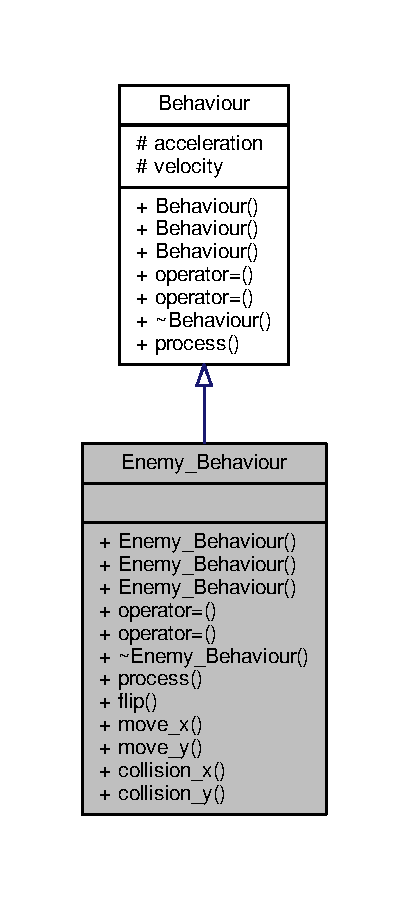
\includegraphics[width=196pt]{classEnemy__Behaviour__inherit__graph}
\end{center}
\end{figure}


Collaboration diagram for Enemy\+\_\+\+Behaviour\+:\nopagebreak
\begin{figure}[H]
\begin{center}
\leavevmode
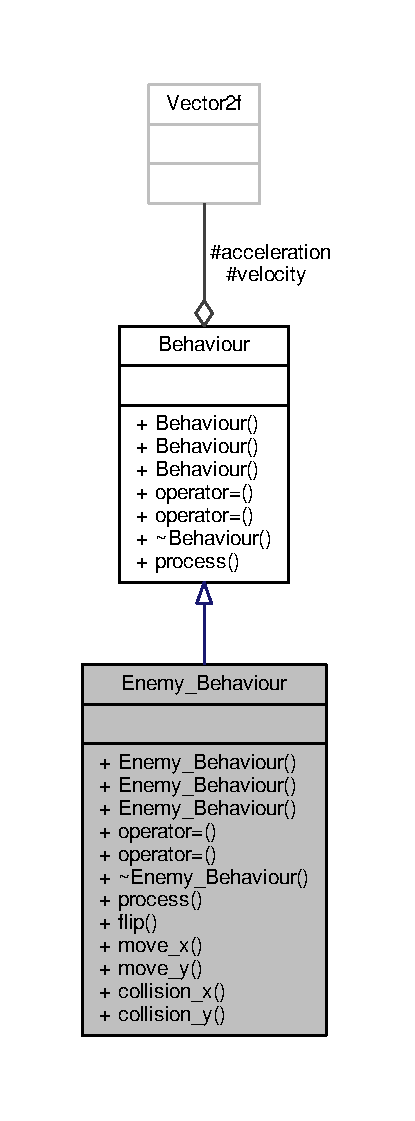
\includegraphics[width=199pt]{classEnemy__Behaviour__coll__graph}
\end{center}
\end{figure}
\subsection*{Public Member Functions}
\begin{DoxyCompactItemize}
\item 
\hyperlink{classEnemy__Behaviour_a7f9664c16fb8882fb8fde685a965252e}{Enemy\+\_\+\+Behaviour} ()
\begin{DoxyCompactList}\small\item\em Vanlig \hyperlink{classBehaviour_a57e050961bc1305993adaeac62658657}{Behaviour\+::\+Behaviour} konstruktor. \end{DoxyCompactList}\item 
\hyperlink{classEnemy__Behaviour_acdcb3d585dd17edc510f0c24f956b798}{Enemy\+\_\+\+Behaviour} (\hyperlink{classEnemy__Behaviour}{Enemy\+\_\+\+Behaviour} const \&other)=delete
\begin{DoxyCompactList}\small\item\em Copy konstruktor. \end{DoxyCompactList}\item 
\hyperlink{classEnemy__Behaviour_ac46de3386a52bc87075f46f0c8b5e60d}{Enemy\+\_\+\+Behaviour} (\hyperlink{classEnemy__Behaviour}{Enemy\+\_\+\+Behaviour} \&\&other)=delete
\begin{DoxyCompactList}\small\item\em Move konstruktor. \end{DoxyCompactList}\item 
\hyperlink{classEnemy__Behaviour}{Enemy\+\_\+\+Behaviour} \& \hyperlink{classEnemy__Behaviour_a11392864d130739b2926f63c21d6fa77}{operator=} (\hyperlink{classEnemy__Behaviour}{Enemy\+\_\+\+Behaviour} const \&rhs)\&=delete
\begin{DoxyCompactList}\small\item\em Copy operator. \end{DoxyCompactList}\item 
\hyperlink{classEnemy__Behaviour}{Enemy\+\_\+\+Behaviour} \& \hyperlink{classEnemy__Behaviour_aae622d7ae52b4c03bdceec9f2081a34f}{operator=} (\hyperlink{classEnemy__Behaviour}{Enemy\+\_\+\+Behaviour} \&\&rhs)=delete
\begin{DoxyCompactList}\small\item\em Move operator. \end{DoxyCompactList}\item 
\hyperlink{classEnemy__Behaviour_ab04de6117d4cbb5fe310b022e9f2de96}{$\sim$\+Enemy\+\_\+\+Behaviour} ()=default
\begin{DoxyCompactList}\small\item\em Default destruktor. \end{DoxyCompactList}\item 
void \hyperlink{classEnemy__Behaviour_a19097e215910b3fd8cf9e002a6f7f642}{process} (\hyperlink{classWorld}{World} \&, \hyperlink{classEntity}{Entity} \&, sf\+::\+Time const \&) override
\begin{DoxyCompactList}\small\item\em Funktionen som låter fienden göra allting. \end{DoxyCompactList}\item 
void \hyperlink{classEnemy__Behaviour_a539ca31dbfab9b02933d6c8ad53b6899}{flip} (\hyperlink{classEntity}{Entity} \&, sf\+::\+Vector2f const \&)
\begin{DoxyCompactList}\small\item\em Funktionen flipar spriten för enemy baserat på vilket håll den rör sig. \end{DoxyCompactList}\item 
void \hyperlink{classEnemy__Behaviour_a4c16df5a815e62dcc41450a997d45cbb}{move\+\_\+x} (\hyperlink{classEntity}{Entity} \&, sf\+::\+Vector2f const \&, sf\+::\+Time)
\begin{DoxyCompactList}\small\item\em Förflyttning i x-\/led. \end{DoxyCompactList}\item 
void \hyperlink{classEnemy__Behaviour_a2793ee5dfc35eff84ba7894619dec0ef}{move\+\_\+y} (\hyperlink{classEntity}{Entity} \&, sf\+::\+Vector2f const \&, sf\+::\+Time)
\begin{DoxyCompactList}\small\item\em Förflyttning i y-\/led. \end{DoxyCompactList}\item 
void \hyperlink{classEnemy__Behaviour_a33b00ea5e572f8084f48891c0f951048}{collision\+\_\+x} (\hyperlink{classWorld}{World} \&, \hyperlink{classEntity}{Entity} \&)
\begin{DoxyCompactList}\small\item\em Kollisionshantering i x-\/led. \end{DoxyCompactList}\item 
void \hyperlink{classEnemy__Behaviour_a67c1e90d31e938cd6a064064a5f97fbc}{collision\+\_\+y} (\hyperlink{classWorld}{World} \&, \hyperlink{classEntity}{Entity} \&)
\begin{DoxyCompactList}\small\item\em Kollisionshantering i y-\/led. \end{DoxyCompactList}\end{DoxyCompactItemize}
\subsection*{Protected Attributes}
\begin{DoxyCompactItemize}
\item 
sf\+::\+Vector2f \hyperlink{classBehaviour_ac17cf81ceee6a44e8a8ec6ee810c9fd3}{acceleration} \{0.\+0f, 0.\+1f\}
\begin{DoxyCompactList}\small\item\em Variabel för gravitation. \end{DoxyCompactList}\item 
sf\+::\+Vector2f \hyperlink{classBehaviour_a1d52096cf20a59890f7705acbaccf88a}{velocity} \{0.\+0f,0.\+0f\}
\begin{DoxyCompactList}\small\item\em Variabel for hastigheten för entiteten. \end{DoxyCompactList}\end{DoxyCompactItemize}


\subsection{Detailed Description}
\hyperlink{classEnemy__Behaviour}{Enemy\+\_\+\+Behaviour} ärver från \hyperlink{classBehaviour}{Behaviour} och tillhandahåller beteende för fiender. 

\hyperlink{classEnemy__Behaviour}{Enemy\+\_\+\+Behaviour} definerar beteendet för ett \hyperlink{classEnemy}{Enemy} objekt i spelet. \hyperlink{classEnemy}{Enemy} rör sig som \hyperlink{classPlayer__Behaviour}{Player\+\_\+\+Behaviour} men följer spelaren istället för att följa vad användaren anger. Den flipar också \hyperlink{classEnemy}{Enemy} spriten om det behövs och har koll på kollisioner för enemy. \hyperlink{classEnemy}{Enemy} dödar spelaren om de kommer i kontakt med denne.

\hyperlink{classEnemy}{Enemy} nummer 1 följer spelarens movement och försöker anfalla den. 

\subsection{Constructor \& Destructor Documentation}
\hypertarget{classEnemy__Behaviour_a7f9664c16fb8882fb8fde685a965252e}{\index{Enemy\+\_\+\+Behaviour@{Enemy\+\_\+\+Behaviour}!Enemy\+\_\+\+Behaviour@{Enemy\+\_\+\+Behaviour}}
\index{Enemy\+\_\+\+Behaviour@{Enemy\+\_\+\+Behaviour}!Enemy\+\_\+\+Behaviour@{Enemy\+\_\+\+Behaviour}}
\subsubsection[{Enemy\+\_\+\+Behaviour}]{\setlength{\rightskip}{0pt plus 5cm}Enemy\+\_\+\+Behaviour\+::\+Enemy\+\_\+\+Behaviour (
\begin{DoxyParamCaption}
{}
\end{DoxyParamCaption}
)\hspace{0.3cm}{\ttfamily [inline]}}}\label{classEnemy__Behaviour_a7f9664c16fb8882fb8fde685a965252e}


Vanlig \hyperlink{classBehaviour_a57e050961bc1305993adaeac62658657}{Behaviour\+::\+Behaviour} konstruktor. 

\hypertarget{classEnemy__Behaviour_acdcb3d585dd17edc510f0c24f956b798}{\index{Enemy\+\_\+\+Behaviour@{Enemy\+\_\+\+Behaviour}!Enemy\+\_\+\+Behaviour@{Enemy\+\_\+\+Behaviour}}
\index{Enemy\+\_\+\+Behaviour@{Enemy\+\_\+\+Behaviour}!Enemy\+\_\+\+Behaviour@{Enemy\+\_\+\+Behaviour}}
\subsubsection[{Enemy\+\_\+\+Behaviour}]{\setlength{\rightskip}{0pt plus 5cm}Enemy\+\_\+\+Behaviour\+::\+Enemy\+\_\+\+Behaviour (
\begin{DoxyParamCaption}
\item[{{\bf Enemy\+\_\+\+Behaviour} const \&}]{other}
\end{DoxyParamCaption}
)\hspace{0.3cm}{\ttfamily [delete]}}}\label{classEnemy__Behaviour_acdcb3d585dd17edc510f0c24f956b798}


Copy konstruktor. 

\hypertarget{classEnemy__Behaviour_ac46de3386a52bc87075f46f0c8b5e60d}{\index{Enemy\+\_\+\+Behaviour@{Enemy\+\_\+\+Behaviour}!Enemy\+\_\+\+Behaviour@{Enemy\+\_\+\+Behaviour}}
\index{Enemy\+\_\+\+Behaviour@{Enemy\+\_\+\+Behaviour}!Enemy\+\_\+\+Behaviour@{Enemy\+\_\+\+Behaviour}}
\subsubsection[{Enemy\+\_\+\+Behaviour}]{\setlength{\rightskip}{0pt plus 5cm}Enemy\+\_\+\+Behaviour\+::\+Enemy\+\_\+\+Behaviour (
\begin{DoxyParamCaption}
\item[{{\bf Enemy\+\_\+\+Behaviour} \&\&}]{other}
\end{DoxyParamCaption}
)\hspace{0.3cm}{\ttfamily [delete]}}}\label{classEnemy__Behaviour_ac46de3386a52bc87075f46f0c8b5e60d}


Move konstruktor. 

\hypertarget{classEnemy__Behaviour_ab04de6117d4cbb5fe310b022e9f2de96}{\index{Enemy\+\_\+\+Behaviour@{Enemy\+\_\+\+Behaviour}!````~Enemy\+\_\+\+Behaviour@{$\sim$\+Enemy\+\_\+\+Behaviour}}
\index{````~Enemy\+\_\+\+Behaviour@{$\sim$\+Enemy\+\_\+\+Behaviour}!Enemy\+\_\+\+Behaviour@{Enemy\+\_\+\+Behaviour}}
\subsubsection[{$\sim$\+Enemy\+\_\+\+Behaviour}]{\setlength{\rightskip}{0pt plus 5cm}Enemy\+\_\+\+Behaviour\+::$\sim$\+Enemy\+\_\+\+Behaviour (
\begin{DoxyParamCaption}
{}
\end{DoxyParamCaption}
)\hspace{0.3cm}{\ttfamily [default]}}}\label{classEnemy__Behaviour_ab04de6117d4cbb5fe310b022e9f2de96}


Default destruktor. 



\subsection{Member Function Documentation}
\hypertarget{classEnemy__Behaviour_a33b00ea5e572f8084f48891c0f951048}{\index{Enemy\+\_\+\+Behaviour@{Enemy\+\_\+\+Behaviour}!collision\+\_\+x@{collision\+\_\+x}}
\index{collision\+\_\+x@{collision\+\_\+x}!Enemy\+\_\+\+Behaviour@{Enemy\+\_\+\+Behaviour}}
\subsubsection[{collision\+\_\+x}]{\setlength{\rightskip}{0pt plus 5cm}void Enemy\+\_\+\+Behaviour\+::collision\+\_\+x (
\begin{DoxyParamCaption}
\item[{{\bf World} \&}]{world, }
\item[{{\bf Entity} \&}]{owner}
\end{DoxyParamCaption}
)}}\label{classEnemy__Behaviour_a33b00ea5e572f8084f48891c0f951048}


Kollisionshantering i x-\/led. 

\hypertarget{classEnemy__Behaviour_a67c1e90d31e938cd6a064064a5f97fbc}{\index{Enemy\+\_\+\+Behaviour@{Enemy\+\_\+\+Behaviour}!collision\+\_\+y@{collision\+\_\+y}}
\index{collision\+\_\+y@{collision\+\_\+y}!Enemy\+\_\+\+Behaviour@{Enemy\+\_\+\+Behaviour}}
\subsubsection[{collision\+\_\+y}]{\setlength{\rightskip}{0pt plus 5cm}void Enemy\+\_\+\+Behaviour\+::collision\+\_\+y (
\begin{DoxyParamCaption}
\item[{{\bf World} \&}]{world, }
\item[{{\bf Entity} \&}]{owner}
\end{DoxyParamCaption}
)}}\label{classEnemy__Behaviour_a67c1e90d31e938cd6a064064a5f97fbc}


Kollisionshantering i y-\/led. 

\hypertarget{classEnemy__Behaviour_a539ca31dbfab9b02933d6c8ad53b6899}{\index{Enemy\+\_\+\+Behaviour@{Enemy\+\_\+\+Behaviour}!flip@{flip}}
\index{flip@{flip}!Enemy\+\_\+\+Behaviour@{Enemy\+\_\+\+Behaviour}}
\subsubsection[{flip}]{\setlength{\rightskip}{0pt plus 5cm}void Enemy\+\_\+\+Behaviour\+::flip (
\begin{DoxyParamCaption}
\item[{{\bf Entity} \&}]{owner, }
\item[{sf\+::\+Vector2f const \&}]{dir}
\end{DoxyParamCaption}
)}}\label{classEnemy__Behaviour_a539ca31dbfab9b02933d6c8ad53b6899}


Funktionen flipar spriten för enemy baserat på vilket håll den rör sig. 

\hypertarget{classEnemy__Behaviour_a4c16df5a815e62dcc41450a997d45cbb}{\index{Enemy\+\_\+\+Behaviour@{Enemy\+\_\+\+Behaviour}!move\+\_\+x@{move\+\_\+x}}
\index{move\+\_\+x@{move\+\_\+x}!Enemy\+\_\+\+Behaviour@{Enemy\+\_\+\+Behaviour}}
\subsubsection[{move\+\_\+x}]{\setlength{\rightskip}{0pt plus 5cm}void Enemy\+\_\+\+Behaviour\+::move\+\_\+x (
\begin{DoxyParamCaption}
\item[{{\bf Entity} \&}]{owner, }
\item[{sf\+::\+Vector2f const \&}]{dir, }
\item[{sf\+::\+Time}]{t}
\end{DoxyParamCaption}
)}}\label{classEnemy__Behaviour_a4c16df5a815e62dcc41450a997d45cbb}


Förflyttning i x-\/led. 

\hypertarget{classEnemy__Behaviour_a2793ee5dfc35eff84ba7894619dec0ef}{\index{Enemy\+\_\+\+Behaviour@{Enemy\+\_\+\+Behaviour}!move\+\_\+y@{move\+\_\+y}}
\index{move\+\_\+y@{move\+\_\+y}!Enemy\+\_\+\+Behaviour@{Enemy\+\_\+\+Behaviour}}
\subsubsection[{move\+\_\+y}]{\setlength{\rightskip}{0pt plus 5cm}void Enemy\+\_\+\+Behaviour\+::move\+\_\+y (
\begin{DoxyParamCaption}
\item[{{\bf Entity} \&}]{owner, }
\item[{sf\+::\+Vector2f const \&}]{dir, }
\item[{sf\+::\+Time}]{t}
\end{DoxyParamCaption}
)}}\label{classEnemy__Behaviour_a2793ee5dfc35eff84ba7894619dec0ef}


Förflyttning i y-\/led. 

\hypertarget{classEnemy__Behaviour_a11392864d130739b2926f63c21d6fa77}{\index{Enemy\+\_\+\+Behaviour@{Enemy\+\_\+\+Behaviour}!operator=@{operator=}}
\index{operator=@{operator=}!Enemy\+\_\+\+Behaviour@{Enemy\+\_\+\+Behaviour}}
\subsubsection[{operator=}]{\setlength{\rightskip}{0pt plus 5cm}{\bf Enemy\+\_\+\+Behaviour}\& Enemy\+\_\+\+Behaviour\+::operator= (
\begin{DoxyParamCaption}
\item[{{\bf Enemy\+\_\+\+Behaviour} const \&}]{rhs}
\end{DoxyParamCaption}
)\hspace{0.3cm}{\ttfamily [delete]}}}\label{classEnemy__Behaviour_a11392864d130739b2926f63c21d6fa77}


Copy operator. 

\hypertarget{classEnemy__Behaviour_aae622d7ae52b4c03bdceec9f2081a34f}{\index{Enemy\+\_\+\+Behaviour@{Enemy\+\_\+\+Behaviour}!operator=@{operator=}}
\index{operator=@{operator=}!Enemy\+\_\+\+Behaviour@{Enemy\+\_\+\+Behaviour}}
\subsubsection[{operator=}]{\setlength{\rightskip}{0pt plus 5cm}{\bf Enemy\+\_\+\+Behaviour}\& Enemy\+\_\+\+Behaviour\+::operator= (
\begin{DoxyParamCaption}
\item[{{\bf Enemy\+\_\+\+Behaviour} \&\&}]{rhs}
\end{DoxyParamCaption}
)\hspace{0.3cm}{\ttfamily [delete]}}}\label{classEnemy__Behaviour_aae622d7ae52b4c03bdceec9f2081a34f}


Move operator. 

\hypertarget{classEnemy__Behaviour_a19097e215910b3fd8cf9e002a6f7f642}{\index{Enemy\+\_\+\+Behaviour@{Enemy\+\_\+\+Behaviour}!process@{process}}
\index{process@{process}!Enemy\+\_\+\+Behaviour@{Enemy\+\_\+\+Behaviour}}
\subsubsection[{process}]{\setlength{\rightskip}{0pt plus 5cm}void Enemy\+\_\+\+Behaviour\+::process (
\begin{DoxyParamCaption}
\item[{{\bf World} \&}]{world, }
\item[{{\bf Entity} \&}]{owner, }
\item[{sf\+::\+Time const \&}]{t}
\end{DoxyParamCaption}
)\hspace{0.3cm}{\ttfamily [override]}, {\ttfamily [virtual]}}}\label{classEnemy__Behaviour_a19097e215910b3fd8cf9e002a6f7f642}


Funktionen som låter fienden göra allting. 



Implements \hyperlink{classBehaviour_aaa6b4ee24dc3cc546fa4dbb7ba4d20da}{Behaviour}.



\subsection{Member Data Documentation}
\hypertarget{classBehaviour_ac17cf81ceee6a44e8a8ec6ee810c9fd3}{\index{Enemy\+\_\+\+Behaviour@{Enemy\+\_\+\+Behaviour}!acceleration@{acceleration}}
\index{acceleration@{acceleration}!Enemy\+\_\+\+Behaviour@{Enemy\+\_\+\+Behaviour}}
\subsubsection[{acceleration}]{\setlength{\rightskip}{0pt plus 5cm}sf\+::\+Vector2f Behaviour\+::acceleration \{0.\+0f, 0.\+1f\}\hspace{0.3cm}{\ttfamily [protected]}, {\ttfamily [inherited]}}}\label{classBehaviour_ac17cf81ceee6a44e8a8ec6ee810c9fd3}


Variabel för gravitation. 

\hypertarget{classBehaviour_a1d52096cf20a59890f7705acbaccf88a}{\index{Enemy\+\_\+\+Behaviour@{Enemy\+\_\+\+Behaviour}!velocity@{velocity}}
\index{velocity@{velocity}!Enemy\+\_\+\+Behaviour@{Enemy\+\_\+\+Behaviour}}
\subsubsection[{velocity}]{\setlength{\rightskip}{0pt plus 5cm}sf\+::\+Vector2f Behaviour\+::velocity \{0.\+0f,0.\+0f\}\hspace{0.3cm}{\ttfamily [protected]}, {\ttfamily [inherited]}}}\label{classBehaviour_a1d52096cf20a59890f7705acbaccf88a}


Variabel for hastigheten för entiteten. 



The documentation for this class was generated from the following files\+:\begin{DoxyCompactItemize}
\item 
source/objects/headers/Enemy\+\_\+\+Behaviour.\+h\item 
source/objects/imps/Enemy\+\_\+\+Behaviour.\+cpp\end{DoxyCompactItemize}

\hypertarget{classEntity}{\section{Entity Class Reference}
\label{classEntity}\index{Entity@{Entity}}
}


\hyperlink{classEntity}{Entity} ärver från sf\+::\+Sprite och är grundklassen för alla entiteter i spelvärlden.  




{\ttfamily \#include $<$Entity.\+h$>$}



Inheritance diagram for Entity\+:\nopagebreak
\begin{figure}[H]
\begin{center}
\leavevmode
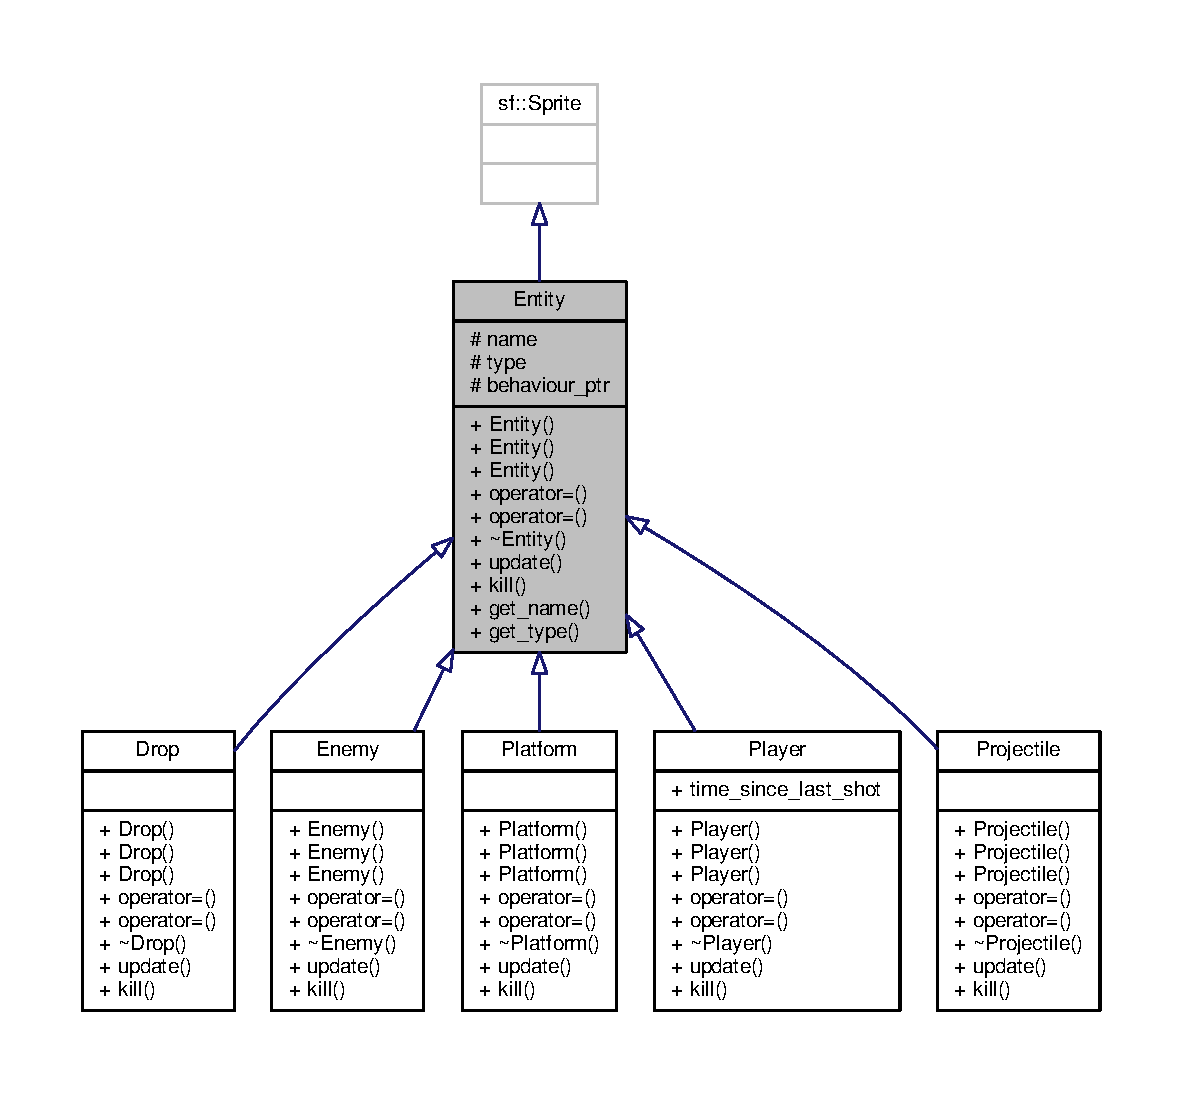
\includegraphics[width=350pt]{classEntity__inherit__graph}
\end{center}
\end{figure}


Collaboration diagram for Entity\+:\nopagebreak
\begin{figure}[H]
\begin{center}
\leavevmode
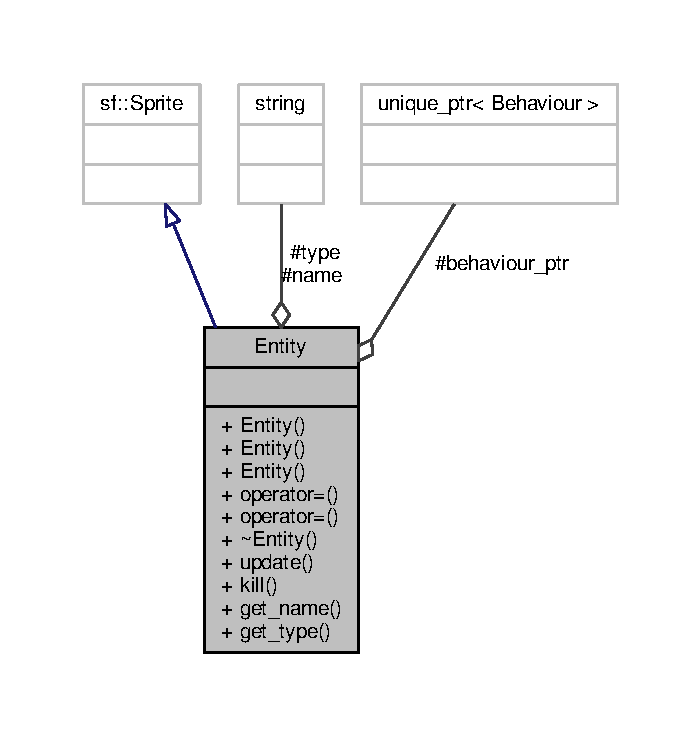
\includegraphics[width=336pt]{classEntity__coll__graph}
\end{center}
\end{figure}
\subsection*{Public Member Functions}
\begin{DoxyCompactItemize}
\item 
\hyperlink{classEntity_a832613c9d80ae6ee8b05d659e0842fbb}{Entity} (std\+::string n, std\+::string t, \hyperlink{classBehaviour}{Behaviour} $\ast$b, sf\+::\+Texture const \&texture, sf\+::\+Int\+Rect size)
\item 
\hyperlink{classEntity_a6d2e6788f8c2be303ebc2d67764f4127}{Entity} (\hyperlink{classEntity}{Entity} const \&other)=delete
\begin{DoxyCompactList}\small\item\em Copy konstruktor. \end{DoxyCompactList}\item 
\hyperlink{classEntity_a30c067e1de9094763c219fcc14c8419a}{Entity} (\hyperlink{classEntity}{Entity} \&\&other)=delete
\begin{DoxyCompactList}\small\item\em Move konstruktor. \end{DoxyCompactList}\item 
\hyperlink{classEntity}{Entity} \& \hyperlink{classEntity_a80dd8e5116a29007aef1039556d27d56}{operator=} (\hyperlink{classEntity}{Entity} const \&rhs)\&=delete
\begin{DoxyCompactList}\small\item\em Copy operator. \end{DoxyCompactList}\item 
\hyperlink{classEntity}{Entity} \& \hyperlink{classEntity_a0d03f941fda7705c726bf819d71faf6c}{operator=} (\hyperlink{classEntity}{Entity} \&\&rhs)=delete
\begin{DoxyCompactList}\small\item\em Move operator. \end{DoxyCompactList}\item 
virtual \hyperlink{classEntity_ac479d009ddde62dfb378ca0a70d81307}{$\sim$\+Entity} ()=default
\begin{DoxyCompactList}\small\item\em Default destruktor. \end{DoxyCompactList}\item 
virtual void \hyperlink{classEntity_a180102ac6695559b1f8fcf0aee747802}{update} (\hyperlink{classWorld}{World} \&, sf\+::\+Time const \&)=0
\item 
virtual void \hyperlink{classEntity_a3d585a30d7f07c50911485825f5496cd}{kill} (\hyperlink{classWorld}{World} \&)=0
\begin{DoxyCompactList}\small\item\em Om entiteten ska dö så signalerar denna funktion det till world. \end{DoxyCompactList}\item 
std\+::string \hyperlink{classEntity_a75c7e4aad3df2e053ee5b43169509534}{get\+\_\+name} () const 
\begin{DoxyCompactList}\small\item\em Returnerar namnet på entititen. \end{DoxyCompactList}\item 
std\+::string \hyperlink{classEntity_a0e9ef479c1147e21e5bcb338cb858df2}{get\+\_\+type} () const 
\begin{DoxyCompactList}\small\item\em Returnerar typen på entititen. \end{DoxyCompactList}\end{DoxyCompactItemize}
\subsection*{Protected Attributes}
\begin{DoxyCompactItemize}
\item 
std\+::string \hyperlink{classEntity_a931b21fbdebb1a5963b4bcab5df128f5}{name}
\begin{DoxyCompactList}\small\item\em Namn. \end{DoxyCompactList}\item 
std\+::string \hyperlink{classEntity_a298a9ebf2474bb00874b5ff6a0d637ef}{type}
\begin{DoxyCompactList}\small\item\em Typ. \end{DoxyCompactList}\item 
std\+::unique\+\_\+ptr$<$ \hyperlink{classBehaviour}{Behaviour} $>$ \hyperlink{classEntity_adb6e36848db24e6d48e6d295e19d3972}{behaviour\+\_\+ptr}
\begin{DoxyCompactList}\small\item\em Unik smart-\/pekare till ett objekt av \hyperlink{classBehaviour}{Behaviour} klassen. \end{DoxyCompactList}\end{DoxyCompactItemize}


\subsection{Detailed Description}
\hyperlink{classEntity}{Entity} ärver från sf\+::\+Sprite och är grundklassen för alla entiteter i spelvärlden. 

\subsection{Constructor \& Destructor Documentation}
\hypertarget{classEntity_a832613c9d80ae6ee8b05d659e0842fbb}{\index{Entity@{Entity}!Entity@{Entity}}
\index{Entity@{Entity}!Entity@{Entity}}
\subsubsection[{Entity}]{\setlength{\rightskip}{0pt plus 5cm}Entity\+::\+Entity (
\begin{DoxyParamCaption}
\item[{std\+::string}]{n, }
\item[{std\+::string}]{t, }
\item[{{\bf Behaviour} $\ast$}]{b, }
\item[{sf\+::\+Texture const \&}]{texture, }
\item[{sf\+::\+Int\+Rect}]{size}
\end{DoxyParamCaption}
)\hspace{0.3cm}{\ttfamily [inline]}}}\label{classEntity_a832613c9d80ae6ee8b05d659e0842fbb}
Entitys konstruktor baseras på sf\+::\+Sprites men tar också in ett namn, en typ, en pekare till behaviour , en textur och en storlek på texturen. \hypertarget{classEntity_a6d2e6788f8c2be303ebc2d67764f4127}{\index{Entity@{Entity}!Entity@{Entity}}
\index{Entity@{Entity}!Entity@{Entity}}
\subsubsection[{Entity}]{\setlength{\rightskip}{0pt plus 5cm}Entity\+::\+Entity (
\begin{DoxyParamCaption}
\item[{{\bf Entity} const \&}]{other}
\end{DoxyParamCaption}
)\hspace{0.3cm}{\ttfamily [delete]}}}\label{classEntity_a6d2e6788f8c2be303ebc2d67764f4127}


Copy konstruktor. 

\hypertarget{classEntity_a30c067e1de9094763c219fcc14c8419a}{\index{Entity@{Entity}!Entity@{Entity}}
\index{Entity@{Entity}!Entity@{Entity}}
\subsubsection[{Entity}]{\setlength{\rightskip}{0pt plus 5cm}Entity\+::\+Entity (
\begin{DoxyParamCaption}
\item[{{\bf Entity} \&\&}]{other}
\end{DoxyParamCaption}
)\hspace{0.3cm}{\ttfamily [delete]}}}\label{classEntity_a30c067e1de9094763c219fcc14c8419a}


Move konstruktor. 

\hypertarget{classEntity_ac479d009ddde62dfb378ca0a70d81307}{\index{Entity@{Entity}!````~Entity@{$\sim$\+Entity}}
\index{````~Entity@{$\sim$\+Entity}!Entity@{Entity}}
\subsubsection[{$\sim$\+Entity}]{\setlength{\rightskip}{0pt plus 5cm}virtual Entity\+::$\sim$\+Entity (
\begin{DoxyParamCaption}
{}
\end{DoxyParamCaption}
)\hspace{0.3cm}{\ttfamily [virtual]}, {\ttfamily [default]}}}\label{classEntity_ac479d009ddde62dfb378ca0a70d81307}


Default destruktor. 



\subsection{Member Function Documentation}
\hypertarget{classEntity_a75c7e4aad3df2e053ee5b43169509534}{\index{Entity@{Entity}!get\+\_\+name@{get\+\_\+name}}
\index{get\+\_\+name@{get\+\_\+name}!Entity@{Entity}}
\subsubsection[{get\+\_\+name}]{\setlength{\rightskip}{0pt plus 5cm}std\+::string Entity\+::get\+\_\+name (
\begin{DoxyParamCaption}
{}
\end{DoxyParamCaption}
) const\hspace{0.3cm}{\ttfamily [inline]}}}\label{classEntity_a75c7e4aad3df2e053ee5b43169509534}


Returnerar namnet på entititen. 

\hypertarget{classEntity_a0e9ef479c1147e21e5bcb338cb858df2}{\index{Entity@{Entity}!get\+\_\+type@{get\+\_\+type}}
\index{get\+\_\+type@{get\+\_\+type}!Entity@{Entity}}
\subsubsection[{get\+\_\+type}]{\setlength{\rightskip}{0pt plus 5cm}std\+::string Entity\+::get\+\_\+type (
\begin{DoxyParamCaption}
{}
\end{DoxyParamCaption}
) const\hspace{0.3cm}{\ttfamily [inline]}}}\label{classEntity_a0e9ef479c1147e21e5bcb338cb858df2}


Returnerar typen på entititen. 

\hypertarget{classEntity_a3d585a30d7f07c50911485825f5496cd}{\index{Entity@{Entity}!kill@{kill}}
\index{kill@{kill}!Entity@{Entity}}
\subsubsection[{kill}]{\setlength{\rightskip}{0pt plus 5cm}virtual void Entity\+::kill (
\begin{DoxyParamCaption}
\item[{{\bf World} \&}]{}
\end{DoxyParamCaption}
)\hspace{0.3cm}{\ttfamily [pure virtual]}}}\label{classEntity_a3d585a30d7f07c50911485825f5496cd}


Om entiteten ska dö så signalerar denna funktion det till world. 



Implemented in \hyperlink{classEnemy_aba8130fd5f8ede411cded7611254ab7a}{Enemy}, \hyperlink{classDrop_a8bbd94b3140a246297aaf4c984dad4ee}{Drop}, \hyperlink{classPlatform_a6dd2fe10f6de044db339c5050bdb7ef0}{Platform}, \hyperlink{classProjectile_a10d7ca9bb3d022246196572d008f1d59}{Projectile}, and \hyperlink{classPlayer_ab015823a5707509c3611ff93984100d9}{Player}.

\hypertarget{classEntity_a80dd8e5116a29007aef1039556d27d56}{\index{Entity@{Entity}!operator=@{operator=}}
\index{operator=@{operator=}!Entity@{Entity}}
\subsubsection[{operator=}]{\setlength{\rightskip}{0pt plus 5cm}{\bf Entity}\& Entity\+::operator= (
\begin{DoxyParamCaption}
\item[{{\bf Entity} const \&}]{rhs}
\end{DoxyParamCaption}
)\hspace{0.3cm}{\ttfamily [delete]}}}\label{classEntity_a80dd8e5116a29007aef1039556d27d56}


Copy operator. 

\hypertarget{classEntity_a0d03f941fda7705c726bf819d71faf6c}{\index{Entity@{Entity}!operator=@{operator=}}
\index{operator=@{operator=}!Entity@{Entity}}
\subsubsection[{operator=}]{\setlength{\rightskip}{0pt plus 5cm}{\bf Entity}\& Entity\+::operator= (
\begin{DoxyParamCaption}
\item[{{\bf Entity} \&\&}]{rhs}
\end{DoxyParamCaption}
)\hspace{0.3cm}{\ttfamily [delete]}}}\label{classEntity_a0d03f941fda7705c726bf819d71faf6c}


Move operator. 

\hypertarget{classEntity_a180102ac6695559b1f8fcf0aee747802}{\index{Entity@{Entity}!update@{update}}
\index{update@{update}!Entity@{Entity}}
\subsubsection[{update}]{\setlength{\rightskip}{0pt plus 5cm}virtual void Entity\+::update (
\begin{DoxyParamCaption}
\item[{{\bf World} \&}]{, }
\item[{sf\+::\+Time const \&}]{}
\end{DoxyParamCaption}
)\hspace{0.3cm}{\ttfamily [pure virtual]}}}\label{classEntity_a180102ac6695559b1f8fcf0aee747802}
Funktionen som world kallar på för att få varje entitet att uppdatera sig. Den kallar i sin tur på Behaviour\+::\+Process() 

Implemented in \hyperlink{classEnemy_a257cacd04930ccbfa9545bb5a8dc5be3}{Enemy}, \hyperlink{classDrop_aa899493774d2a66cbb51f3cd9a0cf80e}{Drop}, \hyperlink{classPlatform_ad756e0494312cdd8956af8bee6afbb0f}{Platform}, \hyperlink{classProjectile_a48d52d5d9db6e3af4aae8ded6afa6544}{Projectile}, and \hyperlink{classPlayer_ad0f6610ee4a9f6d179bf404d1812be54}{Player}.



\subsection{Member Data Documentation}
\hypertarget{classEntity_adb6e36848db24e6d48e6d295e19d3972}{\index{Entity@{Entity}!behaviour\+\_\+ptr@{behaviour\+\_\+ptr}}
\index{behaviour\+\_\+ptr@{behaviour\+\_\+ptr}!Entity@{Entity}}
\subsubsection[{behaviour\+\_\+ptr}]{\setlength{\rightskip}{0pt plus 5cm}std\+::unique\+\_\+ptr$<${\bf Behaviour}$>$ Entity\+::behaviour\+\_\+ptr\hspace{0.3cm}{\ttfamily [protected]}}}\label{classEntity_adb6e36848db24e6d48e6d295e19d3972}


Unik smart-\/pekare till ett objekt av \hyperlink{classBehaviour}{Behaviour} klassen. 

\hypertarget{classEntity_a931b21fbdebb1a5963b4bcab5df128f5}{\index{Entity@{Entity}!name@{name}}
\index{name@{name}!Entity@{Entity}}
\subsubsection[{name}]{\setlength{\rightskip}{0pt plus 5cm}std\+::string Entity\+::name\hspace{0.3cm}{\ttfamily [protected]}}}\label{classEntity_a931b21fbdebb1a5963b4bcab5df128f5}


Namn. 

\hypertarget{classEntity_a298a9ebf2474bb00874b5ff6a0d637ef}{\index{Entity@{Entity}!type@{type}}
\index{type@{type}!Entity@{Entity}}
\subsubsection[{type}]{\setlength{\rightskip}{0pt plus 5cm}std\+::string Entity\+::type\hspace{0.3cm}{\ttfamily [protected]}}}\label{classEntity_a298a9ebf2474bb00874b5ff6a0d637ef}


Typ. 



The documentation for this class was generated from the following file\+:\begin{DoxyCompactItemize}
\item 
source/objects/headers/Entity.\+h\end{DoxyCompactItemize}

\hypertarget{classGame}{\section{Game Class Reference}
\label{classGame}\index{Game@{Game}}
}


\hyperlink{classGame}{Game} som kör spelvärlden och har hand om main loopen.  




{\ttfamily \#include $<$Game.\+h$>$}



Collaboration diagram for Game\+:\nopagebreak
\begin{figure}[H]
\begin{center}
\leavevmode
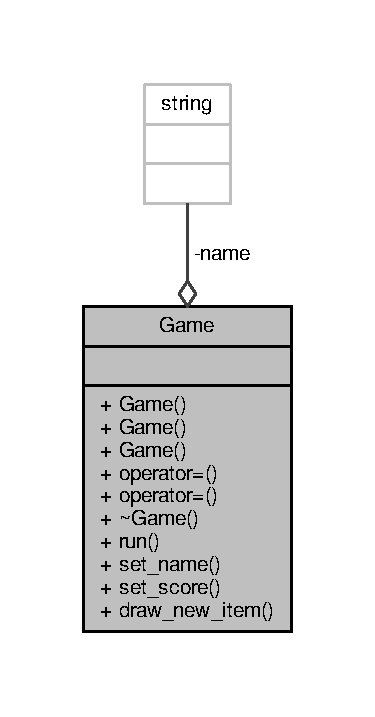
\includegraphics[width=180pt]{classGame__coll__graph}
\end{center}
\end{figure}
\subsection*{Public Member Functions}
\begin{DoxyCompactItemize}
\item 
\hyperlink{classGame_a4735989677c1cab18866f3ae4ee0aa1c}{Game} ()=default
\begin{DoxyCompactList}\small\item\em Default konstruktor. \end{DoxyCompactList}\item 
\hyperlink{classGame_a09c8ffcbf57e2e60f86a4c6071c73df1}{Game} (\hyperlink{classGame}{Game} const \&other)=delete
\begin{DoxyCompactList}\small\item\em Copy konstruktor. \end{DoxyCompactList}\item 
\hyperlink{classGame_af6029629f9ebfc665b355daa0ba5702b}{Game} (\hyperlink{classGame}{Game} \&\&other)=delete
\begin{DoxyCompactList}\small\item\em Move konstruktor. \end{DoxyCompactList}\item 
\hyperlink{classGame}{Game} \& \hyperlink{classGame_a3679df3694806d8d8580d7ac8a351300}{operator=} (\hyperlink{classGame}{Game} const \&rhs)\&=delete
\begin{DoxyCompactList}\small\item\em Copy operator. \end{DoxyCompactList}\item 
\hyperlink{classGame}{Game} \& \hyperlink{classGame_a059b8ac540d33c882ae792f9590cc93c}{operator=} (\hyperlink{classGame}{Game} \&\&rhs)=delete
\begin{DoxyCompactList}\small\item\em Move operator. \end{DoxyCompactList}\item 
\hyperlink{classGame_a3d09cd0b68ef69107d36360ca903e023}{$\sim$\+Game} ()=default
\begin{DoxyCompactList}\small\item\em Default destruktor. \end{DoxyCompactList}\item 
int \hyperlink{classGame_aedc2d87ef2e375e019c4c6f3d47da429}{run} (int)
\begin{DoxyCompactList}\small\item\em Funktionen som kör själva spelet. \end{DoxyCompactList}\item 
void \hyperlink{classGame_a7dd41abdb2a4d0c72f328e1035b2cd06}{set\+\_\+name} (std\+::string)
\begin{DoxyCompactList}\small\item\em Sätter spelarens namn. \end{DoxyCompactList}\item 
void \hyperlink{classGame_a0626eca623682fa3f6b925656e790214}{set\+\_\+score} (\hyperlink{classWorld}{World} \&)
\begin{DoxyCompactList}\small\item\em Skriver spelarens score till en .txt fil. \end{DoxyCompactList}\item 
void \hyperlink{classGame_ad0c6cacf0ac2063f5e0e169a46adcdb7}{draw\+\_\+new\+\_\+item} (std\+::string const \&, sf\+::\+Vector2f const \&, sf\+::\+Font const \&, sf\+::\+Render\+Window \&)
\end{DoxyCompactItemize}
\subsection*{Private Attributes}
\begin{DoxyCompactItemize}
\item 
std\+::string \hyperlink{classGame_a7f9c64d3f7fd7694c544b4c68d72569d}{name} \{\char`\"{}Player\char`\"{}\}
\begin{DoxyCompactList}\small\item\em Variabel för spelarens namn. \end{DoxyCompactList}\end{DoxyCompactItemize}


\subsection{Detailed Description}
\hyperlink{classGame}{Game} som kör spelvärlden och har hand om main loopen. 

\hyperlink{classGame}{Game} hanterar main loopen i sin \hyperlink{classGame_aedc2d87ef2e375e019c4c6f3d47da429}{Game\+::run()} och skapar där \hyperlink{classWorld}{World} objektet och \hyperlink{classLevel}{Level} Objektet. Sedan håller den koll på när \hyperlink{classKey__Handling}{Key\+\_\+\+Handling} ska få knapptryckningar, när allt ska uppdateras genom \hyperlink{classWorld_abe8efb7955edd02cfdae5f99f2e5a346}{World\+::update\+\_\+all()} och när allt ska ritas ut med \hyperlink{classWorld_a56d3640e46fef8b3e62538f067e2fbd2}{World\+::render\+\_\+all()} och sfml sf\+::\+Render\+Window.\+display(). Den skapar också dödsskärmen och skriver in high score efter att spelaren har dött. 

\subsection{Constructor \& Destructor Documentation}
\hypertarget{classGame_a4735989677c1cab18866f3ae4ee0aa1c}{\index{Game@{Game}!Game@{Game}}
\index{Game@{Game}!Game@{Game}}
\subsubsection[{Game}]{\setlength{\rightskip}{0pt plus 5cm}Game\+::\+Game (
\begin{DoxyParamCaption}
{}
\end{DoxyParamCaption}
)\hspace{0.3cm}{\ttfamily [default]}}}\label{classGame_a4735989677c1cab18866f3ae4ee0aa1c}


Default konstruktor. 

\hypertarget{classGame_a09c8ffcbf57e2e60f86a4c6071c73df1}{\index{Game@{Game}!Game@{Game}}
\index{Game@{Game}!Game@{Game}}
\subsubsection[{Game}]{\setlength{\rightskip}{0pt plus 5cm}Game\+::\+Game (
\begin{DoxyParamCaption}
\item[{{\bf Game} const \&}]{other}
\end{DoxyParamCaption}
)\hspace{0.3cm}{\ttfamily [delete]}}}\label{classGame_a09c8ffcbf57e2e60f86a4c6071c73df1}


Copy konstruktor. 

\hypertarget{classGame_af6029629f9ebfc665b355daa0ba5702b}{\index{Game@{Game}!Game@{Game}}
\index{Game@{Game}!Game@{Game}}
\subsubsection[{Game}]{\setlength{\rightskip}{0pt plus 5cm}Game\+::\+Game (
\begin{DoxyParamCaption}
\item[{{\bf Game} \&\&}]{other}
\end{DoxyParamCaption}
)\hspace{0.3cm}{\ttfamily [delete]}}}\label{classGame_af6029629f9ebfc665b355daa0ba5702b}


Move konstruktor. 

\hypertarget{classGame_a3d09cd0b68ef69107d36360ca903e023}{\index{Game@{Game}!````~Game@{$\sim$\+Game}}
\index{````~Game@{$\sim$\+Game}!Game@{Game}}
\subsubsection[{$\sim$\+Game}]{\setlength{\rightskip}{0pt plus 5cm}Game\+::$\sim$\+Game (
\begin{DoxyParamCaption}
{}
\end{DoxyParamCaption}
)\hspace{0.3cm}{\ttfamily [default]}}}\label{classGame_a3d09cd0b68ef69107d36360ca903e023}


Default destruktor. 



\subsection{Member Function Documentation}
\hypertarget{classGame_ad0c6cacf0ac2063f5e0e169a46adcdb7}{\index{Game@{Game}!draw\+\_\+new\+\_\+item@{draw\+\_\+new\+\_\+item}}
\index{draw\+\_\+new\+\_\+item@{draw\+\_\+new\+\_\+item}!Game@{Game}}
\subsubsection[{draw\+\_\+new\+\_\+item}]{\setlength{\rightskip}{0pt plus 5cm}void Game\+::draw\+\_\+new\+\_\+item (
\begin{DoxyParamCaption}
\item[{std\+::string const \&}]{s, }
\item[{sf\+::\+Vector2f const \&}]{v, }
\item[{sf\+::\+Font const \&}]{f, }
\item[{sf\+::\+Render\+Window \&}]{window}
\end{DoxyParamCaption}
)}}\label{classGame_ad0c6cacf0ac2063f5e0e169a46adcdb7}
Funktion som ritar ut ett objekt på spelplanen som inte är en del av spelet. T.\+ex. antal liv, score och pausskärmen. \hypertarget{classGame_a3679df3694806d8d8580d7ac8a351300}{\index{Game@{Game}!operator=@{operator=}}
\index{operator=@{operator=}!Game@{Game}}
\subsubsection[{operator=}]{\setlength{\rightskip}{0pt plus 5cm}{\bf Game}\& Game\+::operator= (
\begin{DoxyParamCaption}
\item[{{\bf Game} const \&}]{rhs}
\end{DoxyParamCaption}
)\hspace{0.3cm}{\ttfamily [delete]}}}\label{classGame_a3679df3694806d8d8580d7ac8a351300}


Copy operator. 

\hypertarget{classGame_a059b8ac540d33c882ae792f9590cc93c}{\index{Game@{Game}!operator=@{operator=}}
\index{operator=@{operator=}!Game@{Game}}
\subsubsection[{operator=}]{\setlength{\rightskip}{0pt plus 5cm}{\bf Game}\& Game\+::operator= (
\begin{DoxyParamCaption}
\item[{{\bf Game} \&\&}]{rhs}
\end{DoxyParamCaption}
)\hspace{0.3cm}{\ttfamily [delete]}}}\label{classGame_a059b8ac540d33c882ae792f9590cc93c}


Move operator. 

\hypertarget{classGame_aedc2d87ef2e375e019c4c6f3d47da429}{\index{Game@{Game}!run@{run}}
\index{run@{run}!Game@{Game}}
\subsubsection[{run}]{\setlength{\rightskip}{0pt plus 5cm}int Game\+::run (
\begin{DoxyParamCaption}
\item[{int}]{player\+\_\+amount}
\end{DoxyParamCaption}
)}}\label{classGame_aedc2d87ef2e375e019c4c6f3d47da429}


Funktionen som kör själva spelet. 

\hypertarget{classGame_a7dd41abdb2a4d0c72f328e1035b2cd06}{\index{Game@{Game}!set\+\_\+name@{set\+\_\+name}}
\index{set\+\_\+name@{set\+\_\+name}!Game@{Game}}
\subsubsection[{set\+\_\+name}]{\setlength{\rightskip}{0pt plus 5cm}void Game\+::set\+\_\+name (
\begin{DoxyParamCaption}
\item[{std\+::string}]{n}
\end{DoxyParamCaption}
)}}\label{classGame_a7dd41abdb2a4d0c72f328e1035b2cd06}


Sätter spelarens namn. 

\hypertarget{classGame_a0626eca623682fa3f6b925656e790214}{\index{Game@{Game}!set\+\_\+score@{set\+\_\+score}}
\index{set\+\_\+score@{set\+\_\+score}!Game@{Game}}
\subsubsection[{set\+\_\+score}]{\setlength{\rightskip}{0pt plus 5cm}void Game\+::set\+\_\+score (
\begin{DoxyParamCaption}
\item[{{\bf World} \&}]{w}
\end{DoxyParamCaption}
)}}\label{classGame_a0626eca623682fa3f6b925656e790214}


Skriver spelarens score till en .txt fil. 



\subsection{Member Data Documentation}
\hypertarget{classGame_a7f9c64d3f7fd7694c544b4c68d72569d}{\index{Game@{Game}!name@{name}}
\index{name@{name}!Game@{Game}}
\subsubsection[{name}]{\setlength{\rightskip}{0pt plus 5cm}std\+::string Game\+::name \{\char`\"{}Player\char`\"{}\}\hspace{0.3cm}{\ttfamily [private]}}}\label{classGame_a7f9c64d3f7fd7694c544b4c68d72569d}


Variabel för spelarens namn. 



The documentation for this class was generated from the following files\+:\begin{DoxyCompactItemize}
\item 
source/objects/headers/Game.\+h\item 
source/objects/imps/Game.\+cpp\end{DoxyCompactItemize}

\hypertarget{classKey__Handling}{\section{Key\+\_\+\+Handling Class Reference}
\label{classKey__Handling}\index{Key\+\_\+\+Handling@{Key\+\_\+\+Handling}}
}


\hyperlink{classKey__Handling}{Key\+\_\+\+Handling} har hand om input från spelaren.  




{\ttfamily \#include $<$Key\+\_\+\+Handling.\+h$>$}



Collaboration diagram for Key\+\_\+\+Handling\+:\nopagebreak
\begin{figure}[H]
\begin{center}
\leavevmode
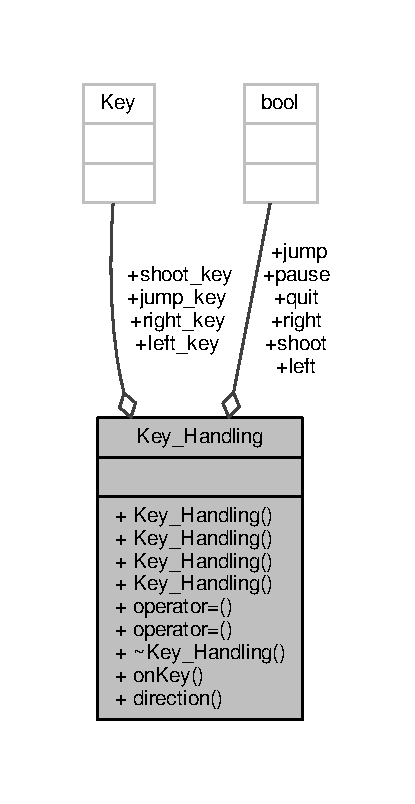
\includegraphics[width=199pt]{classKey__Handling__coll__graph}
\end{center}
\end{figure}
\subsection*{Public Member Functions}
\begin{DoxyCompactItemize}
\item 
\hyperlink{classKey__Handling_ad39f9645a4c3b4a91c9116e96afd55d8}{Key\+\_\+\+Handling} ()
\begin{DoxyCompactList}\small\item\em Default konstruktor som skapar \hyperlink{classKey__Handling}{Key\+\_\+\+Handling} med fördefinierade tangenter. \end{DoxyCompactList}\item 
\hyperlink{classKey__Handling_a8fc595ca2ab4cf2c542ca36fd1d34b15}{Key\+\_\+\+Handling} (sf\+::\+Keyboard\+::\+Key, sf\+::\+Keyboard\+::\+Key, sf\+::\+Keyboard\+::\+Key, sf\+::\+Keyboard\+::\+Key)
\begin{DoxyCompactList}\small\item\em Konstruktor som tar emot 4 tangenter. \end{DoxyCompactList}\item 
\hyperlink{classKey__Handling_a77ab751460e13501b55aa602195fd164}{Key\+\_\+\+Handling} (\hyperlink{classKey__Handling}{Key\+\_\+\+Handling} const \&other)=delete
\begin{DoxyCompactList}\small\item\em Copy konstruktor. \end{DoxyCompactList}\item 
\hyperlink{classKey__Handling_afcba70ccd67070d27370c808bf14f26b}{Key\+\_\+\+Handling} (\hyperlink{classKey__Handling}{Key\+\_\+\+Handling} \&\&other)=delete
\begin{DoxyCompactList}\small\item\em Move konstruktor. \end{DoxyCompactList}\item 
\hyperlink{classKey__Handling}{Key\+\_\+\+Handling} \& \hyperlink{classKey__Handling_aa8c89a0450a74fc1888089d568c2e87f}{operator=} (\hyperlink{classKey__Handling}{Key\+\_\+\+Handling} const \&rhs)\&=delete
\begin{DoxyCompactList}\small\item\em Copy operator. \end{DoxyCompactList}\item 
\hyperlink{classKey__Handling}{Key\+\_\+\+Handling} \& \hyperlink{classKey__Handling_a095581108c0abb43b0f6c9a67cc62f54}{operator=} (\hyperlink{classKey__Handling}{Key\+\_\+\+Handling} \&\&rhs)=delete
\begin{DoxyCompactList}\small\item\em Move operator. \end{DoxyCompactList}\item 
\hyperlink{classKey__Handling_abaeb9c9b746106e475c8d91743271cab}{$\sim$\+Key\+\_\+\+Handling} ()=default
\begin{DoxyCompactList}\small\item\em Default destruktor. \end{DoxyCompactList}\item 
void \hyperlink{classKey__Handling_a44d85d656914e718a9b155c41d687771}{on\+Key} (bool, sf\+::\+Keyboard\+::\+Key const \&)
\item 
sf\+::\+Vector2f \hyperlink{classKey__Handling_adaea1f1ba27262539509061cbc818361}{direction} () const 
\end{DoxyCompactItemize}
\subsection*{Public Attributes}
\begin{DoxyCompactItemize}
\item 
bool \hyperlink{classKey__Handling_af7bf77c8b1d7ed6ea3282f45f76fcf61}{jump} \{false\}
\begin{DoxyCompactList}\small\item\em Variabel för hopp knappen. \end{DoxyCompactList}\item 
bool \hyperlink{classKey__Handling_ab72108363edad52be4d7c4d8a572f6ec}{left} \{false\}
\begin{DoxyCompactList}\small\item\em Variabel för vänster movement. \end{DoxyCompactList}\item 
bool \hyperlink{classKey__Handling_a494ba1ae43c55d5202f24e9bc78c5ed1}{right} \{false\}
\begin{DoxyCompactList}\small\item\em Variabel för höger movement. \end{DoxyCompactList}\item 
bool \hyperlink{classKey__Handling_ae9d219c1a9387620c14120d9a45d5db1}{shoot} \{false\}
\begin{DoxyCompactList}\small\item\em Variabel för att skjuta. \end{DoxyCompactList}\item 
bool \hyperlink{classKey__Handling_a73a615e629c4d3db0bbecb6fd35fe31b}{quit} \{false\}
\begin{DoxyCompactList}\small\item\em Variabel för att avsluta spelet. \end{DoxyCompactList}\item 
bool \hyperlink{classKey__Handling_ae297ccc0a53483abe41f2788ec7863d8}{pause} \{false\}
\begin{DoxyCompactList}\small\item\em Variabel för att pausa spelet. \end{DoxyCompactList}\item 
sf\+::\+Keyboard\+::\+Key \hyperlink{classKey__Handling_a6d7d9bb4dc72122fc257d0a98b8613d5}{jump\+\_\+key} \{\}
\begin{DoxyCompactList}\small\item\em Variabel för vilken tangent som betyder hoppa. \end{DoxyCompactList}\item 
sf\+::\+Keyboard\+::\+Key \hyperlink{classKey__Handling_a53493a34a4c7948354017b34fc9406fa}{left\+\_\+key} \{\}
\begin{DoxyCompactList}\small\item\em Variabel för vilken tangent som betyder vänster. \end{DoxyCompactList}\item 
sf\+::\+Keyboard\+::\+Key \hyperlink{classKey__Handling_a802f80c79ced68d848e1297438c1627e}{right\+\_\+key} \{\}
\begin{DoxyCompactList}\small\item\em Variabel för vilken tangent som betyder höger. \end{DoxyCompactList}\item 
sf\+::\+Keyboard\+::\+Key \hyperlink{classKey__Handling_a73d59e5daa95dc140adda8cfd677e189}{shoot\+\_\+key} \{\}
\begin{DoxyCompactList}\small\item\em Variabel för vilken tangent som betyder skjut. \end{DoxyCompactList}\end{DoxyCompactItemize}


\subsection{Detailed Description}
\hyperlink{classKey__Handling}{Key\+\_\+\+Handling} har hand om input från spelaren. 

\hyperlink{classKey__Handling}{Key\+\_\+\+Handling} är den klass som tar hand om tangenttryckningar. Den gör detta genom att ta emot S\+F\+M\+Ls Keyboard structs. Den kollar vilka tangenter som tryckts ner och ändrar sedan \hyperlink{classKey__Handling_adaea1f1ba27262539509061cbc818361}{Key\+\_\+\+Handling\+::direction()} för att visa vad som har tryckts ner. Det går också att kolla direkt mot denna då den är publik om det är en knapp som inte har med movement att göra t.\+ex. \hyperlink{classKey__Handling_ae9d219c1a9387620c14120d9a45d5db1}{Key\+\_\+\+Handling\+::shoot} eller \hyperlink{classKey__Handling_a73a615e629c4d3db0bbecb6fd35fe31b}{Key\+\_\+\+Handling\+::quit}. 

\subsection{Constructor \& Destructor Documentation}
\hypertarget{classKey__Handling_ad39f9645a4c3b4a91c9116e96afd55d8}{\index{Key\+\_\+\+Handling@{Key\+\_\+\+Handling}!Key\+\_\+\+Handling@{Key\+\_\+\+Handling}}
\index{Key\+\_\+\+Handling@{Key\+\_\+\+Handling}!Key\+\_\+\+Handling@{Key\+\_\+\+Handling}}
\subsubsection[{Key\+\_\+\+Handling}]{\setlength{\rightskip}{0pt plus 5cm}Key\+\_\+\+Handling\+::\+Key\+\_\+\+Handling (
\begin{DoxyParamCaption}
{}
\end{DoxyParamCaption}
)}}\label{classKey__Handling_ad39f9645a4c3b4a91c9116e96afd55d8}


Default konstruktor som skapar \hyperlink{classKey__Handling}{Key\+\_\+\+Handling} med fördefinierade tangenter. 

\hypertarget{classKey__Handling_a8fc595ca2ab4cf2c542ca36fd1d34b15}{\index{Key\+\_\+\+Handling@{Key\+\_\+\+Handling}!Key\+\_\+\+Handling@{Key\+\_\+\+Handling}}
\index{Key\+\_\+\+Handling@{Key\+\_\+\+Handling}!Key\+\_\+\+Handling@{Key\+\_\+\+Handling}}
\subsubsection[{Key\+\_\+\+Handling}]{\setlength{\rightskip}{0pt plus 5cm}Key\+\_\+\+Handling\+::\+Key\+\_\+\+Handling (
\begin{DoxyParamCaption}
\item[{sf\+::\+Keyboard\+::\+Key}]{j, }
\item[{sf\+::\+Keyboard\+::\+Key}]{l, }
\item[{sf\+::\+Keyboard\+::\+Key}]{r, }
\item[{sf\+::\+Keyboard\+::\+Key}]{s}
\end{DoxyParamCaption}
)}}\label{classKey__Handling_a8fc595ca2ab4cf2c542ca36fd1d34b15}


Konstruktor som tar emot 4 tangenter. 

\hypertarget{classKey__Handling_a77ab751460e13501b55aa602195fd164}{\index{Key\+\_\+\+Handling@{Key\+\_\+\+Handling}!Key\+\_\+\+Handling@{Key\+\_\+\+Handling}}
\index{Key\+\_\+\+Handling@{Key\+\_\+\+Handling}!Key\+\_\+\+Handling@{Key\+\_\+\+Handling}}
\subsubsection[{Key\+\_\+\+Handling}]{\setlength{\rightskip}{0pt plus 5cm}Key\+\_\+\+Handling\+::\+Key\+\_\+\+Handling (
\begin{DoxyParamCaption}
\item[{{\bf Key\+\_\+\+Handling} const \&}]{other}
\end{DoxyParamCaption}
)\hspace{0.3cm}{\ttfamily [delete]}}}\label{classKey__Handling_a77ab751460e13501b55aa602195fd164}


Copy konstruktor. 

\hypertarget{classKey__Handling_afcba70ccd67070d27370c808bf14f26b}{\index{Key\+\_\+\+Handling@{Key\+\_\+\+Handling}!Key\+\_\+\+Handling@{Key\+\_\+\+Handling}}
\index{Key\+\_\+\+Handling@{Key\+\_\+\+Handling}!Key\+\_\+\+Handling@{Key\+\_\+\+Handling}}
\subsubsection[{Key\+\_\+\+Handling}]{\setlength{\rightskip}{0pt plus 5cm}Key\+\_\+\+Handling\+::\+Key\+\_\+\+Handling (
\begin{DoxyParamCaption}
\item[{{\bf Key\+\_\+\+Handling} \&\&}]{other}
\end{DoxyParamCaption}
)\hspace{0.3cm}{\ttfamily [delete]}}}\label{classKey__Handling_afcba70ccd67070d27370c808bf14f26b}


Move konstruktor. 

\hypertarget{classKey__Handling_abaeb9c9b746106e475c8d91743271cab}{\index{Key\+\_\+\+Handling@{Key\+\_\+\+Handling}!````~Key\+\_\+\+Handling@{$\sim$\+Key\+\_\+\+Handling}}
\index{````~Key\+\_\+\+Handling@{$\sim$\+Key\+\_\+\+Handling}!Key\+\_\+\+Handling@{Key\+\_\+\+Handling}}
\subsubsection[{$\sim$\+Key\+\_\+\+Handling}]{\setlength{\rightskip}{0pt plus 5cm}Key\+\_\+\+Handling\+::$\sim$\+Key\+\_\+\+Handling (
\begin{DoxyParamCaption}
{}
\end{DoxyParamCaption}
)\hspace{0.3cm}{\ttfamily [default]}}}\label{classKey__Handling_abaeb9c9b746106e475c8d91743271cab}


Default destruktor. 



\subsection{Member Function Documentation}
\hypertarget{classKey__Handling_adaea1f1ba27262539509061cbc818361}{\index{Key\+\_\+\+Handling@{Key\+\_\+\+Handling}!direction@{direction}}
\index{direction@{direction}!Key\+\_\+\+Handling@{Key\+\_\+\+Handling}}
\subsubsection[{direction}]{\setlength{\rightskip}{0pt plus 5cm}sf\+::\+Vector2f Key\+\_\+\+Handling\+::direction (
\begin{DoxyParamCaption}
{}
\end{DoxyParamCaption}
) const}}\label{classKey__Handling_adaea1f1ba27262539509061cbc818361}
En funktion som tillhandahåller en sf\+::\+Vector2f baserat på vilka knappar som trycks ner när funktionen kallas på. \hypertarget{classKey__Handling_a44d85d656914e718a9b155c41d687771}{\index{Key\+\_\+\+Handling@{Key\+\_\+\+Handling}!on\+Key@{on\+Key}}
\index{on\+Key@{on\+Key}!Key\+\_\+\+Handling@{Key\+\_\+\+Handling}}
\subsubsection[{on\+Key}]{\setlength{\rightskip}{0pt plus 5cm}void Key\+\_\+\+Handling\+::on\+Key (
\begin{DoxyParamCaption}
\item[{bool}]{pressed, }
\item[{sf\+::\+Keyboard\+::\+Key const \&}]{key}
\end{DoxyParamCaption}
)}}\label{classKey__Handling_a44d85d656914e718a9b155c41d687771}
Funktion som körs från main-\/loopen. Den tar emot huruvida tangenten släpptes eller trycktes ner och vilken tangent det var som triggrade eventet. \hypertarget{classKey__Handling_aa8c89a0450a74fc1888089d568c2e87f}{\index{Key\+\_\+\+Handling@{Key\+\_\+\+Handling}!operator=@{operator=}}
\index{operator=@{operator=}!Key\+\_\+\+Handling@{Key\+\_\+\+Handling}}
\subsubsection[{operator=}]{\setlength{\rightskip}{0pt plus 5cm}{\bf Key\+\_\+\+Handling}\& Key\+\_\+\+Handling\+::operator= (
\begin{DoxyParamCaption}
\item[{{\bf Key\+\_\+\+Handling} const \&}]{rhs}
\end{DoxyParamCaption}
)\hspace{0.3cm}{\ttfamily [delete]}}}\label{classKey__Handling_aa8c89a0450a74fc1888089d568c2e87f}


Copy operator. 

\hypertarget{classKey__Handling_a095581108c0abb43b0f6c9a67cc62f54}{\index{Key\+\_\+\+Handling@{Key\+\_\+\+Handling}!operator=@{operator=}}
\index{operator=@{operator=}!Key\+\_\+\+Handling@{Key\+\_\+\+Handling}}
\subsubsection[{operator=}]{\setlength{\rightskip}{0pt plus 5cm}{\bf Key\+\_\+\+Handling}\& Key\+\_\+\+Handling\+::operator= (
\begin{DoxyParamCaption}
\item[{{\bf Key\+\_\+\+Handling} \&\&}]{rhs}
\end{DoxyParamCaption}
)\hspace{0.3cm}{\ttfamily [delete]}}}\label{classKey__Handling_a095581108c0abb43b0f6c9a67cc62f54}


Move operator. 



\subsection{Member Data Documentation}
\hypertarget{classKey__Handling_af7bf77c8b1d7ed6ea3282f45f76fcf61}{\index{Key\+\_\+\+Handling@{Key\+\_\+\+Handling}!jump@{jump}}
\index{jump@{jump}!Key\+\_\+\+Handling@{Key\+\_\+\+Handling}}
\subsubsection[{jump}]{\setlength{\rightskip}{0pt plus 5cm}bool Key\+\_\+\+Handling\+::jump \{false\}}}\label{classKey__Handling_af7bf77c8b1d7ed6ea3282f45f76fcf61}


Variabel för hopp knappen. 

\hypertarget{classKey__Handling_a6d7d9bb4dc72122fc257d0a98b8613d5}{\index{Key\+\_\+\+Handling@{Key\+\_\+\+Handling}!jump\+\_\+key@{jump\+\_\+key}}
\index{jump\+\_\+key@{jump\+\_\+key}!Key\+\_\+\+Handling@{Key\+\_\+\+Handling}}
\subsubsection[{jump\+\_\+key}]{\setlength{\rightskip}{0pt plus 5cm}sf\+::\+Keyboard\+::\+Key Key\+\_\+\+Handling\+::jump\+\_\+key \{\}}}\label{classKey__Handling_a6d7d9bb4dc72122fc257d0a98b8613d5}


Variabel för vilken tangent som betyder hoppa. 

\hypertarget{classKey__Handling_ab72108363edad52be4d7c4d8a572f6ec}{\index{Key\+\_\+\+Handling@{Key\+\_\+\+Handling}!left@{left}}
\index{left@{left}!Key\+\_\+\+Handling@{Key\+\_\+\+Handling}}
\subsubsection[{left}]{\setlength{\rightskip}{0pt plus 5cm}bool Key\+\_\+\+Handling\+::left \{false\}}}\label{classKey__Handling_ab72108363edad52be4d7c4d8a572f6ec}


Variabel för vänster movement. 

\hypertarget{classKey__Handling_a53493a34a4c7948354017b34fc9406fa}{\index{Key\+\_\+\+Handling@{Key\+\_\+\+Handling}!left\+\_\+key@{left\+\_\+key}}
\index{left\+\_\+key@{left\+\_\+key}!Key\+\_\+\+Handling@{Key\+\_\+\+Handling}}
\subsubsection[{left\+\_\+key}]{\setlength{\rightskip}{0pt plus 5cm}sf\+::\+Keyboard\+::\+Key Key\+\_\+\+Handling\+::left\+\_\+key \{\}}}\label{classKey__Handling_a53493a34a4c7948354017b34fc9406fa}


Variabel för vilken tangent som betyder vänster. 

\hypertarget{classKey__Handling_ae297ccc0a53483abe41f2788ec7863d8}{\index{Key\+\_\+\+Handling@{Key\+\_\+\+Handling}!pause@{pause}}
\index{pause@{pause}!Key\+\_\+\+Handling@{Key\+\_\+\+Handling}}
\subsubsection[{pause}]{\setlength{\rightskip}{0pt plus 5cm}bool Key\+\_\+\+Handling\+::pause \{false\}}}\label{classKey__Handling_ae297ccc0a53483abe41f2788ec7863d8}


Variabel för att pausa spelet. 

\hypertarget{classKey__Handling_a73a615e629c4d3db0bbecb6fd35fe31b}{\index{Key\+\_\+\+Handling@{Key\+\_\+\+Handling}!quit@{quit}}
\index{quit@{quit}!Key\+\_\+\+Handling@{Key\+\_\+\+Handling}}
\subsubsection[{quit}]{\setlength{\rightskip}{0pt plus 5cm}bool Key\+\_\+\+Handling\+::quit \{false\}}}\label{classKey__Handling_a73a615e629c4d3db0bbecb6fd35fe31b}


Variabel för att avsluta spelet. 

\hypertarget{classKey__Handling_a494ba1ae43c55d5202f24e9bc78c5ed1}{\index{Key\+\_\+\+Handling@{Key\+\_\+\+Handling}!right@{right}}
\index{right@{right}!Key\+\_\+\+Handling@{Key\+\_\+\+Handling}}
\subsubsection[{right}]{\setlength{\rightskip}{0pt plus 5cm}bool Key\+\_\+\+Handling\+::right \{false\}}}\label{classKey__Handling_a494ba1ae43c55d5202f24e9bc78c5ed1}


Variabel för höger movement. 

\hypertarget{classKey__Handling_a802f80c79ced68d848e1297438c1627e}{\index{Key\+\_\+\+Handling@{Key\+\_\+\+Handling}!right\+\_\+key@{right\+\_\+key}}
\index{right\+\_\+key@{right\+\_\+key}!Key\+\_\+\+Handling@{Key\+\_\+\+Handling}}
\subsubsection[{right\+\_\+key}]{\setlength{\rightskip}{0pt plus 5cm}sf\+::\+Keyboard\+::\+Key Key\+\_\+\+Handling\+::right\+\_\+key \{\}}}\label{classKey__Handling_a802f80c79ced68d848e1297438c1627e}


Variabel för vilken tangent som betyder höger. 

\hypertarget{classKey__Handling_ae9d219c1a9387620c14120d9a45d5db1}{\index{Key\+\_\+\+Handling@{Key\+\_\+\+Handling}!shoot@{shoot}}
\index{shoot@{shoot}!Key\+\_\+\+Handling@{Key\+\_\+\+Handling}}
\subsubsection[{shoot}]{\setlength{\rightskip}{0pt plus 5cm}bool Key\+\_\+\+Handling\+::shoot \{false\}}}\label{classKey__Handling_ae9d219c1a9387620c14120d9a45d5db1}


Variabel för att skjuta. 

\hypertarget{classKey__Handling_a73d59e5daa95dc140adda8cfd677e189}{\index{Key\+\_\+\+Handling@{Key\+\_\+\+Handling}!shoot\+\_\+key@{shoot\+\_\+key}}
\index{shoot\+\_\+key@{shoot\+\_\+key}!Key\+\_\+\+Handling@{Key\+\_\+\+Handling}}
\subsubsection[{shoot\+\_\+key}]{\setlength{\rightskip}{0pt plus 5cm}sf\+::\+Keyboard\+::\+Key Key\+\_\+\+Handling\+::shoot\+\_\+key \{\}}}\label{classKey__Handling_a73d59e5daa95dc140adda8cfd677e189}


Variabel för vilken tangent som betyder skjut. 



The documentation for this class was generated from the following files\+:\begin{DoxyCompactItemize}
\item 
source/objects/headers/Key\+\_\+\+Handling.\+h\item 
source/objects/imps/Key\+\_\+\+Handling.\+cpp\end{DoxyCompactItemize}

\hypertarget{classLevel}{\section{Level Class Reference}
\label{classLevel}\index{Level@{Level}}
}


\hyperlink{classLevel}{Level} läser in från .lvl filer och skapar entiteter till \hyperlink{classWorld}{World}.  




{\ttfamily \#include $<$Level.\+h$>$}



Collaboration diagram for Level\+:\nopagebreak
\begin{figure}[H]
\begin{center}
\leavevmode
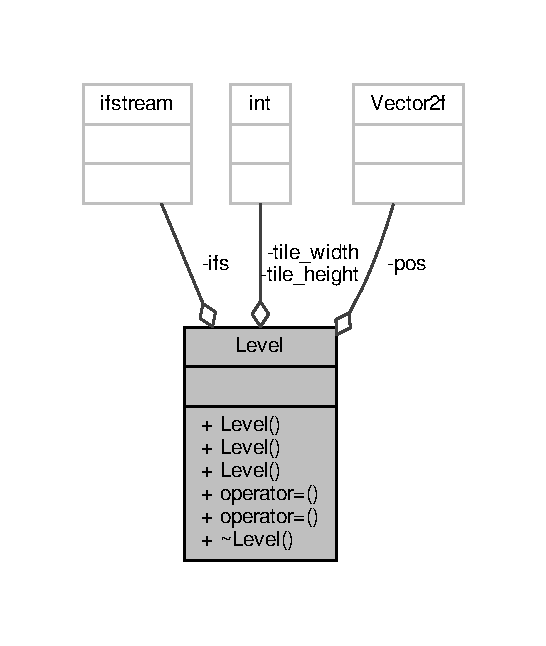
\includegraphics[width=262pt]{classLevel__coll__graph}
\end{center}
\end{figure}
\subsection*{Public Member Functions}
\begin{DoxyCompactItemize}
\item 
\hyperlink{classLevel_a9c1885f00f43c9b88eed9d103dd87408}{Level} (std\+::string, int, int, \hyperlink{classWorld}{World} \&, int)
\item 
\hyperlink{classLevel_acaeb0c9b638c74795b6608635af5b338}{Level} (\hyperlink{classLevel}{Level} const \&other)=delete
\begin{DoxyCompactList}\small\item\em Copy konstruktor. \end{DoxyCompactList}\item 
\hyperlink{classLevel_a5535d562f2ec6c4e08b65fa216933127}{Level} (\hyperlink{classLevel}{Level} \&\&other)=delete
\begin{DoxyCompactList}\small\item\em Move konstruktor. \end{DoxyCompactList}\item 
\hyperlink{classLevel}{Level} \& \hyperlink{classLevel_a182dd33b1b7821359aee3600351d4778}{operator=} (\hyperlink{classLevel}{Level} const \&rhs)\&=delete
\begin{DoxyCompactList}\small\item\em Copy operator. \end{DoxyCompactList}\item 
\hyperlink{classLevel}{Level} \& \hyperlink{classLevel_a89cfea51f0b0f91bbd1e33839c9dc211}{operator=} (\hyperlink{classLevel}{Level} \&\&rhs)=delete
\begin{DoxyCompactList}\small\item\em Move operator. \end{DoxyCompactList}\item 
\hyperlink{classLevel_ac6cdb61bec67832b3db9e5874b479c0d}{$\sim$\+Level} ()=default
\begin{DoxyCompactList}\small\item\em Default destruktor. \end{DoxyCompactList}\end{DoxyCompactItemize}
\subsection*{Private Attributes}
\begin{DoxyCompactItemize}
\item 
std\+::ifstream \hyperlink{classLevel_aa1a8e3b1ba0606c3c461624b5af8172c}{ifs}
\begin{DoxyCompactList}\small\item\em En input file stream för att kunna läsa från en fil. \end{DoxyCompactList}\item 
int \hyperlink{classLevel_ac846cb2f8b1bd0f92a60a484ce1e50ef}{tile\+\_\+width}
\begin{DoxyCompactList}\small\item\em Variabel för att spara undan bredd. \end{DoxyCompactList}\item 
int \hyperlink{classLevel_a75ae0539332f57c52edac380fa0fc0c3}{tile\+\_\+height}
\begin{DoxyCompactList}\small\item\em Variabel för att spara undan höjd. \end{DoxyCompactList}\item 
sf\+::\+Vector2f \hyperlink{classLevel_a23a51431287bd8692a998de1b1fdf884}{pos}
\begin{DoxyCompactList}\small\item\em Vilken position vi just nu arbetar på. \end{DoxyCompactList}\end{DoxyCompactItemize}


\subsection{Detailed Description}
\hyperlink{classLevel}{Level} läser in från .lvl filer och skapar entiteter till \hyperlink{classWorld}{World}. 

\hyperlink{classLevel}{Level} läser in en fil som har skapats specifikt för det här projektet. Den innehåller information om hur spelvärlden ska se ut, var fiender ska finnas och var spelaren ska starta. Den skapar sedan dessa entititer och lägger till dem i \hyperlink{classWorld_a74d706a3a47afe52b70f5e2dd3bf612b}{World.\+entities}. 

\subsection{Constructor \& Destructor Documentation}
\hypertarget{classLevel_a9c1885f00f43c9b88eed9d103dd87408}{\index{Level@{Level}!Level@{Level}}
\index{Level@{Level}!Level@{Level}}
\subsubsection[{Level}]{\setlength{\rightskip}{0pt plus 5cm}Level\+::\+Level (
\begin{DoxyParamCaption}
\item[{std\+::string}]{filename, }
\item[{int}]{w, }
\item[{int}]{h, }
\item[{{\bf World} \&}]{world, }
\item[{int}]{player\+\_\+amount}
\end{DoxyParamCaption}
)}}\label{classLevel_a9c1885f00f43c9b88eed9d103dd87408}
Allting händer här i konstruktorn. Konstruktorn tar in en sökväg, bredd och höjd på varje tile, en värld som den ska skriva till och antalet spelare i världen. \hypertarget{classLevel_acaeb0c9b638c74795b6608635af5b338}{\index{Level@{Level}!Level@{Level}}
\index{Level@{Level}!Level@{Level}}
\subsubsection[{Level}]{\setlength{\rightskip}{0pt plus 5cm}Level\+::\+Level (
\begin{DoxyParamCaption}
\item[{{\bf Level} const \&}]{other}
\end{DoxyParamCaption}
)\hspace{0.3cm}{\ttfamily [delete]}}}\label{classLevel_acaeb0c9b638c74795b6608635af5b338}


Copy konstruktor. 

\hypertarget{classLevel_a5535d562f2ec6c4e08b65fa216933127}{\index{Level@{Level}!Level@{Level}}
\index{Level@{Level}!Level@{Level}}
\subsubsection[{Level}]{\setlength{\rightskip}{0pt plus 5cm}Level\+::\+Level (
\begin{DoxyParamCaption}
\item[{{\bf Level} \&\&}]{other}
\end{DoxyParamCaption}
)\hspace{0.3cm}{\ttfamily [delete]}}}\label{classLevel_a5535d562f2ec6c4e08b65fa216933127}


Move konstruktor. 

\hypertarget{classLevel_ac6cdb61bec67832b3db9e5874b479c0d}{\index{Level@{Level}!````~Level@{$\sim$\+Level}}
\index{````~Level@{$\sim$\+Level}!Level@{Level}}
\subsubsection[{$\sim$\+Level}]{\setlength{\rightskip}{0pt plus 5cm}Level\+::$\sim$\+Level (
\begin{DoxyParamCaption}
{}
\end{DoxyParamCaption}
)\hspace{0.3cm}{\ttfamily [default]}}}\label{classLevel_ac6cdb61bec67832b3db9e5874b479c0d}


Default destruktor. 



\subsection{Member Function Documentation}
\hypertarget{classLevel_a182dd33b1b7821359aee3600351d4778}{\index{Level@{Level}!operator=@{operator=}}
\index{operator=@{operator=}!Level@{Level}}
\subsubsection[{operator=}]{\setlength{\rightskip}{0pt plus 5cm}{\bf Level}\& Level\+::operator= (
\begin{DoxyParamCaption}
\item[{{\bf Level} const \&}]{rhs}
\end{DoxyParamCaption}
)\hspace{0.3cm}{\ttfamily [delete]}}}\label{classLevel_a182dd33b1b7821359aee3600351d4778}


Copy operator. 

\hypertarget{classLevel_a89cfea51f0b0f91bbd1e33839c9dc211}{\index{Level@{Level}!operator=@{operator=}}
\index{operator=@{operator=}!Level@{Level}}
\subsubsection[{operator=}]{\setlength{\rightskip}{0pt plus 5cm}{\bf Level}\& Level\+::operator= (
\begin{DoxyParamCaption}
\item[{{\bf Level} \&\&}]{rhs}
\end{DoxyParamCaption}
)\hspace{0.3cm}{\ttfamily [delete]}}}\label{classLevel_a89cfea51f0b0f91bbd1e33839c9dc211}


Move operator. 



\subsection{Member Data Documentation}
\hypertarget{classLevel_aa1a8e3b1ba0606c3c461624b5af8172c}{\index{Level@{Level}!ifs@{ifs}}
\index{ifs@{ifs}!Level@{Level}}
\subsubsection[{ifs}]{\setlength{\rightskip}{0pt plus 5cm}std\+::ifstream Level\+::ifs\hspace{0.3cm}{\ttfamily [private]}}}\label{classLevel_aa1a8e3b1ba0606c3c461624b5af8172c}


En input file stream för att kunna läsa från en fil. 

\hypertarget{classLevel_a23a51431287bd8692a998de1b1fdf884}{\index{Level@{Level}!pos@{pos}}
\index{pos@{pos}!Level@{Level}}
\subsubsection[{pos}]{\setlength{\rightskip}{0pt plus 5cm}sf\+::\+Vector2f Level\+::pos\hspace{0.3cm}{\ttfamily [private]}}}\label{classLevel_a23a51431287bd8692a998de1b1fdf884}


Vilken position vi just nu arbetar på. 

\hypertarget{classLevel_a75ae0539332f57c52edac380fa0fc0c3}{\index{Level@{Level}!tile\+\_\+height@{tile\+\_\+height}}
\index{tile\+\_\+height@{tile\+\_\+height}!Level@{Level}}
\subsubsection[{tile\+\_\+height}]{\setlength{\rightskip}{0pt plus 5cm}int Level\+::tile\+\_\+height\hspace{0.3cm}{\ttfamily [private]}}}\label{classLevel_a75ae0539332f57c52edac380fa0fc0c3}


Variabel för att spara undan höjd. 

\hypertarget{classLevel_ac846cb2f8b1bd0f92a60a484ce1e50ef}{\index{Level@{Level}!tile\+\_\+width@{tile\+\_\+width}}
\index{tile\+\_\+width@{tile\+\_\+width}!Level@{Level}}
\subsubsection[{tile\+\_\+width}]{\setlength{\rightskip}{0pt plus 5cm}int Level\+::tile\+\_\+width\hspace{0.3cm}{\ttfamily [private]}}}\label{classLevel_ac846cb2f8b1bd0f92a60a484ce1e50ef}


Variabel för att spara undan bredd. 



The documentation for this class was generated from the following files\+:\begin{DoxyCompactItemize}
\item 
source/objects/headers/Level.\+h\item 
source/objects/imps/Level.\+cpp\end{DoxyCompactItemize}

\hypertarget{classMenu}{\section{Menu Class Reference}
\label{classMenu}\index{Menu@{Menu}}
}


\hyperlink{classMenu}{Menu} har hand om menyer innan man börjar spela spelet.  




{\ttfamily \#include $<$Menu.\+h$>$}



Collaboration diagram for Menu\+:\nopagebreak
\begin{figure}[H]
\begin{center}
\leavevmode
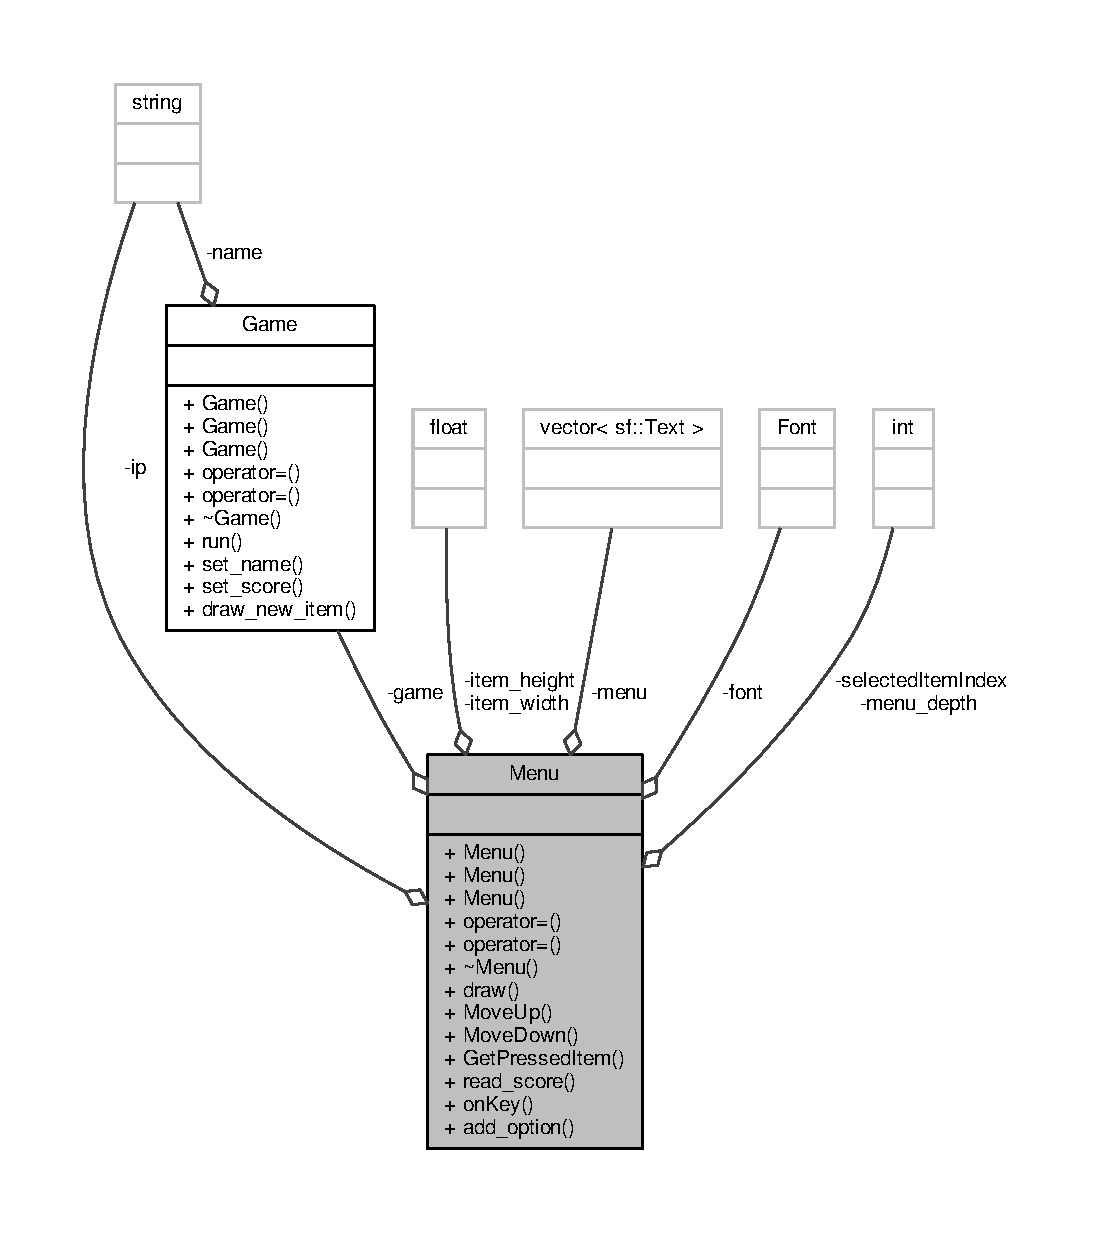
\includegraphics[width=350pt]{classMenu__coll__graph}
\end{center}
\end{figure}
\subsection*{Public Member Functions}
\begin{DoxyCompactItemize}
\item 
\hyperlink{classMenu_a8caa6100506d4b8e0d782e550dbc470e}{Menu} (float width, float height)
\item 
\hyperlink{classMenu_a3c4832a05323c234e6bb9b949b768bcd}{Menu} (\hyperlink{classMenu}{Menu} const \&other)=delete
\begin{DoxyCompactList}\small\item\em Copy konstruktor. \end{DoxyCompactList}\item 
\hyperlink{classMenu_a31b3412d1fa95e0acb0dd931add9df44}{Menu} (\hyperlink{classMenu}{Menu} \&\&other)=delete
\begin{DoxyCompactList}\small\item\em Move konstruktor. \end{DoxyCompactList}\item 
\hyperlink{classMenu}{Menu} \& \hyperlink{classMenu_ac388d81e62249a18c2ba186a25c5f5b0}{operator=} (\hyperlink{classMenu}{Menu} const \&rhs)\&=delete
\begin{DoxyCompactList}\small\item\em Copy operator. \end{DoxyCompactList}\item 
\hyperlink{classMenu}{Menu} \& \hyperlink{classMenu_aa14291c8988294534bae31188a0aa70b}{operator=} (\hyperlink{classMenu}{Menu} \&\&rhs)=delete
\begin{DoxyCompactList}\small\item\em Move operator. \end{DoxyCompactList}\item 
\hyperlink{classMenu_aec66e8695cecd5e88732d20ffd027921}{$\sim$\+Menu} ()=default
\begin{DoxyCompactList}\small\item\em Default Destruktor. \end{DoxyCompactList}\item 
void \hyperlink{classMenu_a1443dcfd1c1c9844c40658d752c1fbab}{draw} (sf\+::\+Render\+Window \&window)
\begin{DoxyCompactList}\small\item\em Ritar ut alla meny objekt. \end{DoxyCompactList}\item 
void \hyperlink{classMenu_acfb038bbd1050d6c55c86eec1f35dbdb}{Move\+Up} ()
\item 
void \hyperlink{classMenu_a804da9a381bb6c633d5d2bc4f839ec62}{Move\+Down} ()
\item 
int \hyperlink{classMenu_a81b2029bf7783f38be26000969e99e30}{Get\+Pressed\+Item} ()
\begin{DoxyCompactList}\small\item\em Tar fram vilken del av menyn som tryckts på. \end{DoxyCompactList}\item 
void \hyperlink{classMenu_acd0c45fbf5c84d5de059c8b1b2d33bfa}{read\+\_\+score} (sf\+::\+Render\+Window \&window)
\item 
void \hyperlink{classMenu_a6cfb83fb8f947ab6e1b4c101a5326814}{on\+Key} (sf\+::\+Keyboard\+::\+Key const \&key, sf\+::\+Render\+Window \&)
\item 
void \hyperlink{classMenu_a5b2f54c794ca701d433caf755b83765e}{add\+\_\+option} (std\+::string, float)
\end{DoxyCompactItemize}
\subsection*{Private Attributes}
\begin{DoxyCompactItemize}
\item 
float \hyperlink{classMenu_a8dd7434d066c508cb0bc6b7a16d3896c}{item\+\_\+width}
\begin{DoxyCompactList}\small\item\em Variabel för fönstrets bredd. \end{DoxyCompactList}\item 
float \hyperlink{classMenu_a715ee3491fe1a3f34061a5a17ef4871e}{item\+\_\+height}
\begin{DoxyCompactList}\small\item\em Variabel för fönstrets höjd. \end{DoxyCompactList}\item 
int \hyperlink{classMenu_a0b9b3614aefa98bd42a9c54984784f15}{menu\+\_\+depth}
\item 
int \hyperlink{classMenu_a464ef16fd28c0df35ee1d9f78c0ef895}{selected\+Item\+Index}
\item 
sf\+::\+Font \hyperlink{classMenu_a9446727ebf60c6063218b5d4bcae170a}{font}
\item 
std\+::vector$<$ sf\+::\+Text $>$ \hyperlink{classMenu_ae0638a87425d6d01ce8b5c3508e4a642}{menu}
\item 
\hyperlink{classGame}{Game} \hyperlink{classMenu_a600e0c5a79a2200f64d7c3d5626c026d}{game} \{\}
\begin{DoxyCompactList}\small\item\em En instans av \hyperlink{classGame}{Game}. Sparas så att den inte går utanför scope. \end{DoxyCompactList}\item 
std\+::string \hyperlink{classMenu_ae225c68be6780e064e5f1e6f57d68d5e}{ip}
\begin{DoxyCompactList}\small\item\em Variabel som sparar din ip. Används för. \end{DoxyCompactList}\end{DoxyCompactItemize}


\subsection{Detailed Description}
\hyperlink{classMenu}{Menu} har hand om menyer innan man börjar spela spelet. 

\hyperlink{classMenu}{Menu} skapar, ritar ut och hanterar input i de menyer spelet har innan spelet startar. Det använder sig av std\+::string och sf\+::\+Text för att skapa listor av val som användaren sedan kan välja med hjälp av piltangenterna och enter. 

\subsection{Constructor \& Destructor Documentation}
\hypertarget{classMenu_a8caa6100506d4b8e0d782e550dbc470e}{\index{Menu@{Menu}!Menu@{Menu}}
\index{Menu@{Menu}!Menu@{Menu}}
\subsubsection[{Menu}]{\setlength{\rightskip}{0pt plus 5cm}Menu\+::\+Menu (
\begin{DoxyParamCaption}
\item[{float}]{width, }
\item[{float}]{height}
\end{DoxyParamCaption}
)}}\label{classMenu_a8caa6100506d4b8e0d782e550dbc470e}
Konstruktor som tar in 2 floats. 1 för bredd och 1 för höjd på fönstret. \hypertarget{classMenu_a3c4832a05323c234e6bb9b949b768bcd}{\index{Menu@{Menu}!Menu@{Menu}}
\index{Menu@{Menu}!Menu@{Menu}}
\subsubsection[{Menu}]{\setlength{\rightskip}{0pt plus 5cm}Menu\+::\+Menu (
\begin{DoxyParamCaption}
\item[{{\bf Menu} const \&}]{other}
\end{DoxyParamCaption}
)\hspace{0.3cm}{\ttfamily [delete]}}}\label{classMenu_a3c4832a05323c234e6bb9b949b768bcd}


Copy konstruktor. 

\hypertarget{classMenu_a31b3412d1fa95e0acb0dd931add9df44}{\index{Menu@{Menu}!Menu@{Menu}}
\index{Menu@{Menu}!Menu@{Menu}}
\subsubsection[{Menu}]{\setlength{\rightskip}{0pt plus 5cm}Menu\+::\+Menu (
\begin{DoxyParamCaption}
\item[{{\bf Menu} \&\&}]{other}
\end{DoxyParamCaption}
)\hspace{0.3cm}{\ttfamily [delete]}}}\label{classMenu_a31b3412d1fa95e0acb0dd931add9df44}


Move konstruktor. 

\hypertarget{classMenu_aec66e8695cecd5e88732d20ffd027921}{\index{Menu@{Menu}!````~Menu@{$\sim$\+Menu}}
\index{````~Menu@{$\sim$\+Menu}!Menu@{Menu}}
\subsubsection[{$\sim$\+Menu}]{\setlength{\rightskip}{0pt plus 5cm}Menu\+::$\sim$\+Menu (
\begin{DoxyParamCaption}
{}
\end{DoxyParamCaption}
)\hspace{0.3cm}{\ttfamily [default]}}}\label{classMenu_aec66e8695cecd5e88732d20ffd027921}


Default Destruktor. 



\subsection{Member Function Documentation}
\hypertarget{classMenu_a5b2f54c794ca701d433caf755b83765e}{\index{Menu@{Menu}!add\+\_\+option@{add\+\_\+option}}
\index{add\+\_\+option@{add\+\_\+option}!Menu@{Menu}}
\subsubsection[{add\+\_\+option}]{\setlength{\rightskip}{0pt plus 5cm}void Menu\+::add\+\_\+option (
\begin{DoxyParamCaption}
\item[{std\+::string}]{s, }
\item[{float}]{f}
\end{DoxyParamCaption}
)}}\label{classMenu_a5b2f54c794ca701d433caf755b83765e}
Lägger till ett nytt meny val. Tar in en sträng och formaterar den till en sf\+::\+Text. \hypertarget{classMenu_a1443dcfd1c1c9844c40658d752c1fbab}{\index{Menu@{Menu}!draw@{draw}}
\index{draw@{draw}!Menu@{Menu}}
\subsubsection[{draw}]{\setlength{\rightskip}{0pt plus 5cm}void Menu\+::draw (
\begin{DoxyParamCaption}
\item[{sf\+::\+Render\+Window \&}]{window}
\end{DoxyParamCaption}
)}}\label{classMenu_a1443dcfd1c1c9844c40658d752c1fbab}


Ritar ut alla meny objekt. 

\hypertarget{classMenu_a81b2029bf7783f38be26000969e99e30}{\index{Menu@{Menu}!Get\+Pressed\+Item@{Get\+Pressed\+Item}}
\index{Get\+Pressed\+Item@{Get\+Pressed\+Item}!Menu@{Menu}}
\subsubsection[{Get\+Pressed\+Item}]{\setlength{\rightskip}{0pt plus 5cm}int Menu\+::\+Get\+Pressed\+Item (
\begin{DoxyParamCaption}
{}
\end{DoxyParamCaption}
)\hspace{0.3cm}{\ttfamily [inline]}}}\label{classMenu_a81b2029bf7783f38be26000969e99e30}


Tar fram vilken del av menyn som tryckts på. 

\hypertarget{classMenu_a804da9a381bb6c633d5d2bc4f839ec62}{\index{Menu@{Menu}!Move\+Down@{Move\+Down}}
\index{Move\+Down@{Move\+Down}!Menu@{Menu}}
\subsubsection[{Move\+Down}]{\setlength{\rightskip}{0pt plus 5cm}void Menu\+::\+Move\+Down (
\begin{DoxyParamCaption}
{}
\end{DoxyParamCaption}
)}}\label{classMenu_a804da9a381bb6c633d5d2bc4f839ec62}
Flyttar ner ett meny val men flyttar också till första om selected index är det sista. \hypertarget{classMenu_acfb038bbd1050d6c55c86eec1f35dbdb}{\index{Menu@{Menu}!Move\+Up@{Move\+Up}}
\index{Move\+Up@{Move\+Up}!Menu@{Menu}}
\subsubsection[{Move\+Up}]{\setlength{\rightskip}{0pt plus 5cm}void Menu\+::\+Move\+Up (
\begin{DoxyParamCaption}
{}
\end{DoxyParamCaption}
)}}\label{classMenu_acfb038bbd1050d6c55c86eec1f35dbdb}
Flyttar upp ett meny val men flyttar också till sista om selected index är det första. \hypertarget{classMenu_a6cfb83fb8f947ab6e1b4c101a5326814}{\index{Menu@{Menu}!on\+Key@{on\+Key}}
\index{on\+Key@{on\+Key}!Menu@{Menu}}
\subsubsection[{on\+Key}]{\setlength{\rightskip}{0pt plus 5cm}void Menu\+::on\+Key (
\begin{DoxyParamCaption}
\item[{sf\+::\+Keyboard\+::\+Key const \&}]{key, }
\item[{sf\+::\+Render\+Window \&}]{w}
\end{DoxyParamCaption}
)}}\label{classMenu_a6cfb83fb8f947ab6e1b4c101a5326814}
Tar hand om knapptryckningar i menyn. Om man kommer till slutet av menyn och fortsätter så börjar man om i början av menyn. \hypertarget{classMenu_ac388d81e62249a18c2ba186a25c5f5b0}{\index{Menu@{Menu}!operator=@{operator=}}
\index{operator=@{operator=}!Menu@{Menu}}
\subsubsection[{operator=}]{\setlength{\rightskip}{0pt plus 5cm}{\bf Menu}\& Menu\+::operator= (
\begin{DoxyParamCaption}
\item[{{\bf Menu} const \&}]{rhs}
\end{DoxyParamCaption}
)\hspace{0.3cm}{\ttfamily [delete]}}}\label{classMenu_ac388d81e62249a18c2ba186a25c5f5b0}


Copy operator. 

\hypertarget{classMenu_aa14291c8988294534bae31188a0aa70b}{\index{Menu@{Menu}!operator=@{operator=}}
\index{operator=@{operator=}!Menu@{Menu}}
\subsubsection[{operator=}]{\setlength{\rightskip}{0pt plus 5cm}{\bf Menu}\& Menu\+::operator= (
\begin{DoxyParamCaption}
\item[{{\bf Menu} \&\&}]{rhs}
\end{DoxyParamCaption}
)\hspace{0.3cm}{\ttfamily [delete]}}}\label{classMenu_aa14291c8988294534bae31188a0aa70b}


Move operator. 

\hypertarget{classMenu_acd0c45fbf5c84d5de059c8b1b2d33bfa}{\index{Menu@{Menu}!read\+\_\+score@{read\+\_\+score}}
\index{read\+\_\+score@{read\+\_\+score}!Menu@{Menu}}
\subsubsection[{read\+\_\+score}]{\setlength{\rightskip}{0pt plus 5cm}void Menu\+::read\+\_\+score (
\begin{DoxyParamCaption}
\item[{sf\+::\+Render\+Window \&}]{window}
\end{DoxyParamCaption}
)}}\label{classMenu_acd0c45fbf5c84d5de059c8b1b2d33bfa}
Läser in high score från score filen. Formaterar sedan dessa som meny val och låter menyn skriva ut dem. 

\subsection{Member Data Documentation}
\hypertarget{classMenu_a9446727ebf60c6063218b5d4bcae170a}{\index{Menu@{Menu}!font@{font}}
\index{font@{font}!Menu@{Menu}}
\subsubsection[{font}]{\setlength{\rightskip}{0pt plus 5cm}sf\+::\+Font Menu\+::font\hspace{0.3cm}{\ttfamily [private]}}}\label{classMenu_a9446727ebf60c6063218b5d4bcae170a}
Variabel för att spara vilken font menyn ska ha. Om man inte sparar den så försvinner den när den går ur scope. \hypertarget{classMenu_a600e0c5a79a2200f64d7c3d5626c026d}{\index{Menu@{Menu}!game@{game}}
\index{game@{game}!Menu@{Menu}}
\subsubsection[{game}]{\setlength{\rightskip}{0pt plus 5cm}{\bf Game} Menu\+::game \{\}\hspace{0.3cm}{\ttfamily [private]}}}\label{classMenu_a600e0c5a79a2200f64d7c3d5626c026d}


En instans av \hyperlink{classGame}{Game}. Sparas så att den inte går utanför scope. 

\hypertarget{classMenu_ae225c68be6780e064e5f1e6f57d68d5e}{\index{Menu@{Menu}!ip@{ip}}
\index{ip@{ip}!Menu@{Menu}}
\subsubsection[{ip}]{\setlength{\rightskip}{0pt plus 5cm}std\+::string Menu\+::ip\hspace{0.3cm}{\ttfamily [private]}}}\label{classMenu_ae225c68be6780e064e5f1e6f57d68d5e}


Variabel som sparar din ip. Används för. 

\hypertarget{classMenu_a715ee3491fe1a3f34061a5a17ef4871e}{\index{Menu@{Menu}!item\+\_\+height@{item\+\_\+height}}
\index{item\+\_\+height@{item\+\_\+height}!Menu@{Menu}}
\subsubsection[{item\+\_\+height}]{\setlength{\rightskip}{0pt plus 5cm}float Menu\+::item\+\_\+height\hspace{0.3cm}{\ttfamily [private]}}}\label{classMenu_a715ee3491fe1a3f34061a5a17ef4871e}


Variabel för fönstrets höjd. 

\hypertarget{classMenu_a8dd7434d066c508cb0bc6b7a16d3896c}{\index{Menu@{Menu}!item\+\_\+width@{item\+\_\+width}}
\index{item\+\_\+width@{item\+\_\+width}!Menu@{Menu}}
\subsubsection[{item\+\_\+width}]{\setlength{\rightskip}{0pt plus 5cm}float Menu\+::item\+\_\+width\hspace{0.3cm}{\ttfamily [private]}}}\label{classMenu_a8dd7434d066c508cb0bc6b7a16d3896c}


Variabel för fönstrets bredd. 

\hypertarget{classMenu_ae0638a87425d6d01ce8b5c3508e4a642}{\index{Menu@{Menu}!menu@{menu}}
\index{menu@{menu}!Menu@{Menu}}
\subsubsection[{menu}]{\setlength{\rightskip}{0pt plus 5cm}std\+::vector$<$sf\+::\+Text$>$ Menu\+::menu\hspace{0.3cm}{\ttfamily [private]}}}\label{classMenu_ae0638a87425d6d01ce8b5c3508e4a642}
En std\+::vector som innehåller sf\+::\+Text objekt som representerar en del i menyn. \hypertarget{classMenu_a0b9b3614aefa98bd42a9c54984784f15}{\index{Menu@{Menu}!menu\+\_\+depth@{menu\+\_\+depth}}
\index{menu\+\_\+depth@{menu\+\_\+depth}!Menu@{Menu}}
\subsubsection[{menu\+\_\+depth}]{\setlength{\rightskip}{0pt plus 5cm}int Menu\+::menu\+\_\+depth\hspace{0.3cm}{\ttfamily [private]}}}\label{classMenu_a0b9b3614aefa98bd42a9c54984784f15}
Variabel för meny djupet. Detta för att kunna ha mer än 1 meny med flera olika beteenden. \hypertarget{classMenu_a464ef16fd28c0df35ee1d9f78c0ef895}{\index{Menu@{Menu}!selected\+Item\+Index@{selected\+Item\+Index}}
\index{selected\+Item\+Index@{selected\+Item\+Index}!Menu@{Menu}}
\subsubsection[{selected\+Item\+Index}]{\setlength{\rightskip}{0pt plus 5cm}int Menu\+::selected\+Item\+Index\hspace{0.3cm}{\ttfamily [private]}}}\label{classMenu_a464ef16fd28c0df35ee1d9f78c0ef895}
Variabel för vilken del av menyn som är vald. Den highlightas och är också den som beteendet baseras på. 

The documentation for this class was generated from the following files\+:\begin{DoxyCompactItemize}
\item 
source/objects/headers/Menu.\+h\item 
source/objects/imps/Menu.\+cpp\end{DoxyCompactItemize}

\hypertarget{classPlatform}{\section{Platform Class Reference}
\label{classPlatform}\index{Platform@{Platform}}
}


\hyperlink{classPlatform}{Platform} ärver från \hyperlink{classEntity}{Entity} och innehåller all information för en entitet av platformstyp.  




{\ttfamily \#include $<$Platform.\+h$>$}



Inheritance diagram for Platform\+:\nopagebreak
\begin{figure}[H]
\begin{center}
\leavevmode
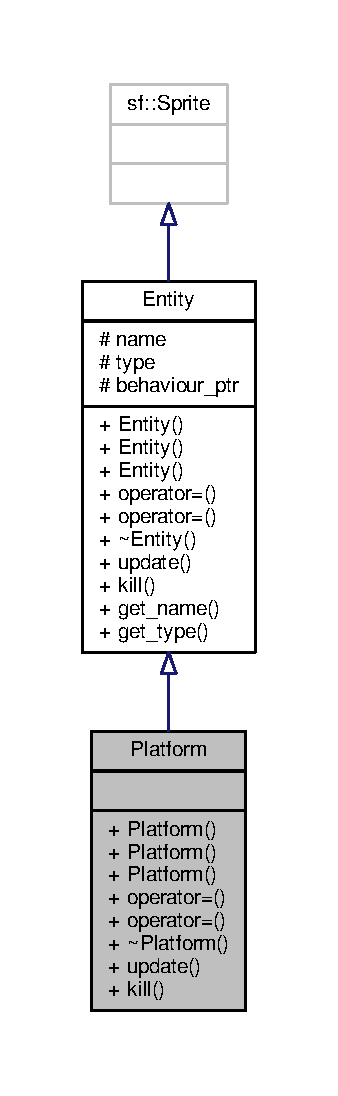
\includegraphics[width=162pt]{classPlatform__inherit__graph}
\end{center}
\end{figure}


Collaboration diagram for Platform\+:\nopagebreak
\begin{figure}[H]
\begin{center}
\leavevmode
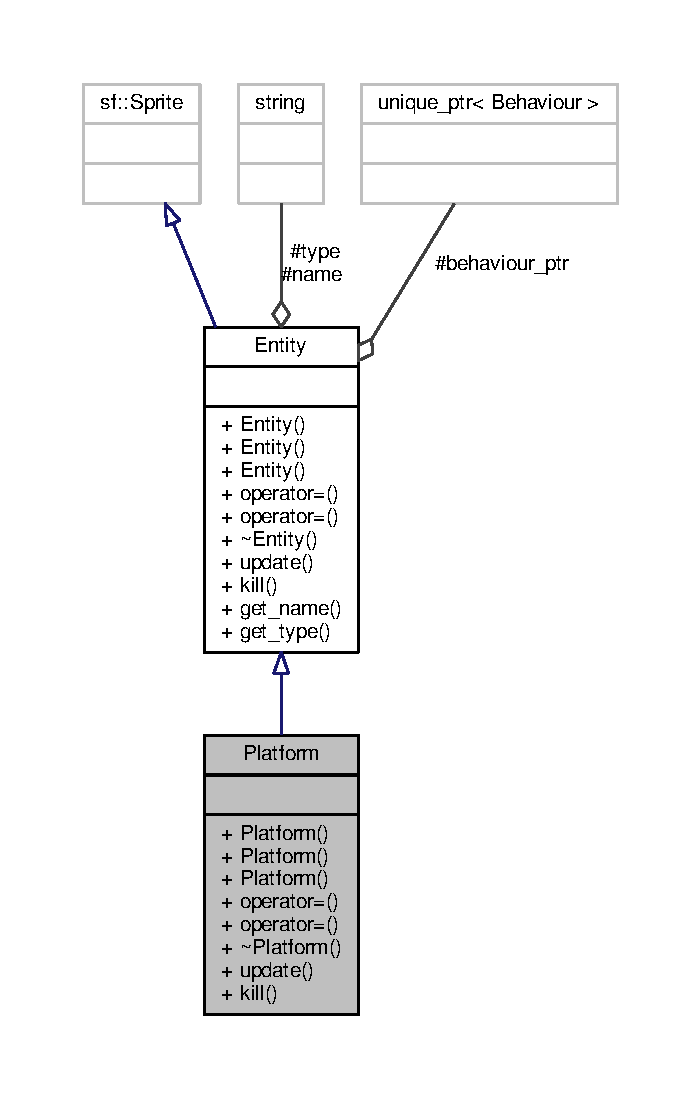
\includegraphics[width=336pt]{classPlatform__coll__graph}
\end{center}
\end{figure}
\subsection*{Public Member Functions}
\begin{DoxyCompactItemize}
\item 
\hyperlink{classPlatform_a87ebc22e56d673fede211c6824f015f6}{Platform} (std\+::string, std\+::string, \hyperlink{classBehaviour}{Behaviour} $\ast$, sf\+::\+Vector2f, sf\+::\+Texture const \&, sf\+::\+Int\+Rect)
\item 
\hyperlink{classPlatform_a187acbd90dbed1c028d640d19d69fedd}{Platform} (\hyperlink{classPlatform}{Platform} const \&other)=delete
\begin{DoxyCompactList}\small\item\em Copy konstruktor. \end{DoxyCompactList}\item 
\hyperlink{classPlatform_a62adfd45ef427798c713064cd54b926b}{Platform} (\hyperlink{classPlatform}{Platform} \&\&other)=delete
\begin{DoxyCompactList}\small\item\em Move konstruktor. \end{DoxyCompactList}\item 
\hyperlink{classPlatform}{Platform} \& \hyperlink{classPlatform_a80d5d52e630409f5ae9a1cd98720faf2}{operator=} (\hyperlink{classPlatform}{Platform} const \&rhs)\&=delete
\begin{DoxyCompactList}\small\item\em Copy operator. \end{DoxyCompactList}\item 
\hyperlink{classPlatform}{Platform} \& \hyperlink{classPlatform_af57a590654b1c1c2432e79237de854f9}{operator=} (\hyperlink{classPlatform}{Platform} \&\&rhs)=delete
\begin{DoxyCompactList}\small\item\em Move operator. \end{DoxyCompactList}\item 
\hyperlink{classPlatform_ab1def8463428a10d2fe399fd695118f9}{$\sim$\+Platform} ()=default
\begin{DoxyCompactList}\small\item\em Default Destruktor. \end{DoxyCompactList}\item 
void \hyperlink{classPlatform_ad756e0494312cdd8956af8bee6afbb0f}{update} (\hyperlink{classWorld}{World} \&, sf\+::\+Time const \&) override
\item 
void \hyperlink{classPlatform_a6dd2fe10f6de044db339c5050bdb7ef0}{kill} (\hyperlink{classWorld}{World} \&w) override
\begin{DoxyCompactList}\small\item\em Om det här objektet har dödats så kommer kill att göra det genom att informera \hyperlink{classWorld}{World} om det. \end{DoxyCompactList}\item 
std\+::string \hyperlink{classEntity_a75c7e4aad3df2e053ee5b43169509534}{get\+\_\+name} () const 
\begin{DoxyCompactList}\small\item\em Returnerar namnet på entititen. \end{DoxyCompactList}\item 
std\+::string \hyperlink{classEntity_a0e9ef479c1147e21e5bcb338cb858df2}{get\+\_\+type} () const 
\begin{DoxyCompactList}\small\item\em Returnerar typen på entititen. \end{DoxyCompactList}\end{DoxyCompactItemize}
\subsection*{Protected Attributes}
\begin{DoxyCompactItemize}
\item 
std\+::string \hyperlink{classEntity_a931b21fbdebb1a5963b4bcab5df128f5}{name}
\begin{DoxyCompactList}\small\item\em Namn. \end{DoxyCompactList}\item 
std\+::string \hyperlink{classEntity_a298a9ebf2474bb00874b5ff6a0d637ef}{type}
\begin{DoxyCompactList}\small\item\em Typ. \end{DoxyCompactList}\item 
std\+::unique\+\_\+ptr$<$ \hyperlink{classBehaviour}{Behaviour} $>$ \hyperlink{classEntity_adb6e36848db24e6d48e6d295e19d3972}{behaviour\+\_\+ptr}
\begin{DoxyCompactList}\small\item\em Unik smart-\/pekare till ett objekt av \hyperlink{classBehaviour}{Behaviour} klassen. \end{DoxyCompactList}\end{DoxyCompactItemize}


\subsection{Detailed Description}
\hyperlink{classPlatform}{Platform} ärver från \hyperlink{classEntity}{Entity} och innehåller all information för en entitet av platformstyp. 

\hyperlink{classPlatform}{Platform} ärver från den abstrakta grundklassen \hyperlink{classEntity}{Entity} och innehåller information om platformar i spelet. 

\subsection{Constructor \& Destructor Documentation}
\hypertarget{classPlatform_a87ebc22e56d673fede211c6824f015f6}{\index{Platform@{Platform}!Platform@{Platform}}
\index{Platform@{Platform}!Platform@{Platform}}
\subsubsection[{Platform}]{\setlength{\rightskip}{0pt plus 5cm}Platform\+::\+Platform (
\begin{DoxyParamCaption}
\item[{std\+::string}]{n, }
\item[{std\+::string}]{t, }
\item[{{\bf Behaviour} $\ast$}]{b, }
\item[{sf\+::\+Vector2f}]{pos, }
\item[{sf\+::\+Texture const \&}]{texture, }
\item[{sf\+::\+Int\+Rect}]{size}
\end{DoxyParamCaption}
)}}\label{classPlatform_a87ebc22e56d673fede211c6824f015f6}
Platforms konstruktor Tar in ett namn, en typ, en \hyperlink{classBehaviour}{Behaviour} pekare, en sf\+::\+Vector2f för position, ett textur referens och vilken kvadrat som ska ritas ut. \hypertarget{classPlatform_a187acbd90dbed1c028d640d19d69fedd}{\index{Platform@{Platform}!Platform@{Platform}}
\index{Platform@{Platform}!Platform@{Platform}}
\subsubsection[{Platform}]{\setlength{\rightskip}{0pt plus 5cm}Platform\+::\+Platform (
\begin{DoxyParamCaption}
\item[{{\bf Platform} const \&}]{other}
\end{DoxyParamCaption}
)\hspace{0.3cm}{\ttfamily [delete]}}}\label{classPlatform_a187acbd90dbed1c028d640d19d69fedd}


Copy konstruktor. 

\hypertarget{classPlatform_a62adfd45ef427798c713064cd54b926b}{\index{Platform@{Platform}!Platform@{Platform}}
\index{Platform@{Platform}!Platform@{Platform}}
\subsubsection[{Platform}]{\setlength{\rightskip}{0pt plus 5cm}Platform\+::\+Platform (
\begin{DoxyParamCaption}
\item[{{\bf Platform} \&\&}]{other}
\end{DoxyParamCaption}
)\hspace{0.3cm}{\ttfamily [delete]}}}\label{classPlatform_a62adfd45ef427798c713064cd54b926b}


Move konstruktor. 

\hypertarget{classPlatform_ab1def8463428a10d2fe399fd695118f9}{\index{Platform@{Platform}!````~Platform@{$\sim$\+Platform}}
\index{````~Platform@{$\sim$\+Platform}!Platform@{Platform}}
\subsubsection[{$\sim$\+Platform}]{\setlength{\rightskip}{0pt plus 5cm}Platform\+::$\sim$\+Platform (
\begin{DoxyParamCaption}
{}
\end{DoxyParamCaption}
)\hspace{0.3cm}{\ttfamily [default]}}}\label{classPlatform_ab1def8463428a10d2fe399fd695118f9}


Default Destruktor. 



\subsection{Member Function Documentation}
\hypertarget{classEntity_a75c7e4aad3df2e053ee5b43169509534}{\index{Platform@{Platform}!get\+\_\+name@{get\+\_\+name}}
\index{get\+\_\+name@{get\+\_\+name}!Platform@{Platform}}
\subsubsection[{get\+\_\+name}]{\setlength{\rightskip}{0pt plus 5cm}std\+::string Entity\+::get\+\_\+name (
\begin{DoxyParamCaption}
{}
\end{DoxyParamCaption}
) const\hspace{0.3cm}{\ttfamily [inline]}, {\ttfamily [inherited]}}}\label{classEntity_a75c7e4aad3df2e053ee5b43169509534}


Returnerar namnet på entititen. 

\hypertarget{classEntity_a0e9ef479c1147e21e5bcb338cb858df2}{\index{Platform@{Platform}!get\+\_\+type@{get\+\_\+type}}
\index{get\+\_\+type@{get\+\_\+type}!Platform@{Platform}}
\subsubsection[{get\+\_\+type}]{\setlength{\rightskip}{0pt plus 5cm}std\+::string Entity\+::get\+\_\+type (
\begin{DoxyParamCaption}
{}
\end{DoxyParamCaption}
) const\hspace{0.3cm}{\ttfamily [inline]}, {\ttfamily [inherited]}}}\label{classEntity_a0e9ef479c1147e21e5bcb338cb858df2}


Returnerar typen på entititen. 

\hypertarget{classPlatform_a6dd2fe10f6de044db339c5050bdb7ef0}{\index{Platform@{Platform}!kill@{kill}}
\index{kill@{kill}!Platform@{Platform}}
\subsubsection[{kill}]{\setlength{\rightskip}{0pt plus 5cm}void Platform\+::kill (
\begin{DoxyParamCaption}
\item[{{\bf World} \&}]{w}
\end{DoxyParamCaption}
)\hspace{0.3cm}{\ttfamily [override]}, {\ttfamily [virtual]}}}\label{classPlatform_a6dd2fe10f6de044db339c5050bdb7ef0}


Om det här objektet har dödats så kommer kill att göra det genom att informera \hyperlink{classWorld}{World} om det. 



Implements \hyperlink{classEntity_a3d585a30d7f07c50911485825f5496cd}{Entity}.

\hypertarget{classPlatform_a80d5d52e630409f5ae9a1cd98720faf2}{\index{Platform@{Platform}!operator=@{operator=}}
\index{operator=@{operator=}!Platform@{Platform}}
\subsubsection[{operator=}]{\setlength{\rightskip}{0pt plus 5cm}{\bf Platform}\& Platform\+::operator= (
\begin{DoxyParamCaption}
\item[{{\bf Platform} const \&}]{rhs}
\end{DoxyParamCaption}
)\hspace{0.3cm}{\ttfamily [delete]}}}\label{classPlatform_a80d5d52e630409f5ae9a1cd98720faf2}


Copy operator. 

\hypertarget{classPlatform_af57a590654b1c1c2432e79237de854f9}{\index{Platform@{Platform}!operator=@{operator=}}
\index{operator=@{operator=}!Platform@{Platform}}
\subsubsection[{operator=}]{\setlength{\rightskip}{0pt plus 5cm}{\bf Platform}\& Platform\+::operator= (
\begin{DoxyParamCaption}
\item[{{\bf Platform} \&\&}]{rhs}
\end{DoxyParamCaption}
)\hspace{0.3cm}{\ttfamily [delete]}}}\label{classPlatform_af57a590654b1c1c2432e79237de854f9}


Move operator. 

\hypertarget{classPlatform_ad756e0494312cdd8956af8bee6afbb0f}{\index{Platform@{Platform}!update@{update}}
\index{update@{update}!Platform@{Platform}}
\subsubsection[{update}]{\setlength{\rightskip}{0pt plus 5cm}void Platform\+::update (
\begin{DoxyParamCaption}
\item[{{\bf World} \&}]{world, }
\item[{sf\+::\+Time const \&}]{t}
\end{DoxyParamCaption}
)\hspace{0.3cm}{\ttfamily [override]}, {\ttfamily [virtual]}}}\label{classPlatform_ad756e0494312cdd8956af8bee6afbb0f}
\hyperlink{classEntity_a180102ac6695559b1f8fcf0aee747802}{Entity\+::update()} override Funktion som kallas av world när det här specifika objektet ska uppdatera sig. Det gör sedan detta genom att t.\+ex. flytta på sig och kolla kollisioner. 

Implements \hyperlink{classEntity_a180102ac6695559b1f8fcf0aee747802}{Entity}.



\subsection{Member Data Documentation}
\hypertarget{classEntity_adb6e36848db24e6d48e6d295e19d3972}{\index{Platform@{Platform}!behaviour\+\_\+ptr@{behaviour\+\_\+ptr}}
\index{behaviour\+\_\+ptr@{behaviour\+\_\+ptr}!Platform@{Platform}}
\subsubsection[{behaviour\+\_\+ptr}]{\setlength{\rightskip}{0pt plus 5cm}std\+::unique\+\_\+ptr$<${\bf Behaviour}$>$ Entity\+::behaviour\+\_\+ptr\hspace{0.3cm}{\ttfamily [protected]}, {\ttfamily [inherited]}}}\label{classEntity_adb6e36848db24e6d48e6d295e19d3972}


Unik smart-\/pekare till ett objekt av \hyperlink{classBehaviour}{Behaviour} klassen. 

\hypertarget{classEntity_a931b21fbdebb1a5963b4bcab5df128f5}{\index{Platform@{Platform}!name@{name}}
\index{name@{name}!Platform@{Platform}}
\subsubsection[{name}]{\setlength{\rightskip}{0pt plus 5cm}std\+::string Entity\+::name\hspace{0.3cm}{\ttfamily [protected]}, {\ttfamily [inherited]}}}\label{classEntity_a931b21fbdebb1a5963b4bcab5df128f5}


Namn. 

\hypertarget{classEntity_a298a9ebf2474bb00874b5ff6a0d637ef}{\index{Platform@{Platform}!type@{type}}
\index{type@{type}!Platform@{Platform}}
\subsubsection[{type}]{\setlength{\rightskip}{0pt plus 5cm}std\+::string Entity\+::type\hspace{0.3cm}{\ttfamily [protected]}, {\ttfamily [inherited]}}}\label{classEntity_a298a9ebf2474bb00874b5ff6a0d637ef}


Typ. 



The documentation for this class was generated from the following files\+:\begin{DoxyCompactItemize}
\item 
source/objects/headers/Platform.\+h\item 
source/objects/imps/Platform.\+cpp\end{DoxyCompactItemize}

\hypertarget{classPlatform__Behaviour}{\section{Platform\+\_\+\+Behaviour Class Reference}
\label{classPlatform__Behaviour}\index{Platform\+\_\+\+Behaviour@{Platform\+\_\+\+Behaviour}}
}


\hyperlink{classPlatform__Behaviour}{Platform\+\_\+\+Behaviour} ärver från \hyperlink{classBehaviour}{Behaviour} och tillhandahåller beteendet för platformar.  




{\ttfamily \#include $<$Platform\+\_\+\+Behaviour.\+h$>$}



Inheritance diagram for Platform\+\_\+\+Behaviour\+:\nopagebreak
\begin{figure}[H]
\begin{center}
\leavevmode
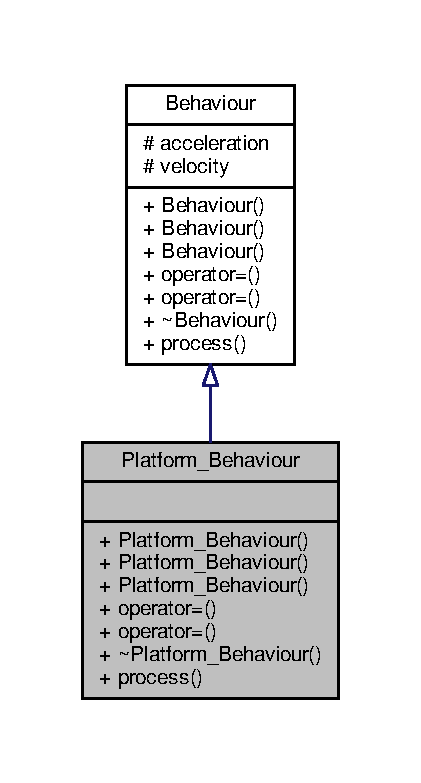
\includegraphics[width=202pt]{classPlatform__Behaviour__inherit__graph}
\end{center}
\end{figure}


Collaboration diagram for Platform\+\_\+\+Behaviour\+:\nopagebreak
\begin{figure}[H]
\begin{center}
\leavevmode
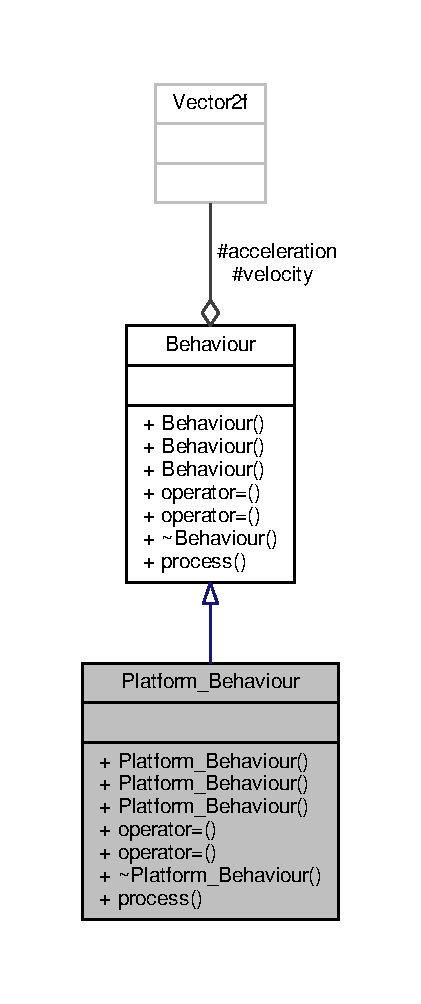
\includegraphics[width=202pt]{classPlatform__Behaviour__coll__graph}
\end{center}
\end{figure}
\subsection*{Public Member Functions}
\begin{DoxyCompactItemize}
\item 
\hyperlink{classPlatform__Behaviour_ae8755b571a2ad73aebb183a6d9ba289b}{Platform\+\_\+\+Behaviour} ()
\begin{DoxyCompactList}\small\item\em Använder \hyperlink{classBehaviour}{Behaviour} konstruktorn. \end{DoxyCompactList}\item 
\hyperlink{classPlatform__Behaviour_aff1ef768551398b8fcae9b765a3b7f44}{Platform\+\_\+\+Behaviour} (\hyperlink{classPlatform__Behaviour}{Platform\+\_\+\+Behaviour} const \&other)=delete
\begin{DoxyCompactList}\small\item\em Copy konstruktor. \end{DoxyCompactList}\item 
\hyperlink{classPlatform__Behaviour_a2f02e74df71cf172120e89ea982ac953}{Platform\+\_\+\+Behaviour} (\hyperlink{classPlatform__Behaviour}{Platform\+\_\+\+Behaviour} \&\&other)=delete
\begin{DoxyCompactList}\small\item\em Move konstruktor. \end{DoxyCompactList}\item 
\hyperlink{classPlatform__Behaviour}{Platform\+\_\+\+Behaviour} \& \hyperlink{classPlatform__Behaviour_aac686ac0c0e8a27ee34d943cf7cf8e99}{operator=} (\hyperlink{classPlatform__Behaviour}{Platform\+\_\+\+Behaviour} const \&rhs)\&=delete
\begin{DoxyCompactList}\small\item\em Copy operator. \end{DoxyCompactList}\item 
\hyperlink{classPlatform__Behaviour}{Platform\+\_\+\+Behaviour} \& \hyperlink{classPlatform__Behaviour_ae5152335d62d30ee7d10d6a7f30b874c}{operator=} (\hyperlink{classPlatform__Behaviour}{Platform\+\_\+\+Behaviour} \&\&rhs)=delete
\begin{DoxyCompactList}\small\item\em Move operator. \end{DoxyCompactList}\item 
\hyperlink{classPlatform__Behaviour_a118ac6c9bd79b02d19d2d8627bee5def}{$\sim$\+Platform\+\_\+\+Behaviour} ()=default
\begin{DoxyCompactList}\small\item\em Default Destruktor. \end{DoxyCompactList}\item 
void \hyperlink{classPlatform__Behaviour_a8a1b458d89bca1e1955aebc2fb44d052}{process} (\hyperlink{classWorld}{World} \&, \hyperlink{classEntity}{Entity} \&, sf\+::\+Time const \&) override
\begin{DoxyCompactList}\small\item\em Funktionen som låter plaformen göra allting. \end{DoxyCompactList}\end{DoxyCompactItemize}
\subsection*{Protected Attributes}
\begin{DoxyCompactItemize}
\item 
sf\+::\+Vector2f \hyperlink{classBehaviour_ac17cf81ceee6a44e8a8ec6ee810c9fd3}{acceleration} \{0.\+0f, 0.\+1f\}
\begin{DoxyCompactList}\small\item\em Variabel för gravitation. \end{DoxyCompactList}\item 
sf\+::\+Vector2f \hyperlink{classBehaviour_a1d52096cf20a59890f7705acbaccf88a}{velocity} \{0.\+0f,0.\+0f\}
\begin{DoxyCompactList}\small\item\em Variabel for hastigheten för entiteten. \end{DoxyCompactList}\end{DoxyCompactItemize}


\subsection{Detailed Description}
\hyperlink{classPlatform__Behaviour}{Platform\+\_\+\+Behaviour} ärver från \hyperlink{classBehaviour}{Behaviour} och tillhandahåller beteendet för platformar. 

Platformars behaviour, de gör ingenting i i dagsläget men måste ha ett behaviour. Detta öppnar också upp möjligheten att skapa mobila platformar om man skulle vilja det. 

\subsection{Constructor \& Destructor Documentation}
\hypertarget{classPlatform__Behaviour_ae8755b571a2ad73aebb183a6d9ba289b}{\index{Platform\+\_\+\+Behaviour@{Platform\+\_\+\+Behaviour}!Platform\+\_\+\+Behaviour@{Platform\+\_\+\+Behaviour}}
\index{Platform\+\_\+\+Behaviour@{Platform\+\_\+\+Behaviour}!Platform\+\_\+\+Behaviour@{Platform\+\_\+\+Behaviour}}
\subsubsection[{Platform\+\_\+\+Behaviour}]{\setlength{\rightskip}{0pt plus 5cm}Platform\+\_\+\+Behaviour\+::\+Platform\+\_\+\+Behaviour (
\begin{DoxyParamCaption}
{}
\end{DoxyParamCaption}
)\hspace{0.3cm}{\ttfamily [inline]}}}\label{classPlatform__Behaviour_ae8755b571a2ad73aebb183a6d9ba289b}


Använder \hyperlink{classBehaviour}{Behaviour} konstruktorn. 

\hypertarget{classPlatform__Behaviour_aff1ef768551398b8fcae9b765a3b7f44}{\index{Platform\+\_\+\+Behaviour@{Platform\+\_\+\+Behaviour}!Platform\+\_\+\+Behaviour@{Platform\+\_\+\+Behaviour}}
\index{Platform\+\_\+\+Behaviour@{Platform\+\_\+\+Behaviour}!Platform\+\_\+\+Behaviour@{Platform\+\_\+\+Behaviour}}
\subsubsection[{Platform\+\_\+\+Behaviour}]{\setlength{\rightskip}{0pt plus 5cm}Platform\+\_\+\+Behaviour\+::\+Platform\+\_\+\+Behaviour (
\begin{DoxyParamCaption}
\item[{{\bf Platform\+\_\+\+Behaviour} const \&}]{other}
\end{DoxyParamCaption}
)\hspace{0.3cm}{\ttfamily [delete]}}}\label{classPlatform__Behaviour_aff1ef768551398b8fcae9b765a3b7f44}


Copy konstruktor. 

\hypertarget{classPlatform__Behaviour_a2f02e74df71cf172120e89ea982ac953}{\index{Platform\+\_\+\+Behaviour@{Platform\+\_\+\+Behaviour}!Platform\+\_\+\+Behaviour@{Platform\+\_\+\+Behaviour}}
\index{Platform\+\_\+\+Behaviour@{Platform\+\_\+\+Behaviour}!Platform\+\_\+\+Behaviour@{Platform\+\_\+\+Behaviour}}
\subsubsection[{Platform\+\_\+\+Behaviour}]{\setlength{\rightskip}{0pt plus 5cm}Platform\+\_\+\+Behaviour\+::\+Platform\+\_\+\+Behaviour (
\begin{DoxyParamCaption}
\item[{{\bf Platform\+\_\+\+Behaviour} \&\&}]{other}
\end{DoxyParamCaption}
)\hspace{0.3cm}{\ttfamily [delete]}}}\label{classPlatform__Behaviour_a2f02e74df71cf172120e89ea982ac953}


Move konstruktor. 

\hypertarget{classPlatform__Behaviour_a118ac6c9bd79b02d19d2d8627bee5def}{\index{Platform\+\_\+\+Behaviour@{Platform\+\_\+\+Behaviour}!````~Platform\+\_\+\+Behaviour@{$\sim$\+Platform\+\_\+\+Behaviour}}
\index{````~Platform\+\_\+\+Behaviour@{$\sim$\+Platform\+\_\+\+Behaviour}!Platform\+\_\+\+Behaviour@{Platform\+\_\+\+Behaviour}}
\subsubsection[{$\sim$\+Platform\+\_\+\+Behaviour}]{\setlength{\rightskip}{0pt plus 5cm}Platform\+\_\+\+Behaviour\+::$\sim$\+Platform\+\_\+\+Behaviour (
\begin{DoxyParamCaption}
{}
\end{DoxyParamCaption}
)\hspace{0.3cm}{\ttfamily [default]}}}\label{classPlatform__Behaviour_a118ac6c9bd79b02d19d2d8627bee5def}


Default Destruktor. 



\subsection{Member Function Documentation}
\hypertarget{classPlatform__Behaviour_aac686ac0c0e8a27ee34d943cf7cf8e99}{\index{Platform\+\_\+\+Behaviour@{Platform\+\_\+\+Behaviour}!operator=@{operator=}}
\index{operator=@{operator=}!Platform\+\_\+\+Behaviour@{Platform\+\_\+\+Behaviour}}
\subsubsection[{operator=}]{\setlength{\rightskip}{0pt plus 5cm}{\bf Platform\+\_\+\+Behaviour}\& Platform\+\_\+\+Behaviour\+::operator= (
\begin{DoxyParamCaption}
\item[{{\bf Platform\+\_\+\+Behaviour} const \&}]{rhs}
\end{DoxyParamCaption}
)\hspace{0.3cm}{\ttfamily [delete]}}}\label{classPlatform__Behaviour_aac686ac0c0e8a27ee34d943cf7cf8e99}


Copy operator. 

\hypertarget{classPlatform__Behaviour_ae5152335d62d30ee7d10d6a7f30b874c}{\index{Platform\+\_\+\+Behaviour@{Platform\+\_\+\+Behaviour}!operator=@{operator=}}
\index{operator=@{operator=}!Platform\+\_\+\+Behaviour@{Platform\+\_\+\+Behaviour}}
\subsubsection[{operator=}]{\setlength{\rightskip}{0pt plus 5cm}{\bf Platform\+\_\+\+Behaviour}\& Platform\+\_\+\+Behaviour\+::operator= (
\begin{DoxyParamCaption}
\item[{{\bf Platform\+\_\+\+Behaviour} \&\&}]{rhs}
\end{DoxyParamCaption}
)\hspace{0.3cm}{\ttfamily [delete]}}}\label{classPlatform__Behaviour_ae5152335d62d30ee7d10d6a7f30b874c}


Move operator. 

\hypertarget{classPlatform__Behaviour_a8a1b458d89bca1e1955aebc2fb44d052}{\index{Platform\+\_\+\+Behaviour@{Platform\+\_\+\+Behaviour}!process@{process}}
\index{process@{process}!Platform\+\_\+\+Behaviour@{Platform\+\_\+\+Behaviour}}
\subsubsection[{process}]{\setlength{\rightskip}{0pt plus 5cm}void Platform\+\_\+\+Behaviour\+::process (
\begin{DoxyParamCaption}
\item[{{\bf World} \&}]{, }
\item[{{\bf Entity} \&}]{, }
\item[{sf\+::\+Time const \&}]{}
\end{DoxyParamCaption}
)\hspace{0.3cm}{\ttfamily [inline]}, {\ttfamily [override]}, {\ttfamily [virtual]}}}\label{classPlatform__Behaviour_a8a1b458d89bca1e1955aebc2fb44d052}


Funktionen som låter plaformen göra allting. 



Implements \hyperlink{classBehaviour_aaa6b4ee24dc3cc546fa4dbb7ba4d20da}{Behaviour}.



\subsection{Member Data Documentation}
\hypertarget{classBehaviour_ac17cf81ceee6a44e8a8ec6ee810c9fd3}{\index{Platform\+\_\+\+Behaviour@{Platform\+\_\+\+Behaviour}!acceleration@{acceleration}}
\index{acceleration@{acceleration}!Platform\+\_\+\+Behaviour@{Platform\+\_\+\+Behaviour}}
\subsubsection[{acceleration}]{\setlength{\rightskip}{0pt plus 5cm}sf\+::\+Vector2f Behaviour\+::acceleration \{0.\+0f, 0.\+1f\}\hspace{0.3cm}{\ttfamily [protected]}, {\ttfamily [inherited]}}}\label{classBehaviour_ac17cf81ceee6a44e8a8ec6ee810c9fd3}


Variabel för gravitation. 

\hypertarget{classBehaviour_a1d52096cf20a59890f7705acbaccf88a}{\index{Platform\+\_\+\+Behaviour@{Platform\+\_\+\+Behaviour}!velocity@{velocity}}
\index{velocity@{velocity}!Platform\+\_\+\+Behaviour@{Platform\+\_\+\+Behaviour}}
\subsubsection[{velocity}]{\setlength{\rightskip}{0pt plus 5cm}sf\+::\+Vector2f Behaviour\+::velocity \{0.\+0f,0.\+0f\}\hspace{0.3cm}{\ttfamily [protected]}, {\ttfamily [inherited]}}}\label{classBehaviour_a1d52096cf20a59890f7705acbaccf88a}


Variabel for hastigheten för entiteten. 



The documentation for this class was generated from the following file\+:\begin{DoxyCompactItemize}
\item 
source/objects/headers/Platform\+\_\+\+Behaviour.\+h\end{DoxyCompactItemize}

\hypertarget{classPlayer}{\section{Player Class Reference}
\label{classPlayer}\index{Player@{Player}}
}


\hyperlink{classPlayer}{Player} ärver från \hyperlink{classEntity}{Entity} och innehåller all information för en entitet av spelartyp.  




{\ttfamily \#include $<$Player.\+h$>$}



Inheritance diagram for Player\+:\nopagebreak
\begin{figure}[H]
\begin{center}
\leavevmode
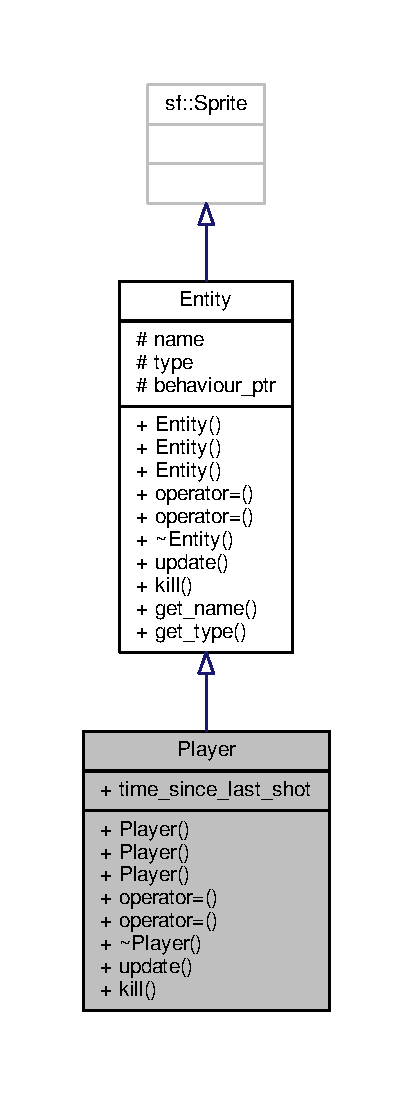
\includegraphics[width=198pt]{classPlayer__inherit__graph}
\end{center}
\end{figure}


Collaboration diagram for Player\+:\nopagebreak
\begin{figure}[H]
\begin{center}
\leavevmode
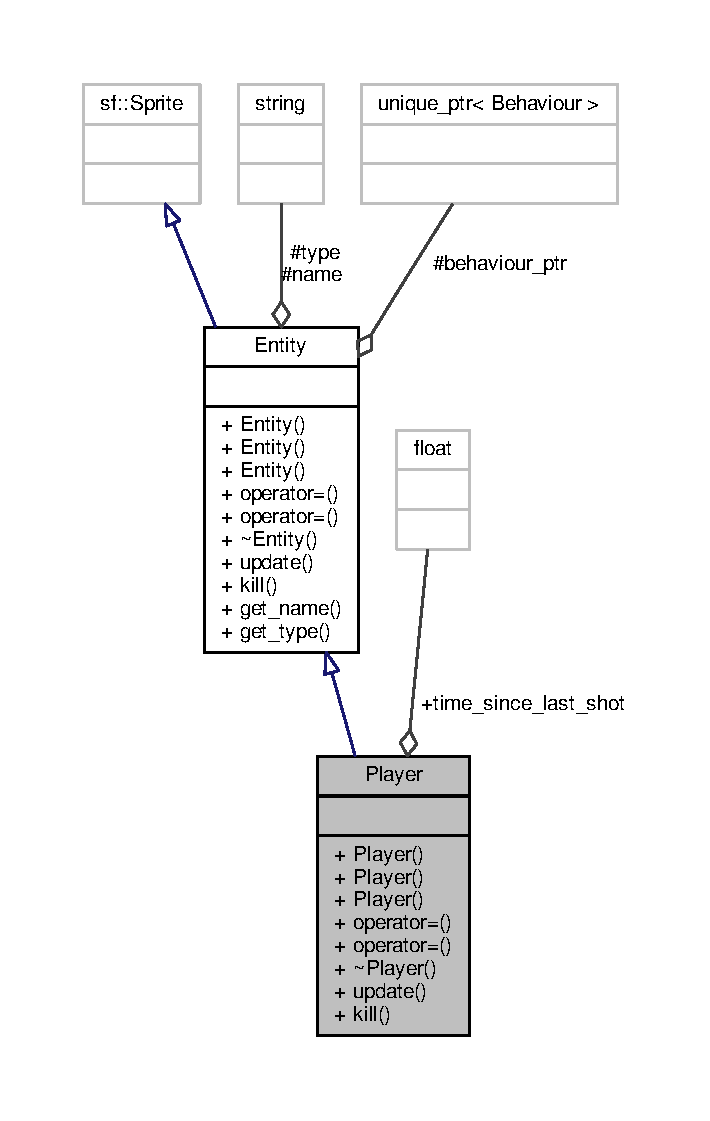
\includegraphics[width=341pt]{classPlayer__coll__graph}
\end{center}
\end{figure}
\subsection*{Public Member Functions}
\begin{DoxyCompactItemize}
\item 
\hyperlink{classPlayer_a2a58e9556edd3dcbedd075055a715948}{Player} (std\+::string, std\+::string, \hyperlink{classBehaviour}{Behaviour} $\ast$, float, float, sf\+::\+Texture const \&, sf\+::\+Int\+Rect, sf\+::\+Color)
\item 
\hyperlink{classPlayer_adde042950f2b58b8f3a3268d1548abd4}{Player} (\hyperlink{classPlayer}{Player} const \&other)=delete
\begin{DoxyCompactList}\small\item\em Copy konstruktor. \end{DoxyCompactList}\item 
\hyperlink{classPlayer_a6beeb56865b114413e5d6a75a9c1e289}{Player} (\hyperlink{classPlayer}{Player} \&\&other)=delete
\begin{DoxyCompactList}\small\item\em Move konstruktor. \end{DoxyCompactList}\item 
\hyperlink{classPlayer}{Player} \& \hyperlink{classPlayer_a1e016eea05266424161f681fe5efca53}{operator=} (\hyperlink{classPlayer}{Player} const \&rhs)\&=delete
\begin{DoxyCompactList}\small\item\em Copy operator. \end{DoxyCompactList}\item 
\hyperlink{classPlayer}{Player} \& \hyperlink{classPlayer_a318b29ff03cd1f7e983a534c5f7f1c37}{operator=} (\hyperlink{classPlayer}{Player} \&\&rhs)=delete
\begin{DoxyCompactList}\small\item\em Move operator. \end{DoxyCompactList}\item 
\hyperlink{classPlayer_a40d3c47b65e9652c363a8fde41f7bbf5}{$\sim$\+Player} ()=default
\begin{DoxyCompactList}\small\item\em Default Destruktor. \end{DoxyCompactList}\item 
void \hyperlink{classPlayer_ad0f6610ee4a9f6d179bf404d1812be54}{update} (\hyperlink{classWorld}{World} \&, sf\+::\+Time const \&) override
\item 
void \hyperlink{classPlayer_ab015823a5707509c3611ff93984100d9}{kill} (\hyperlink{classWorld}{World} \&) override
\begin{DoxyCompactList}\small\item\em Om det här objektet har dödats så kommer kill att göra det genom att informera \hyperlink{classWorld}{World} om det. \end{DoxyCompactList}\item 
std\+::string \hyperlink{classEntity_a75c7e4aad3df2e053ee5b43169509534}{get\+\_\+name} () const 
\begin{DoxyCompactList}\small\item\em Returnerar namnet på entititen. \end{DoxyCompactList}\item 
std\+::string \hyperlink{classEntity_a0e9ef479c1147e21e5bcb338cb858df2}{get\+\_\+type} () const 
\begin{DoxyCompactList}\small\item\em Returnerar typen på entititen. \end{DoxyCompactList}\end{DoxyCompactItemize}
\subsection*{Public Attributes}
\begin{DoxyCompactItemize}
\item 
float \hyperlink{classPlayer_a75e887d14a0eafeeba86bec0e9a8d086}{time\+\_\+since\+\_\+last\+\_\+shot} \{0\}
\begin{DoxyCompactList}\small\item\em En float för att se hur lång tid det var sen spelare senast sköt. \end{DoxyCompactList}\end{DoxyCompactItemize}
\subsection*{Protected Attributes}
\begin{DoxyCompactItemize}
\item 
std\+::string \hyperlink{classEntity_a931b21fbdebb1a5963b4bcab5df128f5}{name}
\begin{DoxyCompactList}\small\item\em Namn. \end{DoxyCompactList}\item 
std\+::string \hyperlink{classEntity_a298a9ebf2474bb00874b5ff6a0d637ef}{type}
\begin{DoxyCompactList}\small\item\em Typ. \end{DoxyCompactList}\item 
std\+::unique\+\_\+ptr$<$ \hyperlink{classBehaviour}{Behaviour} $>$ \hyperlink{classEntity_adb6e36848db24e6d48e6d295e19d3972}{behaviour\+\_\+ptr}
\begin{DoxyCompactList}\small\item\em Unik smart-\/pekare till ett objekt av \hyperlink{classBehaviour}{Behaviour} klassen. \end{DoxyCompactList}\end{DoxyCompactItemize}


\subsection{Detailed Description}
\hyperlink{classPlayer}{Player} ärver från \hyperlink{classEntity}{Entity} och innehåller all information för en entitet av spelartyp. 

\subsection{Constructor \& Destructor Documentation}
\hypertarget{classPlayer_a2a58e9556edd3dcbedd075055a715948}{\index{Player@{Player}!Player@{Player}}
\index{Player@{Player}!Player@{Player}}
\subsubsection[{Player}]{\setlength{\rightskip}{0pt plus 5cm}Player\+::\+Player (
\begin{DoxyParamCaption}
\item[{std\+::string}]{n, }
\item[{std\+::string}]{t, }
\item[{{\bf Behaviour} $\ast$}]{b, }
\item[{float}]{x, }
\item[{float}]{y, }
\item[{sf\+::\+Texture const \&}]{texture, }
\item[{sf\+::\+Int\+Rect}]{size, }
\item[{sf\+::\+Color}]{c}
\end{DoxyParamCaption}
)}}\label{classPlayer_a2a58e9556edd3dcbedd075055a715948}
\hyperlink{classPlayer}{Player} konstruktor som tar in ett namn, en typ, en \hyperlink{classBehaviour}{Behaviour} pekare, en texture, vilken kvadrat som ska ritas ut och vilken färg den ska ha. \hypertarget{classPlayer_adde042950f2b58b8f3a3268d1548abd4}{\index{Player@{Player}!Player@{Player}}
\index{Player@{Player}!Player@{Player}}
\subsubsection[{Player}]{\setlength{\rightskip}{0pt plus 5cm}Player\+::\+Player (
\begin{DoxyParamCaption}
\item[{{\bf Player} const \&}]{other}
\end{DoxyParamCaption}
)\hspace{0.3cm}{\ttfamily [delete]}}}\label{classPlayer_adde042950f2b58b8f3a3268d1548abd4}


Copy konstruktor. 

\hypertarget{classPlayer_a6beeb56865b114413e5d6a75a9c1e289}{\index{Player@{Player}!Player@{Player}}
\index{Player@{Player}!Player@{Player}}
\subsubsection[{Player}]{\setlength{\rightskip}{0pt plus 5cm}Player\+::\+Player (
\begin{DoxyParamCaption}
\item[{{\bf Player} \&\&}]{other}
\end{DoxyParamCaption}
)\hspace{0.3cm}{\ttfamily [delete]}}}\label{classPlayer_a6beeb56865b114413e5d6a75a9c1e289}


Move konstruktor. 

\hypertarget{classPlayer_a40d3c47b65e9652c363a8fde41f7bbf5}{\index{Player@{Player}!````~Player@{$\sim$\+Player}}
\index{````~Player@{$\sim$\+Player}!Player@{Player}}
\subsubsection[{$\sim$\+Player}]{\setlength{\rightskip}{0pt plus 5cm}Player\+::$\sim$\+Player (
\begin{DoxyParamCaption}
{}
\end{DoxyParamCaption}
)\hspace{0.3cm}{\ttfamily [default]}}}\label{classPlayer_a40d3c47b65e9652c363a8fde41f7bbf5}


Default Destruktor. 



\subsection{Member Function Documentation}
\hypertarget{classEntity_a75c7e4aad3df2e053ee5b43169509534}{\index{Player@{Player}!get\+\_\+name@{get\+\_\+name}}
\index{get\+\_\+name@{get\+\_\+name}!Player@{Player}}
\subsubsection[{get\+\_\+name}]{\setlength{\rightskip}{0pt plus 5cm}std\+::string Entity\+::get\+\_\+name (
\begin{DoxyParamCaption}
{}
\end{DoxyParamCaption}
) const\hspace{0.3cm}{\ttfamily [inline]}, {\ttfamily [inherited]}}}\label{classEntity_a75c7e4aad3df2e053ee5b43169509534}


Returnerar namnet på entititen. 

\hypertarget{classEntity_a0e9ef479c1147e21e5bcb338cb858df2}{\index{Player@{Player}!get\+\_\+type@{get\+\_\+type}}
\index{get\+\_\+type@{get\+\_\+type}!Player@{Player}}
\subsubsection[{get\+\_\+type}]{\setlength{\rightskip}{0pt plus 5cm}std\+::string Entity\+::get\+\_\+type (
\begin{DoxyParamCaption}
{}
\end{DoxyParamCaption}
) const\hspace{0.3cm}{\ttfamily [inline]}, {\ttfamily [inherited]}}}\label{classEntity_a0e9ef479c1147e21e5bcb338cb858df2}


Returnerar typen på entititen. 

\hypertarget{classPlayer_ab015823a5707509c3611ff93984100d9}{\index{Player@{Player}!kill@{kill}}
\index{kill@{kill}!Player@{Player}}
\subsubsection[{kill}]{\setlength{\rightskip}{0pt plus 5cm}void Player\+::kill (
\begin{DoxyParamCaption}
\item[{{\bf World} \&}]{w}
\end{DoxyParamCaption}
)\hspace{0.3cm}{\ttfamily [override]}, {\ttfamily [virtual]}}}\label{classPlayer_ab015823a5707509c3611ff93984100d9}


Om det här objektet har dödats så kommer kill att göra det genom att informera \hyperlink{classWorld}{World} om det. 



Implements \hyperlink{classEntity_a3d585a30d7f07c50911485825f5496cd}{Entity}.

\hypertarget{classPlayer_a1e016eea05266424161f681fe5efca53}{\index{Player@{Player}!operator=@{operator=}}
\index{operator=@{operator=}!Player@{Player}}
\subsubsection[{operator=}]{\setlength{\rightskip}{0pt plus 5cm}{\bf Player}\& Player\+::operator= (
\begin{DoxyParamCaption}
\item[{{\bf Player} const \&}]{rhs}
\end{DoxyParamCaption}
)\hspace{0.3cm}{\ttfamily [delete]}}}\label{classPlayer_a1e016eea05266424161f681fe5efca53}


Copy operator. 

\hypertarget{classPlayer_a318b29ff03cd1f7e983a534c5f7f1c37}{\index{Player@{Player}!operator=@{operator=}}
\index{operator=@{operator=}!Player@{Player}}
\subsubsection[{operator=}]{\setlength{\rightskip}{0pt plus 5cm}{\bf Player}\& Player\+::operator= (
\begin{DoxyParamCaption}
\item[{{\bf Player} \&\&}]{rhs}
\end{DoxyParamCaption}
)\hspace{0.3cm}{\ttfamily [delete]}}}\label{classPlayer_a318b29ff03cd1f7e983a534c5f7f1c37}


Move operator. 

\hypertarget{classPlayer_ad0f6610ee4a9f6d179bf404d1812be54}{\index{Player@{Player}!update@{update}}
\index{update@{update}!Player@{Player}}
\subsubsection[{update}]{\setlength{\rightskip}{0pt plus 5cm}void Player\+::update (
\begin{DoxyParamCaption}
\item[{{\bf World} \&}]{world, }
\item[{sf\+::\+Time const \&}]{t}
\end{DoxyParamCaption}
)\hspace{0.3cm}{\ttfamily [override]}, {\ttfamily [virtual]}}}\label{classPlayer_ad0f6610ee4a9f6d179bf404d1812be54}
\hyperlink{classEntity_a180102ac6695559b1f8fcf0aee747802}{Entity\+::update()} override Funktion som kallas av world när det här specifika objektet ska uppdatera sig. Det gör sedan detta genom att t.\+ex. flytta på sig och kolla kollisioner. 

Implements \hyperlink{classEntity_a180102ac6695559b1f8fcf0aee747802}{Entity}.



\subsection{Member Data Documentation}
\hypertarget{classEntity_adb6e36848db24e6d48e6d295e19d3972}{\index{Player@{Player}!behaviour\+\_\+ptr@{behaviour\+\_\+ptr}}
\index{behaviour\+\_\+ptr@{behaviour\+\_\+ptr}!Player@{Player}}
\subsubsection[{behaviour\+\_\+ptr}]{\setlength{\rightskip}{0pt plus 5cm}std\+::unique\+\_\+ptr$<${\bf Behaviour}$>$ Entity\+::behaviour\+\_\+ptr\hspace{0.3cm}{\ttfamily [protected]}, {\ttfamily [inherited]}}}\label{classEntity_adb6e36848db24e6d48e6d295e19d3972}


Unik smart-\/pekare till ett objekt av \hyperlink{classBehaviour}{Behaviour} klassen. 

\hypertarget{classEntity_a931b21fbdebb1a5963b4bcab5df128f5}{\index{Player@{Player}!name@{name}}
\index{name@{name}!Player@{Player}}
\subsubsection[{name}]{\setlength{\rightskip}{0pt plus 5cm}std\+::string Entity\+::name\hspace{0.3cm}{\ttfamily [protected]}, {\ttfamily [inherited]}}}\label{classEntity_a931b21fbdebb1a5963b4bcab5df128f5}


Namn. 

\hypertarget{classPlayer_a75e887d14a0eafeeba86bec0e9a8d086}{\index{Player@{Player}!time\+\_\+since\+\_\+last\+\_\+shot@{time\+\_\+since\+\_\+last\+\_\+shot}}
\index{time\+\_\+since\+\_\+last\+\_\+shot@{time\+\_\+since\+\_\+last\+\_\+shot}!Player@{Player}}
\subsubsection[{time\+\_\+since\+\_\+last\+\_\+shot}]{\setlength{\rightskip}{0pt plus 5cm}float Player\+::time\+\_\+since\+\_\+last\+\_\+shot \{0\}}}\label{classPlayer_a75e887d14a0eafeeba86bec0e9a8d086}


En float för att se hur lång tid det var sen spelare senast sköt. 

\hypertarget{classEntity_a298a9ebf2474bb00874b5ff6a0d637ef}{\index{Player@{Player}!type@{type}}
\index{type@{type}!Player@{Player}}
\subsubsection[{type}]{\setlength{\rightskip}{0pt plus 5cm}std\+::string Entity\+::type\hspace{0.3cm}{\ttfamily [protected]}, {\ttfamily [inherited]}}}\label{classEntity_a298a9ebf2474bb00874b5ff6a0d637ef}


Typ. 



The documentation for this class was generated from the following files\+:\begin{DoxyCompactItemize}
\item 
source/objects/headers/Player.\+h\item 
source/objects/imps/Player.\+cpp\end{DoxyCompactItemize}

\hypertarget{classPlayer__Behaviour}{\section{Player\+\_\+\+Behaviour Class Reference}
\label{classPlayer__Behaviour}\index{Player\+\_\+\+Behaviour@{Player\+\_\+\+Behaviour}}
}


\hyperlink{classPlayer__Behaviour}{Player\+\_\+\+Behaviour} ärver från \hyperlink{classBehaviour}{Behaviour} och tillhandahåller beteendet för spelare.  




{\ttfamily \#include $<$Player\+\_\+\+Behaviour.\+h$>$}



Inheritance diagram for Player\+\_\+\+Behaviour\+:\nopagebreak
\begin{figure}[H]
\begin{center}
\leavevmode
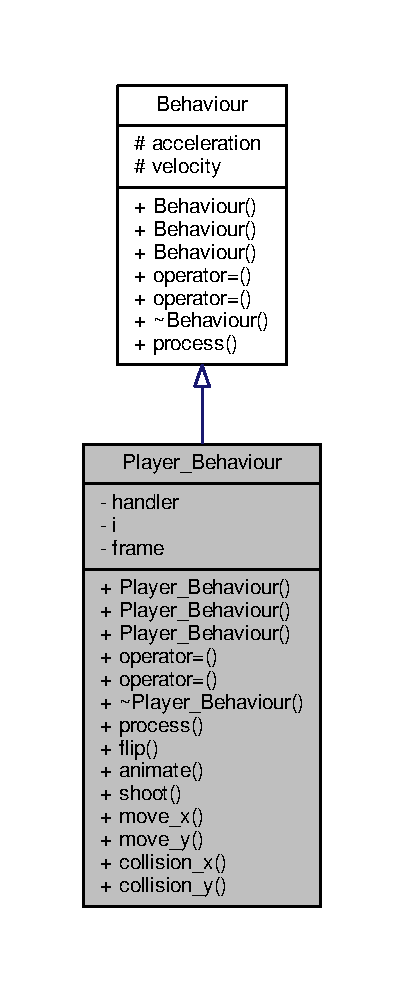
\includegraphics[width=194pt]{classPlayer__Behaviour__inherit__graph}
\end{center}
\end{figure}


Collaboration diagram for Player\+\_\+\+Behaviour\+:\nopagebreak
\begin{figure}[H]
\begin{center}
\leavevmode
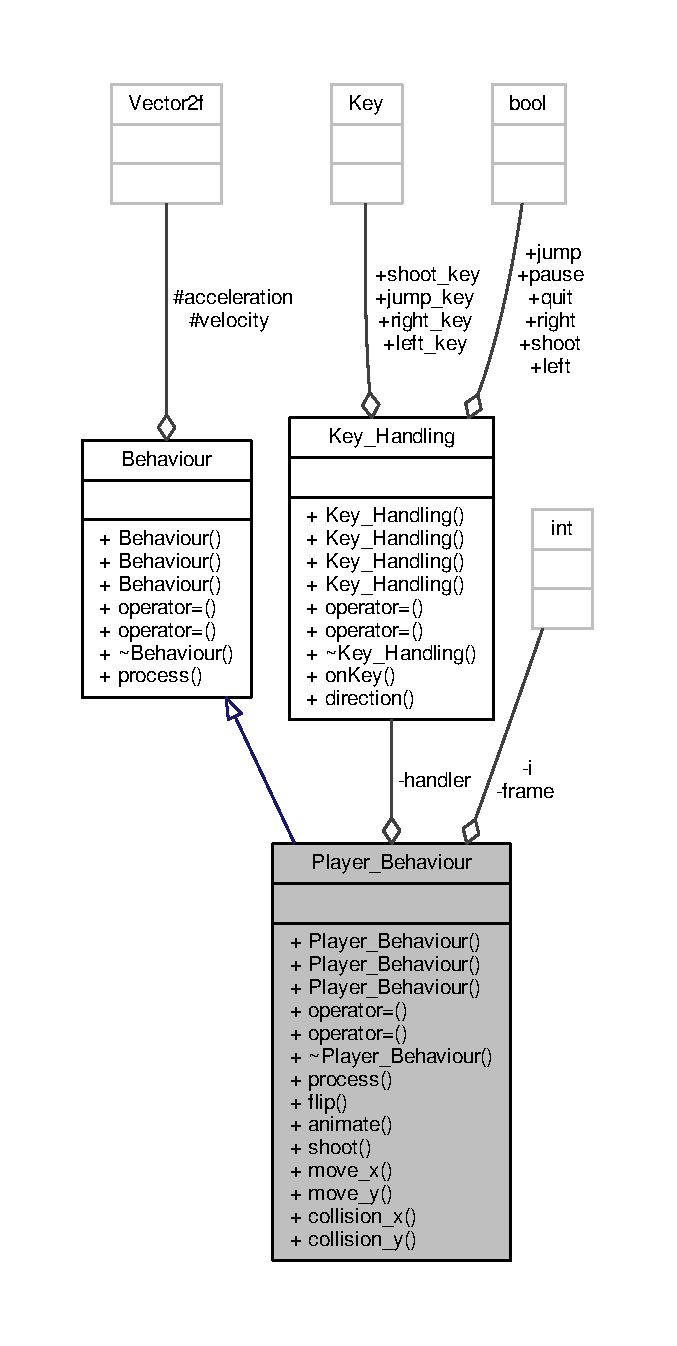
\includegraphics[height=550pt]{classPlayer__Behaviour__coll__graph}
\end{center}
\end{figure}
\subsection*{Public Member Functions}
\begin{DoxyCompactItemize}
\item 
\hyperlink{classPlayer__Behaviour_af2ac9398d19327733bfc83e672782580}{Player\+\_\+\+Behaviour} (\hyperlink{classKey__Handling}{Key\+\_\+\+Handling} \&)
\begin{DoxyCompactList}\small\item\em En vanlig konstruktor som tar in ett referens till en \hyperlink{classKey__Handling}{Key\+\_\+\+Handling}. \end{DoxyCompactList}\item 
\hyperlink{classPlayer__Behaviour_a4f7527788db7e0077f46a5c3f80639fa}{Player\+\_\+\+Behaviour} (\hyperlink{classPlayer__Behaviour}{Player\+\_\+\+Behaviour} const \&other)=delete
\begin{DoxyCompactList}\small\item\em Copy konstruktor. \end{DoxyCompactList}\item 
\hyperlink{classPlayer__Behaviour_a8060453cd5b18254154d986bd5c31a0b}{Player\+\_\+\+Behaviour} (\hyperlink{classPlayer__Behaviour}{Player\+\_\+\+Behaviour} \&\&other)=delete
\begin{DoxyCompactList}\small\item\em Move konstruktor. \end{DoxyCompactList}\item 
\hyperlink{classPlayer__Behaviour}{Player\+\_\+\+Behaviour} \& \hyperlink{classPlayer__Behaviour_a313984f091f92701d0a890e8643398a8}{operator=} (\hyperlink{classPlayer__Behaviour}{Player\+\_\+\+Behaviour} const \&rhs)\&=delete
\begin{DoxyCompactList}\small\item\em Copy operator. \end{DoxyCompactList}\item 
\hyperlink{classPlayer__Behaviour}{Player\+\_\+\+Behaviour} \& \hyperlink{classPlayer__Behaviour_acccc40229c43598189255bac420e0f8f}{operator=} (\hyperlink{classPlayer__Behaviour}{Player\+\_\+\+Behaviour} \&\&rhs)=delete
\begin{DoxyCompactList}\small\item\em Move operator. \end{DoxyCompactList}\item 
\hyperlink{classPlayer__Behaviour_a776d896d15ebce163770778d192404c4}{$\sim$\+Player\+\_\+\+Behaviour} ()=default
\begin{DoxyCompactList}\small\item\em Default Destruktor. \end{DoxyCompactList}\item 
void \hyperlink{classPlayer__Behaviour_aa88f449e71197691e1166e985f165fa6}{process} (\hyperlink{classWorld}{World} \&, \hyperlink{classEntity}{Entity} \&, sf\+::\+Time const \&) override
\begin{DoxyCompactList}\small\item\em Funktionen som låter player utföra sina actions. \end{DoxyCompactList}\item 
void \hyperlink{classPlayer__Behaviour_a286c0e64639b320704e3c0ea6b7dafd9}{flip} (\hyperlink{classEntity}{Entity} \&, sf\+::\+Vector2f const \&)
\begin{DoxyCompactList}\small\item\em Funktionen flipar spriten för enemy baserat på vilket håll den rör sig. \end{DoxyCompactList}\item 
void \hyperlink{classPlayer__Behaviour_a0731770843676863bceed9b7fe1033c7}{animate} (\hyperlink{classWorld}{World} \&, \hyperlink{classEntity}{Entity} \&)
\begin{DoxyCompactList}\small\item\em En animeringsklocka som ändrar på texturens visningskvadrat. \end{DoxyCompactList}\item 
void \hyperlink{classPlayer__Behaviour_ab2f7b0265a09d1f645231990c3ac3a27}{shoot} (\hyperlink{classWorld}{World} \&, \hyperlink{classPlayer}{Player} \&, sf\+::\+Time)
\item 
void \hyperlink{classPlayer__Behaviour_a6a440d70c136fb818db8606230bdcf1b}{move\+\_\+x} (\hyperlink{classEntity}{Entity} \&, sf\+::\+Vector2f const \&, sf\+::\+Time)
\begin{DoxyCompactList}\small\item\em Förflyttning i x-\/led. \end{DoxyCompactList}\item 
void \hyperlink{classPlayer__Behaviour_aca6d6268d1c798e0af747ca708393a76}{move\+\_\+y} (\hyperlink{classEntity}{Entity} \&, sf\+::\+Vector2f const \&, sf\+::\+Time)
\begin{DoxyCompactList}\small\item\em Förflyttning i y-\/led. \end{DoxyCompactList}\item 
void \hyperlink{classPlayer__Behaviour_a9fe9aa64239db57c6eaeb17e91d750be}{collision\+\_\+x} (\hyperlink{classWorld}{World} \&, \hyperlink{classEntity}{Entity} \&)
\begin{DoxyCompactList}\small\item\em Kollisionshantering i x-\/led. \end{DoxyCompactList}\item 
void \hyperlink{classPlayer__Behaviour_a9cec7f10ae6eb9e64d346247e3b56638}{collision\+\_\+y} (\hyperlink{classWorld}{World} \&, \hyperlink{classEntity}{Entity} \&)
\begin{DoxyCompactList}\small\item\em Kollisionshantering i y-\/led. \end{DoxyCompactList}\end{DoxyCompactItemize}
\subsection*{Protected Attributes}
\begin{DoxyCompactItemize}
\item 
sf\+::\+Vector2f \hyperlink{classBehaviour_ac17cf81ceee6a44e8a8ec6ee810c9fd3}{acceleration} \{0.\+0f, 0.\+1f\}
\begin{DoxyCompactList}\small\item\em Variabel för gravitation. \end{DoxyCompactList}\item 
sf\+::\+Vector2f \hyperlink{classBehaviour_a1d52096cf20a59890f7705acbaccf88a}{velocity} \{0.\+0f,0.\+0f\}
\begin{DoxyCompactList}\small\item\em Variabel for hastigheten för entiteten. \end{DoxyCompactList}\end{DoxyCompactItemize}
\subsection*{Private Attributes}
\begin{DoxyCompactItemize}
\item 
\hyperlink{classKey__Handling}{Key\+\_\+\+Handling} \& \hyperlink{classPlayer__Behaviour_a14e943931e401609e8182340b4a7273c}{handler}
\item 
int \hyperlink{classPlayer__Behaviour_a349e59d8a094c3f5b7263471135686bc}{i} \{0\}
\begin{DoxyCompactList}\small\item\em Variabel för att simulera en klocka. \end{DoxyCompactList}\item 
int \hyperlink{classPlayer__Behaviour_af51ca380d3847dfeee6636abf7f5a6a9}{frame} \{0\}
\begin{DoxyCompactList}\small\item\em Vilken frame som ska ritas ut. \end{DoxyCompactList}\end{DoxyCompactItemize}


\subsection{Detailed Description}
\hyperlink{classPlayer__Behaviour}{Player\+\_\+\+Behaviour} ärver från \hyperlink{classBehaviour}{Behaviour} och tillhandahåller beteendet för spelare. 

\hyperlink{classPlayer__Behaviour}{Player\+\_\+\+Behaviour} ärver allting från \hyperlink{classBehaviour}{Behaviour} och låter spelaren interagera med spelvärlden. Detta genom att flytta spelare, kollidera med objekt, skjuta projektiler, animera spelaren och flippa spelarens sprite baserat på var spelaren går. 

\subsection{Constructor \& Destructor Documentation}
\hypertarget{classPlayer__Behaviour_af2ac9398d19327733bfc83e672782580}{\index{Player\+\_\+\+Behaviour@{Player\+\_\+\+Behaviour}!Player\+\_\+\+Behaviour@{Player\+\_\+\+Behaviour}}
\index{Player\+\_\+\+Behaviour@{Player\+\_\+\+Behaviour}!Player\+\_\+\+Behaviour@{Player\+\_\+\+Behaviour}}
\subsubsection[{Player\+\_\+\+Behaviour}]{\setlength{\rightskip}{0pt plus 5cm}Player\+\_\+\+Behaviour\+::\+Player\+\_\+\+Behaviour (
\begin{DoxyParamCaption}
\item[{{\bf Key\+\_\+\+Handling} \&}]{key\+\_\+handler}
\end{DoxyParamCaption}
)}}\label{classPlayer__Behaviour_af2ac9398d19327733bfc83e672782580}


En vanlig konstruktor som tar in ett referens till en \hyperlink{classKey__Handling}{Key\+\_\+\+Handling}. 

\hypertarget{classPlayer__Behaviour_a4f7527788db7e0077f46a5c3f80639fa}{\index{Player\+\_\+\+Behaviour@{Player\+\_\+\+Behaviour}!Player\+\_\+\+Behaviour@{Player\+\_\+\+Behaviour}}
\index{Player\+\_\+\+Behaviour@{Player\+\_\+\+Behaviour}!Player\+\_\+\+Behaviour@{Player\+\_\+\+Behaviour}}
\subsubsection[{Player\+\_\+\+Behaviour}]{\setlength{\rightskip}{0pt plus 5cm}Player\+\_\+\+Behaviour\+::\+Player\+\_\+\+Behaviour (
\begin{DoxyParamCaption}
\item[{{\bf Player\+\_\+\+Behaviour} const \&}]{other}
\end{DoxyParamCaption}
)\hspace{0.3cm}{\ttfamily [delete]}}}\label{classPlayer__Behaviour_a4f7527788db7e0077f46a5c3f80639fa}


Copy konstruktor. 

\hypertarget{classPlayer__Behaviour_a8060453cd5b18254154d986bd5c31a0b}{\index{Player\+\_\+\+Behaviour@{Player\+\_\+\+Behaviour}!Player\+\_\+\+Behaviour@{Player\+\_\+\+Behaviour}}
\index{Player\+\_\+\+Behaviour@{Player\+\_\+\+Behaviour}!Player\+\_\+\+Behaviour@{Player\+\_\+\+Behaviour}}
\subsubsection[{Player\+\_\+\+Behaviour}]{\setlength{\rightskip}{0pt plus 5cm}Player\+\_\+\+Behaviour\+::\+Player\+\_\+\+Behaviour (
\begin{DoxyParamCaption}
\item[{{\bf Player\+\_\+\+Behaviour} \&\&}]{other}
\end{DoxyParamCaption}
)\hspace{0.3cm}{\ttfamily [delete]}}}\label{classPlayer__Behaviour_a8060453cd5b18254154d986bd5c31a0b}


Move konstruktor. 

\hypertarget{classPlayer__Behaviour_a776d896d15ebce163770778d192404c4}{\index{Player\+\_\+\+Behaviour@{Player\+\_\+\+Behaviour}!````~Player\+\_\+\+Behaviour@{$\sim$\+Player\+\_\+\+Behaviour}}
\index{````~Player\+\_\+\+Behaviour@{$\sim$\+Player\+\_\+\+Behaviour}!Player\+\_\+\+Behaviour@{Player\+\_\+\+Behaviour}}
\subsubsection[{$\sim$\+Player\+\_\+\+Behaviour}]{\setlength{\rightskip}{0pt plus 5cm}Player\+\_\+\+Behaviour\+::$\sim$\+Player\+\_\+\+Behaviour (
\begin{DoxyParamCaption}
{}
\end{DoxyParamCaption}
)\hspace{0.3cm}{\ttfamily [default]}}}\label{classPlayer__Behaviour_a776d896d15ebce163770778d192404c4}


Default Destruktor. 



\subsection{Member Function Documentation}
\hypertarget{classPlayer__Behaviour_a0731770843676863bceed9b7fe1033c7}{\index{Player\+\_\+\+Behaviour@{Player\+\_\+\+Behaviour}!animate@{animate}}
\index{animate@{animate}!Player\+\_\+\+Behaviour@{Player\+\_\+\+Behaviour}}
\subsubsection[{animate}]{\setlength{\rightskip}{0pt plus 5cm}void Player\+\_\+\+Behaviour\+::animate (
\begin{DoxyParamCaption}
\item[{{\bf World} \&}]{world, }
\item[{{\bf Entity} \&}]{owner}
\end{DoxyParamCaption}
)}}\label{classPlayer__Behaviour_a0731770843676863bceed9b7fe1033c7}


En animeringsklocka som ändrar på texturens visningskvadrat. 

\hypertarget{classPlayer__Behaviour_a9fe9aa64239db57c6eaeb17e91d750be}{\index{Player\+\_\+\+Behaviour@{Player\+\_\+\+Behaviour}!collision\+\_\+x@{collision\+\_\+x}}
\index{collision\+\_\+x@{collision\+\_\+x}!Player\+\_\+\+Behaviour@{Player\+\_\+\+Behaviour}}
\subsubsection[{collision\+\_\+x}]{\setlength{\rightskip}{0pt plus 5cm}void Player\+\_\+\+Behaviour\+::collision\+\_\+x (
\begin{DoxyParamCaption}
\item[{{\bf World} \&}]{world, }
\item[{{\bf Entity} \&}]{owner}
\end{DoxyParamCaption}
)}}\label{classPlayer__Behaviour_a9fe9aa64239db57c6eaeb17e91d750be}


Kollisionshantering i x-\/led. 

\hypertarget{classPlayer__Behaviour_a9cec7f10ae6eb9e64d346247e3b56638}{\index{Player\+\_\+\+Behaviour@{Player\+\_\+\+Behaviour}!collision\+\_\+y@{collision\+\_\+y}}
\index{collision\+\_\+y@{collision\+\_\+y}!Player\+\_\+\+Behaviour@{Player\+\_\+\+Behaviour}}
\subsubsection[{collision\+\_\+y}]{\setlength{\rightskip}{0pt plus 5cm}void Player\+\_\+\+Behaviour\+::collision\+\_\+y (
\begin{DoxyParamCaption}
\item[{{\bf World} \&}]{world, }
\item[{{\bf Entity} \&}]{owner}
\end{DoxyParamCaption}
)}}\label{classPlayer__Behaviour_a9cec7f10ae6eb9e64d346247e3b56638}


Kollisionshantering i y-\/led. 

\hypertarget{classPlayer__Behaviour_a286c0e64639b320704e3c0ea6b7dafd9}{\index{Player\+\_\+\+Behaviour@{Player\+\_\+\+Behaviour}!flip@{flip}}
\index{flip@{flip}!Player\+\_\+\+Behaviour@{Player\+\_\+\+Behaviour}}
\subsubsection[{flip}]{\setlength{\rightskip}{0pt plus 5cm}void Player\+\_\+\+Behaviour\+::flip (
\begin{DoxyParamCaption}
\item[{{\bf Entity} \&}]{owner, }
\item[{sf\+::\+Vector2f const \&}]{dir}
\end{DoxyParamCaption}
)}}\label{classPlayer__Behaviour_a286c0e64639b320704e3c0ea6b7dafd9}


Funktionen flipar spriten för enemy baserat på vilket håll den rör sig. 

\hypertarget{classPlayer__Behaviour_a6a440d70c136fb818db8606230bdcf1b}{\index{Player\+\_\+\+Behaviour@{Player\+\_\+\+Behaviour}!move\+\_\+x@{move\+\_\+x}}
\index{move\+\_\+x@{move\+\_\+x}!Player\+\_\+\+Behaviour@{Player\+\_\+\+Behaviour}}
\subsubsection[{move\+\_\+x}]{\setlength{\rightskip}{0pt plus 5cm}void Player\+\_\+\+Behaviour\+::move\+\_\+x (
\begin{DoxyParamCaption}
\item[{{\bf Entity} \&}]{owner, }
\item[{sf\+::\+Vector2f const \&}]{dir, }
\item[{sf\+::\+Time}]{t}
\end{DoxyParamCaption}
)}}\label{classPlayer__Behaviour_a6a440d70c136fb818db8606230bdcf1b}


Förflyttning i x-\/led. 

\hypertarget{classPlayer__Behaviour_aca6d6268d1c798e0af747ca708393a76}{\index{Player\+\_\+\+Behaviour@{Player\+\_\+\+Behaviour}!move\+\_\+y@{move\+\_\+y}}
\index{move\+\_\+y@{move\+\_\+y}!Player\+\_\+\+Behaviour@{Player\+\_\+\+Behaviour}}
\subsubsection[{move\+\_\+y}]{\setlength{\rightskip}{0pt plus 5cm}void Player\+\_\+\+Behaviour\+::move\+\_\+y (
\begin{DoxyParamCaption}
\item[{{\bf Entity} \&}]{owner, }
\item[{sf\+::\+Vector2f const \&}]{dir, }
\item[{sf\+::\+Time}]{t}
\end{DoxyParamCaption}
)}}\label{classPlayer__Behaviour_aca6d6268d1c798e0af747ca708393a76}


Förflyttning i y-\/led. 

\hypertarget{classPlayer__Behaviour_a313984f091f92701d0a890e8643398a8}{\index{Player\+\_\+\+Behaviour@{Player\+\_\+\+Behaviour}!operator=@{operator=}}
\index{operator=@{operator=}!Player\+\_\+\+Behaviour@{Player\+\_\+\+Behaviour}}
\subsubsection[{operator=}]{\setlength{\rightskip}{0pt plus 5cm}{\bf Player\+\_\+\+Behaviour}\& Player\+\_\+\+Behaviour\+::operator= (
\begin{DoxyParamCaption}
\item[{{\bf Player\+\_\+\+Behaviour} const \&}]{rhs}
\end{DoxyParamCaption}
)\hspace{0.3cm}{\ttfamily [delete]}}}\label{classPlayer__Behaviour_a313984f091f92701d0a890e8643398a8}


Copy operator. 

\hypertarget{classPlayer__Behaviour_acccc40229c43598189255bac420e0f8f}{\index{Player\+\_\+\+Behaviour@{Player\+\_\+\+Behaviour}!operator=@{operator=}}
\index{operator=@{operator=}!Player\+\_\+\+Behaviour@{Player\+\_\+\+Behaviour}}
\subsubsection[{operator=}]{\setlength{\rightskip}{0pt plus 5cm}{\bf Player\+\_\+\+Behaviour}\& Player\+\_\+\+Behaviour\+::operator= (
\begin{DoxyParamCaption}
\item[{{\bf Player\+\_\+\+Behaviour} \&\&}]{rhs}
\end{DoxyParamCaption}
)\hspace{0.3cm}{\ttfamily [delete]}}}\label{classPlayer__Behaviour_acccc40229c43598189255bac420e0f8f}


Move operator. 

\hypertarget{classPlayer__Behaviour_aa88f449e71197691e1166e985f165fa6}{\index{Player\+\_\+\+Behaviour@{Player\+\_\+\+Behaviour}!process@{process}}
\index{process@{process}!Player\+\_\+\+Behaviour@{Player\+\_\+\+Behaviour}}
\subsubsection[{process}]{\setlength{\rightskip}{0pt plus 5cm}void Player\+\_\+\+Behaviour\+::process (
\begin{DoxyParamCaption}
\item[{{\bf World} \&}]{world, }
\item[{{\bf Entity} \&}]{owner, }
\item[{sf\+::\+Time const \&}]{t}
\end{DoxyParamCaption}
)\hspace{0.3cm}{\ttfamily [override]}, {\ttfamily [virtual]}}}\label{classPlayer__Behaviour_aa88f449e71197691e1166e985f165fa6}


Funktionen som låter player utföra sina actions. 



Implements \hyperlink{classBehaviour_aaa6b4ee24dc3cc546fa4dbb7ba4d20da}{Behaviour}.

\hypertarget{classPlayer__Behaviour_ab2f7b0265a09d1f645231990c3ac3a27}{\index{Player\+\_\+\+Behaviour@{Player\+\_\+\+Behaviour}!shoot@{shoot}}
\index{shoot@{shoot}!Player\+\_\+\+Behaviour@{Player\+\_\+\+Behaviour}}
\subsubsection[{shoot}]{\setlength{\rightskip}{0pt plus 5cm}void Player\+\_\+\+Behaviour\+::shoot (
\begin{DoxyParamCaption}
\item[{{\bf World} \&}]{world, }
\item[{{\bf Player} \&}]{owner, }
\item[{sf\+::\+Time}]{t}
\end{DoxyParamCaption}
)}}\label{classPlayer__Behaviour_ab2f7b0265a09d1f645231990c3ac3a27}
Funktionen som låter spelare skjuta. Den ändrar på spelarens textur för att kunna animera skjutande. 

\subsection{Member Data Documentation}
\hypertarget{classBehaviour_ac17cf81ceee6a44e8a8ec6ee810c9fd3}{\index{Player\+\_\+\+Behaviour@{Player\+\_\+\+Behaviour}!acceleration@{acceleration}}
\index{acceleration@{acceleration}!Player\+\_\+\+Behaviour@{Player\+\_\+\+Behaviour}}
\subsubsection[{acceleration}]{\setlength{\rightskip}{0pt plus 5cm}sf\+::\+Vector2f Behaviour\+::acceleration \{0.\+0f, 0.\+1f\}\hspace{0.3cm}{\ttfamily [protected]}, {\ttfamily [inherited]}}}\label{classBehaviour_ac17cf81ceee6a44e8a8ec6ee810c9fd3}


Variabel för gravitation. 

\hypertarget{classPlayer__Behaviour_af51ca380d3847dfeee6636abf7f5a6a9}{\index{Player\+\_\+\+Behaviour@{Player\+\_\+\+Behaviour}!frame@{frame}}
\index{frame@{frame}!Player\+\_\+\+Behaviour@{Player\+\_\+\+Behaviour}}
\subsubsection[{frame}]{\setlength{\rightskip}{0pt plus 5cm}int Player\+\_\+\+Behaviour\+::frame \{0\}\hspace{0.3cm}{\ttfamily [private]}}}\label{classPlayer__Behaviour_af51ca380d3847dfeee6636abf7f5a6a9}


Vilken frame som ska ritas ut. 

\hypertarget{classPlayer__Behaviour_a14e943931e401609e8182340b4a7273c}{\index{Player\+\_\+\+Behaviour@{Player\+\_\+\+Behaviour}!handler@{handler}}
\index{handler@{handler}!Player\+\_\+\+Behaviour@{Player\+\_\+\+Behaviour}}
\subsubsection[{handler}]{\setlength{\rightskip}{0pt plus 5cm}{\bf Key\+\_\+\+Handling}\& Player\+\_\+\+Behaviour\+::handler\hspace{0.3cm}{\ttfamily [private]}}}\label{classPlayer__Behaviour_a14e943931e401609e8182340b4a7273c}
En variabel som visar vilken \hyperlink{classKey__Handling}{Key\+\_\+\+Handling} \hyperlink{classPlayer__Behaviour}{Player\+\_\+\+Behaviour} objektet ska lyssna på. \hypertarget{classPlayer__Behaviour_a349e59d8a094c3f5b7263471135686bc}{\index{Player\+\_\+\+Behaviour@{Player\+\_\+\+Behaviour}!i@{i}}
\index{i@{i}!Player\+\_\+\+Behaviour@{Player\+\_\+\+Behaviour}}
\subsubsection[{i}]{\setlength{\rightskip}{0pt plus 5cm}int Player\+\_\+\+Behaviour\+::i \{0\}\hspace{0.3cm}{\ttfamily [private]}}}\label{classPlayer__Behaviour_a349e59d8a094c3f5b7263471135686bc}


Variabel för att simulera en klocka. 

\hypertarget{classBehaviour_a1d52096cf20a59890f7705acbaccf88a}{\index{Player\+\_\+\+Behaviour@{Player\+\_\+\+Behaviour}!velocity@{velocity}}
\index{velocity@{velocity}!Player\+\_\+\+Behaviour@{Player\+\_\+\+Behaviour}}
\subsubsection[{velocity}]{\setlength{\rightskip}{0pt plus 5cm}sf\+::\+Vector2f Behaviour\+::velocity \{0.\+0f,0.\+0f\}\hspace{0.3cm}{\ttfamily [protected]}, {\ttfamily [inherited]}}}\label{classBehaviour_a1d52096cf20a59890f7705acbaccf88a}


Variabel for hastigheten för entiteten. 



The documentation for this class was generated from the following files\+:\begin{DoxyCompactItemize}
\item 
source/objects/headers/Player\+\_\+\+Behaviour.\+h\item 
source/objects/imps/Player\+\_\+\+Behaviour.\+cpp\end{DoxyCompactItemize}

\hypertarget{classProjectile}{\section{Projectile Class Reference}
\label{classProjectile}\index{Projectile@{Projectile}}
}


\hyperlink{classProjectile}{Projectile} ärver från \hyperlink{classEntity}{Entity} och innehåller all information för en entitet av projektil typ.  




{\ttfamily \#include $<$Projectile.\+h$>$}



Inheritance diagram for Projectile\+:\nopagebreak
\begin{figure}[H]
\begin{center}
\leavevmode
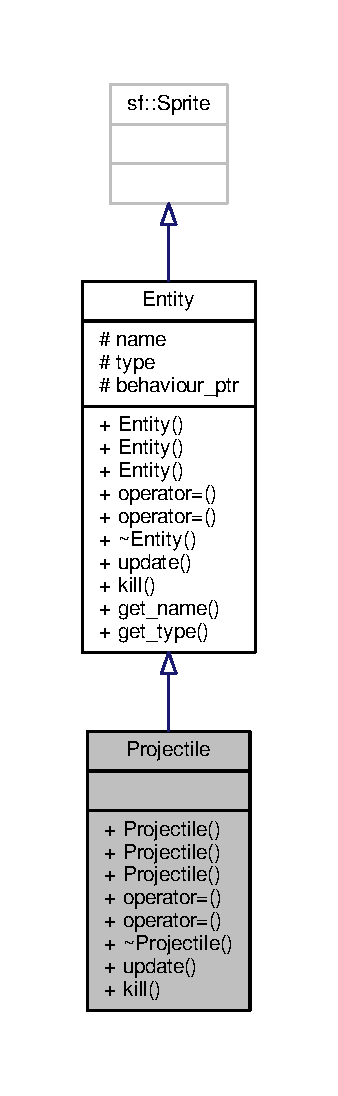
\includegraphics[width=162pt]{classProjectile__inherit__graph}
\end{center}
\end{figure}


Collaboration diagram for Projectile\+:\nopagebreak
\begin{figure}[H]
\begin{center}
\leavevmode
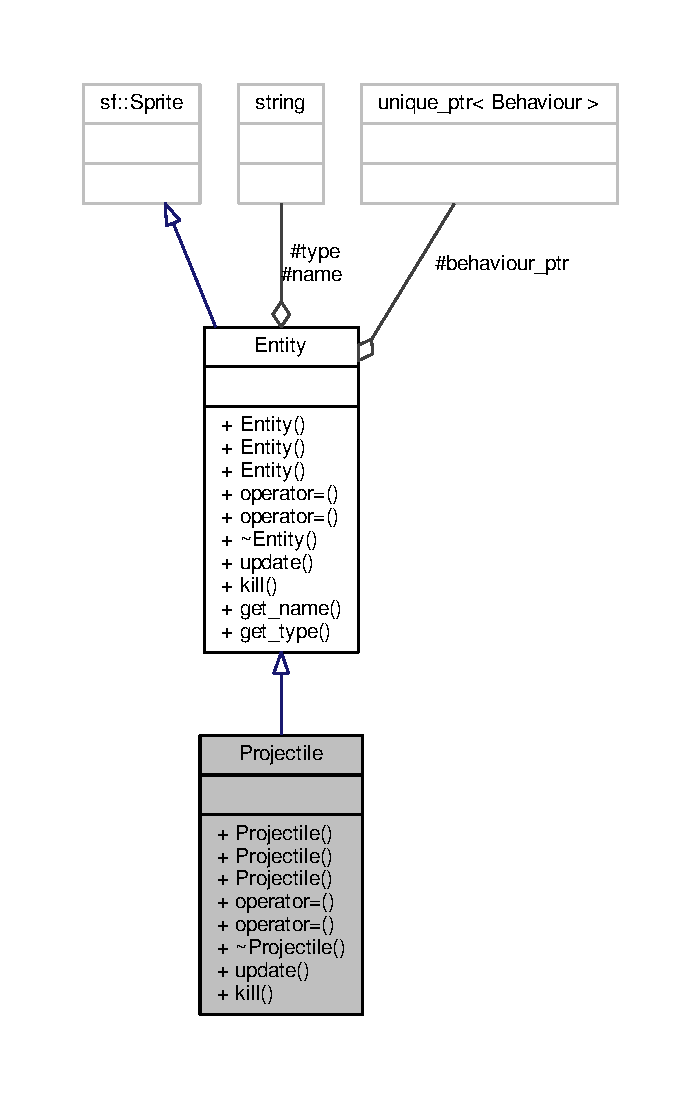
\includegraphics[width=336pt]{classProjectile__coll__graph}
\end{center}
\end{figure}
\subsection*{Public Member Functions}
\begin{DoxyCompactItemize}
\item 
\hyperlink{classProjectile_a5898ed148789733b461db3b662cb2e12}{Projectile} (std\+::string n, std\+::string t, \hyperlink{classBehaviour}{Behaviour} $\ast$b, float x, float y, sf\+::\+Texture const \&, sf\+::\+Int\+Rect)
\item 
\hyperlink{classProjectile_ab1b6aba20a26659c6e48ca04fd6fcdd9}{Projectile} (\hyperlink{classProjectile}{Projectile} const \&other)=delete
\begin{DoxyCompactList}\small\item\em Copy konstruktor. \end{DoxyCompactList}\item 
\hyperlink{classProjectile_ada97affd8ca4c6e99b8bd2e8f2acd4ef}{Projectile} (\hyperlink{classProjectile}{Projectile} \&\&other)=delete
\begin{DoxyCompactList}\small\item\em Move konstruktor. \end{DoxyCompactList}\item 
\hyperlink{classProjectile}{Projectile} \& \hyperlink{classProjectile_ad60195da40c606e67b50ad334c59459a}{operator=} (\hyperlink{classProjectile}{Projectile} const \&rhs)\&=delete
\begin{DoxyCompactList}\small\item\em Copy operator. \end{DoxyCompactList}\item 
\hyperlink{classProjectile}{Projectile} \& \hyperlink{classProjectile_a6de99820546dbd177ee4c20cf90b7bce}{operator=} (\hyperlink{classProjectile}{Projectile} \&\&rhs)=delete
\begin{DoxyCompactList}\small\item\em Move operator. \end{DoxyCompactList}\item 
\hyperlink{classProjectile_a74de98e362b6944a533663db8a45340c}{$\sim$\+Projectile} ()=default
\begin{DoxyCompactList}\small\item\em Default Destruktor. \end{DoxyCompactList}\item 
void \hyperlink{classProjectile_a48d52d5d9db6e3af4aae8ded6afa6544}{update} (\hyperlink{classWorld}{World} \&, sf\+::\+Time const \&t) override
\item 
void \hyperlink{classProjectile_a10d7ca9bb3d022246196572d008f1d59}{kill} (\hyperlink{classWorld}{World} \&w) override
\begin{DoxyCompactList}\small\item\em Om det här objektet har dödats så kommer kill att göra det genom att informera \hyperlink{classWorld}{World} om det. \end{DoxyCompactList}\item 
std\+::string \hyperlink{classEntity_a75c7e4aad3df2e053ee5b43169509534}{get\+\_\+name} () const 
\begin{DoxyCompactList}\small\item\em Returnerar namnet på entititen. \end{DoxyCompactList}\item 
std\+::string \hyperlink{classEntity_a0e9ef479c1147e21e5bcb338cb858df2}{get\+\_\+type} () const 
\begin{DoxyCompactList}\small\item\em Returnerar typen på entititen. \end{DoxyCompactList}\end{DoxyCompactItemize}
\subsection*{Protected Attributes}
\begin{DoxyCompactItemize}
\item 
std\+::string \hyperlink{classEntity_a931b21fbdebb1a5963b4bcab5df128f5}{name}
\begin{DoxyCompactList}\small\item\em Namn. \end{DoxyCompactList}\item 
std\+::string \hyperlink{classEntity_a298a9ebf2474bb00874b5ff6a0d637ef}{type}
\begin{DoxyCompactList}\small\item\em Typ. \end{DoxyCompactList}\item 
std\+::unique\+\_\+ptr$<$ \hyperlink{classBehaviour}{Behaviour} $>$ \hyperlink{classEntity_adb6e36848db24e6d48e6d295e19d3972}{behaviour\+\_\+ptr}
\begin{DoxyCompactList}\small\item\em Unik smart-\/pekare till ett objekt av \hyperlink{classBehaviour}{Behaviour} klassen. \end{DoxyCompactList}\end{DoxyCompactItemize}


\subsection{Detailed Description}
\hyperlink{classProjectile}{Projectile} ärver från \hyperlink{classEntity}{Entity} och innehåller all information för en entitet av projektil typ. 

\hyperlink{classProjectile}{Projectile} ärver från \hyperlink{classEntity}{Entity} och sparar information om dess \hyperlink{classProjectile_a48d52d5d9db6e3af4aae8ded6afa6544}{Projectile\+::update()} och \hyperlink{classProjectile_a10d7ca9bb3d022246196572d008f1d59}{Projectile\+::kill()}. Den innehåller inget speciellt som \hyperlink{classEntity}{Entity} inte tillhandahåller. 

\subsection{Constructor \& Destructor Documentation}
\hypertarget{classProjectile_a5898ed148789733b461db3b662cb2e12}{\index{Projectile@{Projectile}!Projectile@{Projectile}}
\index{Projectile@{Projectile}!Projectile@{Projectile}}
\subsubsection[{Projectile}]{\setlength{\rightskip}{0pt plus 5cm}Projectile\+::\+Projectile (
\begin{DoxyParamCaption}
\item[{std\+::string}]{n, }
\item[{std\+::string}]{t, }
\item[{{\bf Behaviour} $\ast$}]{b, }
\item[{float}]{x, }
\item[{float}]{y, }
\item[{sf\+::\+Texture const \&}]{texture, }
\item[{sf\+::\+Int\+Rect}]{size}
\end{DoxyParamCaption}
)}}\label{classProjectile_a5898ed148789733b461db3b662cb2e12}
\hyperlink{classProjectile}{Projectile} Kontruktor som tar in ett namn, en typ, 2 floats för x och y koordinater, en textur referens och vilken kvadrat i texturen som är relevant \hypertarget{classProjectile_ab1b6aba20a26659c6e48ca04fd6fcdd9}{\index{Projectile@{Projectile}!Projectile@{Projectile}}
\index{Projectile@{Projectile}!Projectile@{Projectile}}
\subsubsection[{Projectile}]{\setlength{\rightskip}{0pt plus 5cm}Projectile\+::\+Projectile (
\begin{DoxyParamCaption}
\item[{{\bf Projectile} const \&}]{other}
\end{DoxyParamCaption}
)\hspace{0.3cm}{\ttfamily [delete]}}}\label{classProjectile_ab1b6aba20a26659c6e48ca04fd6fcdd9}


Copy konstruktor. 

\hypertarget{classProjectile_ada97affd8ca4c6e99b8bd2e8f2acd4ef}{\index{Projectile@{Projectile}!Projectile@{Projectile}}
\index{Projectile@{Projectile}!Projectile@{Projectile}}
\subsubsection[{Projectile}]{\setlength{\rightskip}{0pt plus 5cm}Projectile\+::\+Projectile (
\begin{DoxyParamCaption}
\item[{{\bf Projectile} \&\&}]{other}
\end{DoxyParamCaption}
)\hspace{0.3cm}{\ttfamily [delete]}}}\label{classProjectile_ada97affd8ca4c6e99b8bd2e8f2acd4ef}


Move konstruktor. 

\hypertarget{classProjectile_a74de98e362b6944a533663db8a45340c}{\index{Projectile@{Projectile}!````~Projectile@{$\sim$\+Projectile}}
\index{````~Projectile@{$\sim$\+Projectile}!Projectile@{Projectile}}
\subsubsection[{$\sim$\+Projectile}]{\setlength{\rightskip}{0pt plus 5cm}Projectile\+::$\sim$\+Projectile (
\begin{DoxyParamCaption}
{}
\end{DoxyParamCaption}
)\hspace{0.3cm}{\ttfamily [default]}}}\label{classProjectile_a74de98e362b6944a533663db8a45340c}


Default Destruktor. 



\subsection{Member Function Documentation}
\hypertarget{classEntity_a75c7e4aad3df2e053ee5b43169509534}{\index{Projectile@{Projectile}!get\+\_\+name@{get\+\_\+name}}
\index{get\+\_\+name@{get\+\_\+name}!Projectile@{Projectile}}
\subsubsection[{get\+\_\+name}]{\setlength{\rightskip}{0pt plus 5cm}std\+::string Entity\+::get\+\_\+name (
\begin{DoxyParamCaption}
{}
\end{DoxyParamCaption}
) const\hspace{0.3cm}{\ttfamily [inline]}, {\ttfamily [inherited]}}}\label{classEntity_a75c7e4aad3df2e053ee5b43169509534}


Returnerar namnet på entititen. 

\hypertarget{classEntity_a0e9ef479c1147e21e5bcb338cb858df2}{\index{Projectile@{Projectile}!get\+\_\+type@{get\+\_\+type}}
\index{get\+\_\+type@{get\+\_\+type}!Projectile@{Projectile}}
\subsubsection[{get\+\_\+type}]{\setlength{\rightskip}{0pt plus 5cm}std\+::string Entity\+::get\+\_\+type (
\begin{DoxyParamCaption}
{}
\end{DoxyParamCaption}
) const\hspace{0.3cm}{\ttfamily [inline]}, {\ttfamily [inherited]}}}\label{classEntity_a0e9ef479c1147e21e5bcb338cb858df2}


Returnerar typen på entititen. 

\hypertarget{classProjectile_a10d7ca9bb3d022246196572d008f1d59}{\index{Projectile@{Projectile}!kill@{kill}}
\index{kill@{kill}!Projectile@{Projectile}}
\subsubsection[{kill}]{\setlength{\rightskip}{0pt plus 5cm}void Projectile\+::kill (
\begin{DoxyParamCaption}
\item[{{\bf World} \&}]{w}
\end{DoxyParamCaption}
)\hspace{0.3cm}{\ttfamily [override]}, {\ttfamily [virtual]}}}\label{classProjectile_a10d7ca9bb3d022246196572d008f1d59}


Om det här objektet har dödats så kommer kill att göra det genom att informera \hyperlink{classWorld}{World} om det. 



Implements \hyperlink{classEntity_a3d585a30d7f07c50911485825f5496cd}{Entity}.

\hypertarget{classProjectile_ad60195da40c606e67b50ad334c59459a}{\index{Projectile@{Projectile}!operator=@{operator=}}
\index{operator=@{operator=}!Projectile@{Projectile}}
\subsubsection[{operator=}]{\setlength{\rightskip}{0pt plus 5cm}{\bf Projectile}\& Projectile\+::operator= (
\begin{DoxyParamCaption}
\item[{{\bf Projectile} const \&}]{rhs}
\end{DoxyParamCaption}
)\hspace{0.3cm}{\ttfamily [delete]}}}\label{classProjectile_ad60195da40c606e67b50ad334c59459a}


Copy operator. 

\hypertarget{classProjectile_a6de99820546dbd177ee4c20cf90b7bce}{\index{Projectile@{Projectile}!operator=@{operator=}}
\index{operator=@{operator=}!Projectile@{Projectile}}
\subsubsection[{operator=}]{\setlength{\rightskip}{0pt plus 5cm}{\bf Projectile}\& Projectile\+::operator= (
\begin{DoxyParamCaption}
\item[{{\bf Projectile} \&\&}]{rhs}
\end{DoxyParamCaption}
)\hspace{0.3cm}{\ttfamily [delete]}}}\label{classProjectile_a6de99820546dbd177ee4c20cf90b7bce}


Move operator. 

\hypertarget{classProjectile_a48d52d5d9db6e3af4aae8ded6afa6544}{\index{Projectile@{Projectile}!update@{update}}
\index{update@{update}!Projectile@{Projectile}}
\subsubsection[{update}]{\setlength{\rightskip}{0pt plus 5cm}void Projectile\+::update (
\begin{DoxyParamCaption}
\item[{{\bf World} \&}]{world, }
\item[{sf\+::\+Time const \&}]{t}
\end{DoxyParamCaption}
)\hspace{0.3cm}{\ttfamily [override]}, {\ttfamily [virtual]}}}\label{classProjectile_a48d52d5d9db6e3af4aae8ded6afa6544}
\hyperlink{classEntity_a180102ac6695559b1f8fcf0aee747802}{Entity\+::update()} override Funktion som kallas av world när det här specifika objektet ska uppdatera sig. Det gör sedan detta genom att t.\+ex. flytta på sig och kolla kollisioner. 

Implements \hyperlink{classEntity_a180102ac6695559b1f8fcf0aee747802}{Entity}.



\subsection{Member Data Documentation}
\hypertarget{classEntity_adb6e36848db24e6d48e6d295e19d3972}{\index{Projectile@{Projectile}!behaviour\+\_\+ptr@{behaviour\+\_\+ptr}}
\index{behaviour\+\_\+ptr@{behaviour\+\_\+ptr}!Projectile@{Projectile}}
\subsubsection[{behaviour\+\_\+ptr}]{\setlength{\rightskip}{0pt plus 5cm}std\+::unique\+\_\+ptr$<${\bf Behaviour}$>$ Entity\+::behaviour\+\_\+ptr\hspace{0.3cm}{\ttfamily [protected]}, {\ttfamily [inherited]}}}\label{classEntity_adb6e36848db24e6d48e6d295e19d3972}


Unik smart-\/pekare till ett objekt av \hyperlink{classBehaviour}{Behaviour} klassen. 

\hypertarget{classEntity_a931b21fbdebb1a5963b4bcab5df128f5}{\index{Projectile@{Projectile}!name@{name}}
\index{name@{name}!Projectile@{Projectile}}
\subsubsection[{name}]{\setlength{\rightskip}{0pt plus 5cm}std\+::string Entity\+::name\hspace{0.3cm}{\ttfamily [protected]}, {\ttfamily [inherited]}}}\label{classEntity_a931b21fbdebb1a5963b4bcab5df128f5}


Namn. 

\hypertarget{classEntity_a298a9ebf2474bb00874b5ff6a0d637ef}{\index{Projectile@{Projectile}!type@{type}}
\index{type@{type}!Projectile@{Projectile}}
\subsubsection[{type}]{\setlength{\rightskip}{0pt plus 5cm}std\+::string Entity\+::type\hspace{0.3cm}{\ttfamily [protected]}, {\ttfamily [inherited]}}}\label{classEntity_a298a9ebf2474bb00874b5ff6a0d637ef}


Typ. 



The documentation for this class was generated from the following files\+:\begin{DoxyCompactItemize}
\item 
source/objects/headers/Projectile.\+h\item 
source/objects/imps/Projectile.\+cpp\end{DoxyCompactItemize}

\hypertarget{classProjectile__Behaviour}{\section{Projectile\+\_\+\+Behaviour Class Reference}
\label{classProjectile__Behaviour}\index{Projectile\+\_\+\+Behaviour@{Projectile\+\_\+\+Behaviour}}
}


\hyperlink{classProjectile__Behaviour}{Projectile\+\_\+\+Behaviour} ärver från \hyperlink{classBehaviour}{Behaviour} och tillhandahåller beteendet för projektiler.  




{\ttfamily \#include $<$Projectile\+\_\+\+Behaviour.\+h$>$}



Inheritance diagram for Projectile\+\_\+\+Behaviour\+:\nopagebreak
\begin{figure}[H]
\begin{center}
\leavevmode
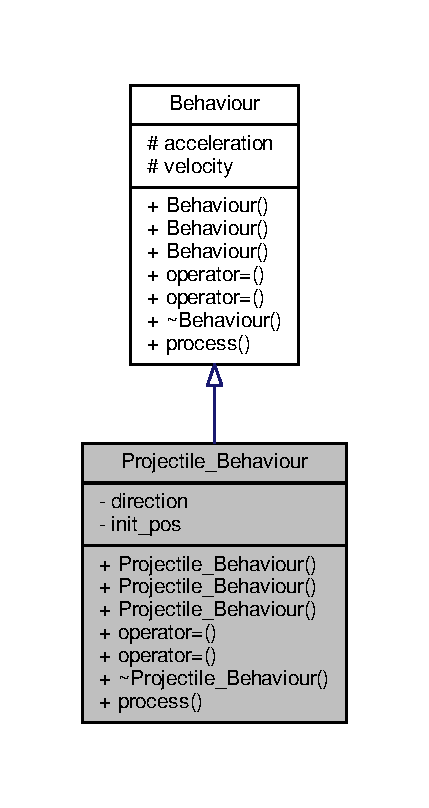
\includegraphics[width=206pt]{classProjectile__Behaviour__inherit__graph}
\end{center}
\end{figure}


Collaboration diagram for Projectile\+\_\+\+Behaviour\+:\nopagebreak
\begin{figure}[H]
\begin{center}
\leavevmode
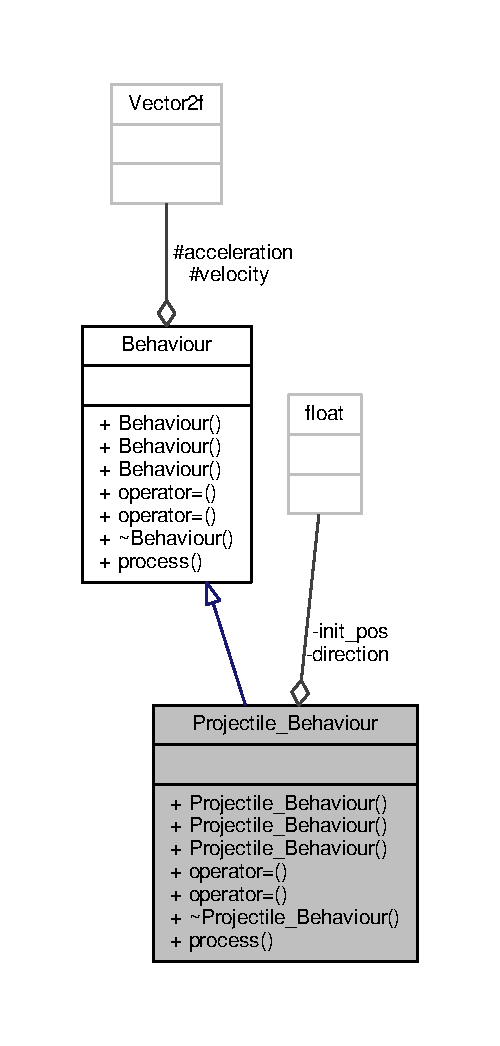
\includegraphics[width=240pt]{classProjectile__Behaviour__coll__graph}
\end{center}
\end{figure}
\subsection*{Public Member Functions}
\begin{DoxyCompactItemize}
\item 
\hyperlink{classProjectile__Behaviour_a460172a4c8d52af1dc55f1eb7f624ef1}{Projectile\+\_\+\+Behaviour} (float, float)
\item 
\hyperlink{classProjectile__Behaviour_a0c1dc1a0ad304692db0c088e51b0f19c}{Projectile\+\_\+\+Behaviour} (\hyperlink{classProjectile__Behaviour}{Projectile\+\_\+\+Behaviour} const \&other)=delete
\begin{DoxyCompactList}\small\item\em Copy konstruktor. \end{DoxyCompactList}\item 
\hyperlink{classProjectile__Behaviour_aee521a8bd5d09005746ee0e9042137de}{Projectile\+\_\+\+Behaviour} (\hyperlink{classProjectile__Behaviour}{Projectile\+\_\+\+Behaviour} \&\&other)=delete
\begin{DoxyCompactList}\small\item\em Move konstruktor. \end{DoxyCompactList}\item 
\hyperlink{classProjectile__Behaviour}{Projectile\+\_\+\+Behaviour} \& \hyperlink{classProjectile__Behaviour_ae45e301589b2c50eef8de0b9ea5e71b0}{operator=} (\hyperlink{classProjectile__Behaviour}{Projectile\+\_\+\+Behaviour} const \&rhs)\&=delete
\begin{DoxyCompactList}\small\item\em Copy operator. \end{DoxyCompactList}\item 
\hyperlink{classProjectile__Behaviour}{Projectile\+\_\+\+Behaviour} \& \hyperlink{classProjectile__Behaviour_a1e3c2f59645bec71a85d0d2689782006}{operator=} (\hyperlink{classProjectile__Behaviour}{Projectile\+\_\+\+Behaviour} \&\&rhs)=delete
\begin{DoxyCompactList}\small\item\em Move operator. \end{DoxyCompactList}\item 
\hyperlink{classProjectile__Behaviour_a162b3629a2d387c82f8f7365b0ee271e}{$\sim$\+Projectile\+\_\+\+Behaviour} ()=default
\begin{DoxyCompactList}\small\item\em Default Destruktor. \end{DoxyCompactList}\item 
void \hyperlink{classProjectile__Behaviour_aed04c8c1f5ae6aca08bdf05b6248d24a}{process} (\hyperlink{classWorld}{World} \&, \hyperlink{classEntity}{Entity} \&, sf\+::\+Time const \&) override
\begin{DoxyCompactList}\small\item\em Process som låter projektilen flyga iväg, kollidera med fiender och väggar. \end{DoxyCompactList}\end{DoxyCompactItemize}
\subsection*{Protected Attributes}
\begin{DoxyCompactItemize}
\item 
sf\+::\+Vector2f \hyperlink{classBehaviour_ac17cf81ceee6a44e8a8ec6ee810c9fd3}{acceleration} \{0.\+0f, 0.\+1f\}
\begin{DoxyCompactList}\small\item\em Variabel för gravitation. \end{DoxyCompactList}\item 
sf\+::\+Vector2f \hyperlink{classBehaviour_a1d52096cf20a59890f7705acbaccf88a}{velocity} \{0.\+0f,0.\+0f\}
\begin{DoxyCompactList}\small\item\em Variabel for hastigheten för entiteten. \end{DoxyCompactList}\end{DoxyCompactItemize}
\subsection*{Private Attributes}
\begin{DoxyCompactItemize}
\item 
float \hyperlink{classProjectile__Behaviour_a561a5badb72f1069375e4662baf8fd2d}{direction} \{\}
\begin{DoxyCompactList}\small\item\em Variabel som håller koll på vilket håll projektilen ska flyga åt. \end{DoxyCompactList}\item 
float \hyperlink{classProjectile__Behaviour_abf935a525d34c12810063c48a54d495e}{init\+\_\+pos} \{\}
\begin{DoxyCompactList}\small\item\em Variabel som sparar undan var projektilen startade ifrån. \end{DoxyCompactList}\end{DoxyCompactItemize}


\subsection{Detailed Description}
\hyperlink{classProjectile__Behaviour}{Projectile\+\_\+\+Behaviour} ärver från \hyperlink{classBehaviour}{Behaviour} och tillhandahåller beteendet för projektiler. 

\hyperlink{classProjectile__Behaviour}{Projectile\+\_\+\+Behaviour} ger projektiler deras beteende. Den gör så att projektilen åker ifrån spelaren i den riktining som spelaren tittar. Projektilen åker sedan tills den kolliderar med ett objekt som inte är en projektil eller en spelare. Den dödar objektet om det är en \hyperlink{classEnemy}{Enemy}. 

\subsection{Constructor \& Destructor Documentation}
\hypertarget{classProjectile__Behaviour_a460172a4c8d52af1dc55f1eb7f624ef1}{\index{Projectile\+\_\+\+Behaviour@{Projectile\+\_\+\+Behaviour}!Projectile\+\_\+\+Behaviour@{Projectile\+\_\+\+Behaviour}}
\index{Projectile\+\_\+\+Behaviour@{Projectile\+\_\+\+Behaviour}!Projectile\+\_\+\+Behaviour@{Projectile\+\_\+\+Behaviour}}
\subsubsection[{Projectile\+\_\+\+Behaviour}]{\setlength{\rightskip}{0pt plus 5cm}Projectile\+\_\+\+Behaviour\+::\+Projectile\+\_\+\+Behaviour (
\begin{DoxyParamCaption}
\item[{float}]{dir, }
\item[{float}]{init\+\_\+pos}
\end{DoxyParamCaption}
)}}\label{classProjectile__Behaviour_a460172a4c8d52af1dc55f1eb7f624ef1}
En konstruktor som tar emot vilket håll projektilen ska åka åt och var den startar. \hypertarget{classProjectile__Behaviour_a0c1dc1a0ad304692db0c088e51b0f19c}{\index{Projectile\+\_\+\+Behaviour@{Projectile\+\_\+\+Behaviour}!Projectile\+\_\+\+Behaviour@{Projectile\+\_\+\+Behaviour}}
\index{Projectile\+\_\+\+Behaviour@{Projectile\+\_\+\+Behaviour}!Projectile\+\_\+\+Behaviour@{Projectile\+\_\+\+Behaviour}}
\subsubsection[{Projectile\+\_\+\+Behaviour}]{\setlength{\rightskip}{0pt plus 5cm}Projectile\+\_\+\+Behaviour\+::\+Projectile\+\_\+\+Behaviour (
\begin{DoxyParamCaption}
\item[{{\bf Projectile\+\_\+\+Behaviour} const \&}]{other}
\end{DoxyParamCaption}
)\hspace{0.3cm}{\ttfamily [delete]}}}\label{classProjectile__Behaviour_a0c1dc1a0ad304692db0c088e51b0f19c}


Copy konstruktor. 

\hypertarget{classProjectile__Behaviour_aee521a8bd5d09005746ee0e9042137de}{\index{Projectile\+\_\+\+Behaviour@{Projectile\+\_\+\+Behaviour}!Projectile\+\_\+\+Behaviour@{Projectile\+\_\+\+Behaviour}}
\index{Projectile\+\_\+\+Behaviour@{Projectile\+\_\+\+Behaviour}!Projectile\+\_\+\+Behaviour@{Projectile\+\_\+\+Behaviour}}
\subsubsection[{Projectile\+\_\+\+Behaviour}]{\setlength{\rightskip}{0pt plus 5cm}Projectile\+\_\+\+Behaviour\+::\+Projectile\+\_\+\+Behaviour (
\begin{DoxyParamCaption}
\item[{{\bf Projectile\+\_\+\+Behaviour} \&\&}]{other}
\end{DoxyParamCaption}
)\hspace{0.3cm}{\ttfamily [delete]}}}\label{classProjectile__Behaviour_aee521a8bd5d09005746ee0e9042137de}


Move konstruktor. 

\hypertarget{classProjectile__Behaviour_a162b3629a2d387c82f8f7365b0ee271e}{\index{Projectile\+\_\+\+Behaviour@{Projectile\+\_\+\+Behaviour}!````~Projectile\+\_\+\+Behaviour@{$\sim$\+Projectile\+\_\+\+Behaviour}}
\index{````~Projectile\+\_\+\+Behaviour@{$\sim$\+Projectile\+\_\+\+Behaviour}!Projectile\+\_\+\+Behaviour@{Projectile\+\_\+\+Behaviour}}
\subsubsection[{$\sim$\+Projectile\+\_\+\+Behaviour}]{\setlength{\rightskip}{0pt plus 5cm}Projectile\+\_\+\+Behaviour\+::$\sim$\+Projectile\+\_\+\+Behaviour (
\begin{DoxyParamCaption}
{}
\end{DoxyParamCaption}
)\hspace{0.3cm}{\ttfamily [default]}}}\label{classProjectile__Behaviour_a162b3629a2d387c82f8f7365b0ee271e}


Default Destruktor. 



\subsection{Member Function Documentation}
\hypertarget{classProjectile__Behaviour_ae45e301589b2c50eef8de0b9ea5e71b0}{\index{Projectile\+\_\+\+Behaviour@{Projectile\+\_\+\+Behaviour}!operator=@{operator=}}
\index{operator=@{operator=}!Projectile\+\_\+\+Behaviour@{Projectile\+\_\+\+Behaviour}}
\subsubsection[{operator=}]{\setlength{\rightskip}{0pt plus 5cm}{\bf Projectile\+\_\+\+Behaviour}\& Projectile\+\_\+\+Behaviour\+::operator= (
\begin{DoxyParamCaption}
\item[{{\bf Projectile\+\_\+\+Behaviour} const \&}]{rhs}
\end{DoxyParamCaption}
)\hspace{0.3cm}{\ttfamily [delete]}}}\label{classProjectile__Behaviour_ae45e301589b2c50eef8de0b9ea5e71b0}


Copy operator. 

\hypertarget{classProjectile__Behaviour_a1e3c2f59645bec71a85d0d2689782006}{\index{Projectile\+\_\+\+Behaviour@{Projectile\+\_\+\+Behaviour}!operator=@{operator=}}
\index{operator=@{operator=}!Projectile\+\_\+\+Behaviour@{Projectile\+\_\+\+Behaviour}}
\subsubsection[{operator=}]{\setlength{\rightskip}{0pt plus 5cm}{\bf Projectile\+\_\+\+Behaviour}\& Projectile\+\_\+\+Behaviour\+::operator= (
\begin{DoxyParamCaption}
\item[{{\bf Projectile\+\_\+\+Behaviour} \&\&}]{rhs}
\end{DoxyParamCaption}
)\hspace{0.3cm}{\ttfamily [delete]}}}\label{classProjectile__Behaviour_a1e3c2f59645bec71a85d0d2689782006}


Move operator. 

\hypertarget{classProjectile__Behaviour_aed04c8c1f5ae6aca08bdf05b6248d24a}{\index{Projectile\+\_\+\+Behaviour@{Projectile\+\_\+\+Behaviour}!process@{process}}
\index{process@{process}!Projectile\+\_\+\+Behaviour@{Projectile\+\_\+\+Behaviour}}
\subsubsection[{process}]{\setlength{\rightskip}{0pt plus 5cm}void Projectile\+\_\+\+Behaviour\+::process (
\begin{DoxyParamCaption}
\item[{{\bf World} \&}]{world, }
\item[{{\bf Entity} \&}]{owner, }
\item[{sf\+::\+Time const \&}]{t}
\end{DoxyParamCaption}
)\hspace{0.3cm}{\ttfamily [override]}, {\ttfamily [virtual]}}}\label{classProjectile__Behaviour_aed04c8c1f5ae6aca08bdf05b6248d24a}


Process som låter projektilen flyga iväg, kollidera med fiender och väggar. 



Implements \hyperlink{classBehaviour_aaa6b4ee24dc3cc546fa4dbb7ba4d20da}{Behaviour}.



\subsection{Member Data Documentation}
\hypertarget{classBehaviour_ac17cf81ceee6a44e8a8ec6ee810c9fd3}{\index{Projectile\+\_\+\+Behaviour@{Projectile\+\_\+\+Behaviour}!acceleration@{acceleration}}
\index{acceleration@{acceleration}!Projectile\+\_\+\+Behaviour@{Projectile\+\_\+\+Behaviour}}
\subsubsection[{acceleration}]{\setlength{\rightskip}{0pt plus 5cm}sf\+::\+Vector2f Behaviour\+::acceleration \{0.\+0f, 0.\+1f\}\hspace{0.3cm}{\ttfamily [protected]}, {\ttfamily [inherited]}}}\label{classBehaviour_ac17cf81ceee6a44e8a8ec6ee810c9fd3}


Variabel för gravitation. 

\hypertarget{classProjectile__Behaviour_a561a5badb72f1069375e4662baf8fd2d}{\index{Projectile\+\_\+\+Behaviour@{Projectile\+\_\+\+Behaviour}!direction@{direction}}
\index{direction@{direction}!Projectile\+\_\+\+Behaviour@{Projectile\+\_\+\+Behaviour}}
\subsubsection[{direction}]{\setlength{\rightskip}{0pt plus 5cm}float Projectile\+\_\+\+Behaviour\+::direction \{\}\hspace{0.3cm}{\ttfamily [private]}}}\label{classProjectile__Behaviour_a561a5badb72f1069375e4662baf8fd2d}


Variabel som håller koll på vilket håll projektilen ska flyga åt. 

\hypertarget{classProjectile__Behaviour_abf935a525d34c12810063c48a54d495e}{\index{Projectile\+\_\+\+Behaviour@{Projectile\+\_\+\+Behaviour}!init\+\_\+pos@{init\+\_\+pos}}
\index{init\+\_\+pos@{init\+\_\+pos}!Projectile\+\_\+\+Behaviour@{Projectile\+\_\+\+Behaviour}}
\subsubsection[{init\+\_\+pos}]{\setlength{\rightskip}{0pt plus 5cm}float Projectile\+\_\+\+Behaviour\+::init\+\_\+pos \{\}\hspace{0.3cm}{\ttfamily [private]}}}\label{classProjectile__Behaviour_abf935a525d34c12810063c48a54d495e}


Variabel som sparar undan var projektilen startade ifrån. 

\hypertarget{classBehaviour_a1d52096cf20a59890f7705acbaccf88a}{\index{Projectile\+\_\+\+Behaviour@{Projectile\+\_\+\+Behaviour}!velocity@{velocity}}
\index{velocity@{velocity}!Projectile\+\_\+\+Behaviour@{Projectile\+\_\+\+Behaviour}}
\subsubsection[{velocity}]{\setlength{\rightskip}{0pt plus 5cm}sf\+::\+Vector2f Behaviour\+::velocity \{0.\+0f,0.\+0f\}\hspace{0.3cm}{\ttfamily [protected]}, {\ttfamily [inherited]}}}\label{classBehaviour_a1d52096cf20a59890f7705acbaccf88a}


Variabel for hastigheten för entiteten. 



The documentation for this class was generated from the following files\+:\begin{DoxyCompactItemize}
\item 
source/objects/headers/Projectile\+\_\+\+Behaviour.\+h\item 
source/objects/imps/Projectile\+\_\+\+Behaviour.\+cpp\end{DoxyCompactItemize}

\hypertarget{classTexture__Container}{\section{Texture\+\_\+\+Container Class Reference}
\label{classTexture__Container}\index{Texture\+\_\+\+Container@{Texture\+\_\+\+Container}}
}


\hyperlink{classTexture__Container}{Texture\+\_\+\+Container} tillhandahåller texturer till alla entiteter.  




{\ttfamily \#include $<$Texture\+\_\+\+Container.\+h$>$}



Collaboration diagram for Texture\+\_\+\+Container\+:\nopagebreak
\begin{figure}[H]
\begin{center}
\leavevmode
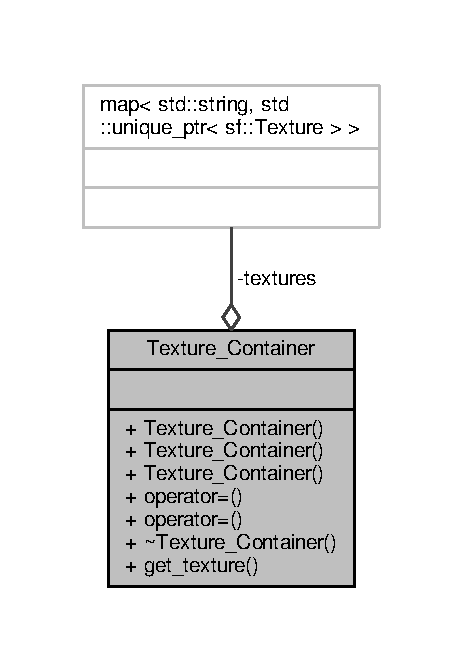
\includegraphics[width=222pt]{classTexture__Container__coll__graph}
\end{center}
\end{figure}
\subsection*{Public Member Functions}
\begin{DoxyCompactItemize}
\item 
\hyperlink{classTexture__Container_a40fff5e61bf994ba704a43e87b3e3a18}{Texture\+\_\+\+Container} ()
\begin{DoxyCompactList}\small\item\em Vanlig Konstruktor. \end{DoxyCompactList}\item 
\hyperlink{classTexture__Container_aa5bb29d2e6f49cf6e9784d18888d95e5}{Texture\+\_\+\+Container} (\hyperlink{classTexture__Container}{Texture\+\_\+\+Container} const \&other)=delete
\begin{DoxyCompactList}\small\item\em Copy konstruktor. \end{DoxyCompactList}\item 
\hyperlink{classTexture__Container_a372127d3c359f96c7c4aa3b2106e3fd7}{Texture\+\_\+\+Container} (\hyperlink{classTexture__Container}{Texture\+\_\+\+Container} \&\&other)=delete
\begin{DoxyCompactList}\small\item\em Move konstruktor. \end{DoxyCompactList}\item 
\hyperlink{classTexture__Container}{Texture\+\_\+\+Container} \& \hyperlink{classTexture__Container_aaf58055affd862bac102efebfeb41bbc}{operator=} (\hyperlink{classTexture__Container}{Texture\+\_\+\+Container} const \&rhs)\&=delete
\begin{DoxyCompactList}\small\item\em Copy operator. \end{DoxyCompactList}\item 
\hyperlink{classTexture__Container}{Texture\+\_\+\+Container} \& \hyperlink{classTexture__Container_a9364b90bbf24d4b582c868e37de2e1ec}{operator=} (\hyperlink{classTexture__Container}{Texture\+\_\+\+Container} \&\&rhs)=delete
\begin{DoxyCompactList}\small\item\em Move operator. \end{DoxyCompactList}\item 
\hyperlink{classTexture__Container_a8b07cb110e4d35f2c4b42c67ab4ddda0}{$\sim$\+Texture\+\_\+\+Container} ()=default
\begin{DoxyCompactList}\small\item\em Default Destruktor. \end{DoxyCompactList}\item 
sf\+::\+Texture const \& \hyperlink{classTexture__Container_afce993abd37ca2a9647a154a561a6e74}{get\+\_\+texture} (std\+::string) const 
\begin{DoxyCompactList}\small\item\em En funktion som returnerar den textur som har namnet strängen anger. \end{DoxyCompactList}\end{DoxyCompactItemize}
\subsection*{Private Attributes}
\begin{DoxyCompactItemize}
\item 
std\+::map$<$ std\+::string, \\*
std\+::unique\+\_\+ptr$<$ sf\+::\+Texture $>$ $>$ \hyperlink{classTexture__Container_a2adf8e4fde3c21db9c92d99c77b1116a}{textures}
\begin{DoxyCompactList}\small\item\em En std\+::map som innehåller unika smart pekare. \end{DoxyCompactList}\end{DoxyCompactItemize}


\subsection{Detailed Description}
\hyperlink{classTexture__Container}{Texture\+\_\+\+Container} tillhandahåller texturer till alla entiteter. 

\hyperlink{classTexture__Container}{Texture\+\_\+\+Container} läser in alla grafiska bitar av spelet och tillhandahåller pekare till dessa. Detta för att använda mindre grafiskt minne. 

\subsection{Constructor \& Destructor Documentation}
\hypertarget{classTexture__Container_a40fff5e61bf994ba704a43e87b3e3a18}{\index{Texture\+\_\+\+Container@{Texture\+\_\+\+Container}!Texture\+\_\+\+Container@{Texture\+\_\+\+Container}}
\index{Texture\+\_\+\+Container@{Texture\+\_\+\+Container}!Texture\+\_\+\+Container@{Texture\+\_\+\+Container}}
\subsubsection[{Texture\+\_\+\+Container}]{\setlength{\rightskip}{0pt plus 5cm}Texture\+\_\+\+Container\+::\+Texture\+\_\+\+Container (
\begin{DoxyParamCaption}
{}
\end{DoxyParamCaption}
)}}\label{classTexture__Container_a40fff5e61bf994ba704a43e87b3e3a18}


Vanlig Konstruktor. 

\hypertarget{classTexture__Container_aa5bb29d2e6f49cf6e9784d18888d95e5}{\index{Texture\+\_\+\+Container@{Texture\+\_\+\+Container}!Texture\+\_\+\+Container@{Texture\+\_\+\+Container}}
\index{Texture\+\_\+\+Container@{Texture\+\_\+\+Container}!Texture\+\_\+\+Container@{Texture\+\_\+\+Container}}
\subsubsection[{Texture\+\_\+\+Container}]{\setlength{\rightskip}{0pt plus 5cm}Texture\+\_\+\+Container\+::\+Texture\+\_\+\+Container (
\begin{DoxyParamCaption}
\item[{{\bf Texture\+\_\+\+Container} const \&}]{other}
\end{DoxyParamCaption}
)\hspace{0.3cm}{\ttfamily [delete]}}}\label{classTexture__Container_aa5bb29d2e6f49cf6e9784d18888d95e5}


Copy konstruktor. 

\hypertarget{classTexture__Container_a372127d3c359f96c7c4aa3b2106e3fd7}{\index{Texture\+\_\+\+Container@{Texture\+\_\+\+Container}!Texture\+\_\+\+Container@{Texture\+\_\+\+Container}}
\index{Texture\+\_\+\+Container@{Texture\+\_\+\+Container}!Texture\+\_\+\+Container@{Texture\+\_\+\+Container}}
\subsubsection[{Texture\+\_\+\+Container}]{\setlength{\rightskip}{0pt plus 5cm}Texture\+\_\+\+Container\+::\+Texture\+\_\+\+Container (
\begin{DoxyParamCaption}
\item[{{\bf Texture\+\_\+\+Container} \&\&}]{other}
\end{DoxyParamCaption}
)\hspace{0.3cm}{\ttfamily [delete]}}}\label{classTexture__Container_a372127d3c359f96c7c4aa3b2106e3fd7}


Move konstruktor. 

\hypertarget{classTexture__Container_a8b07cb110e4d35f2c4b42c67ab4ddda0}{\index{Texture\+\_\+\+Container@{Texture\+\_\+\+Container}!````~Texture\+\_\+\+Container@{$\sim$\+Texture\+\_\+\+Container}}
\index{````~Texture\+\_\+\+Container@{$\sim$\+Texture\+\_\+\+Container}!Texture\+\_\+\+Container@{Texture\+\_\+\+Container}}
\subsubsection[{$\sim$\+Texture\+\_\+\+Container}]{\setlength{\rightskip}{0pt plus 5cm}Texture\+\_\+\+Container\+::$\sim$\+Texture\+\_\+\+Container (
\begin{DoxyParamCaption}
{}
\end{DoxyParamCaption}
)\hspace{0.3cm}{\ttfamily [default]}}}\label{classTexture__Container_a8b07cb110e4d35f2c4b42c67ab4ddda0}


Default Destruktor. 



\subsection{Member Function Documentation}
\hypertarget{classTexture__Container_afce993abd37ca2a9647a154a561a6e74}{\index{Texture\+\_\+\+Container@{Texture\+\_\+\+Container}!get\+\_\+texture@{get\+\_\+texture}}
\index{get\+\_\+texture@{get\+\_\+texture}!Texture\+\_\+\+Container@{Texture\+\_\+\+Container}}
\subsubsection[{get\+\_\+texture}]{\setlength{\rightskip}{0pt plus 5cm}sf\+::\+Texture const \& Texture\+\_\+\+Container\+::get\+\_\+texture (
\begin{DoxyParamCaption}
\item[{std\+::string}]{name}
\end{DoxyParamCaption}
) const}}\label{classTexture__Container_afce993abd37ca2a9647a154a561a6e74}


En funktion som returnerar den textur som har namnet strängen anger. 

\hypertarget{classTexture__Container_aaf58055affd862bac102efebfeb41bbc}{\index{Texture\+\_\+\+Container@{Texture\+\_\+\+Container}!operator=@{operator=}}
\index{operator=@{operator=}!Texture\+\_\+\+Container@{Texture\+\_\+\+Container}}
\subsubsection[{operator=}]{\setlength{\rightskip}{0pt plus 5cm}{\bf Texture\+\_\+\+Container}\& Texture\+\_\+\+Container\+::operator= (
\begin{DoxyParamCaption}
\item[{{\bf Texture\+\_\+\+Container} const \&}]{rhs}
\end{DoxyParamCaption}
)\hspace{0.3cm}{\ttfamily [delete]}}}\label{classTexture__Container_aaf58055affd862bac102efebfeb41bbc}


Copy operator. 

\hypertarget{classTexture__Container_a9364b90bbf24d4b582c868e37de2e1ec}{\index{Texture\+\_\+\+Container@{Texture\+\_\+\+Container}!operator=@{operator=}}
\index{operator=@{operator=}!Texture\+\_\+\+Container@{Texture\+\_\+\+Container}}
\subsubsection[{operator=}]{\setlength{\rightskip}{0pt plus 5cm}{\bf Texture\+\_\+\+Container}\& Texture\+\_\+\+Container\+::operator= (
\begin{DoxyParamCaption}
\item[{{\bf Texture\+\_\+\+Container} \&\&}]{rhs}
\end{DoxyParamCaption}
)\hspace{0.3cm}{\ttfamily [delete]}}}\label{classTexture__Container_a9364b90bbf24d4b582c868e37de2e1ec}


Move operator. 



\subsection{Member Data Documentation}
\hypertarget{classTexture__Container_a2adf8e4fde3c21db9c92d99c77b1116a}{\index{Texture\+\_\+\+Container@{Texture\+\_\+\+Container}!textures@{textures}}
\index{textures@{textures}!Texture\+\_\+\+Container@{Texture\+\_\+\+Container}}
\subsubsection[{textures}]{\setlength{\rightskip}{0pt plus 5cm}std\+::map$<$std\+::string, std\+::unique\+\_\+ptr$<$sf\+::\+Texture$>$ $>$ Texture\+\_\+\+Container\+::textures\hspace{0.3cm}{\ttfamily [private]}}}\label{classTexture__Container_a2adf8e4fde3c21db9c92d99c77b1116a}


En std\+::map som innehåller unika smart pekare. 



The documentation for this class was generated from the following files\+:\begin{DoxyCompactItemize}
\item 
source/objects/headers/Texture\+\_\+\+Container.\+h\item 
source/objects/imps/Texture\+\_\+\+Container.\+cpp\end{DoxyCompactItemize}

\hypertarget{classWorld}{\section{World Class Reference}
\label{classWorld}\index{World@{World}}
}


\hyperlink{classWorld}{World} simulerar spelvärlden.  




{\ttfamily \#include $<$World.\+h$>$}



Collaboration diagram for World\+:\nopagebreak
\begin{figure}[H]
\begin{center}
\leavevmode
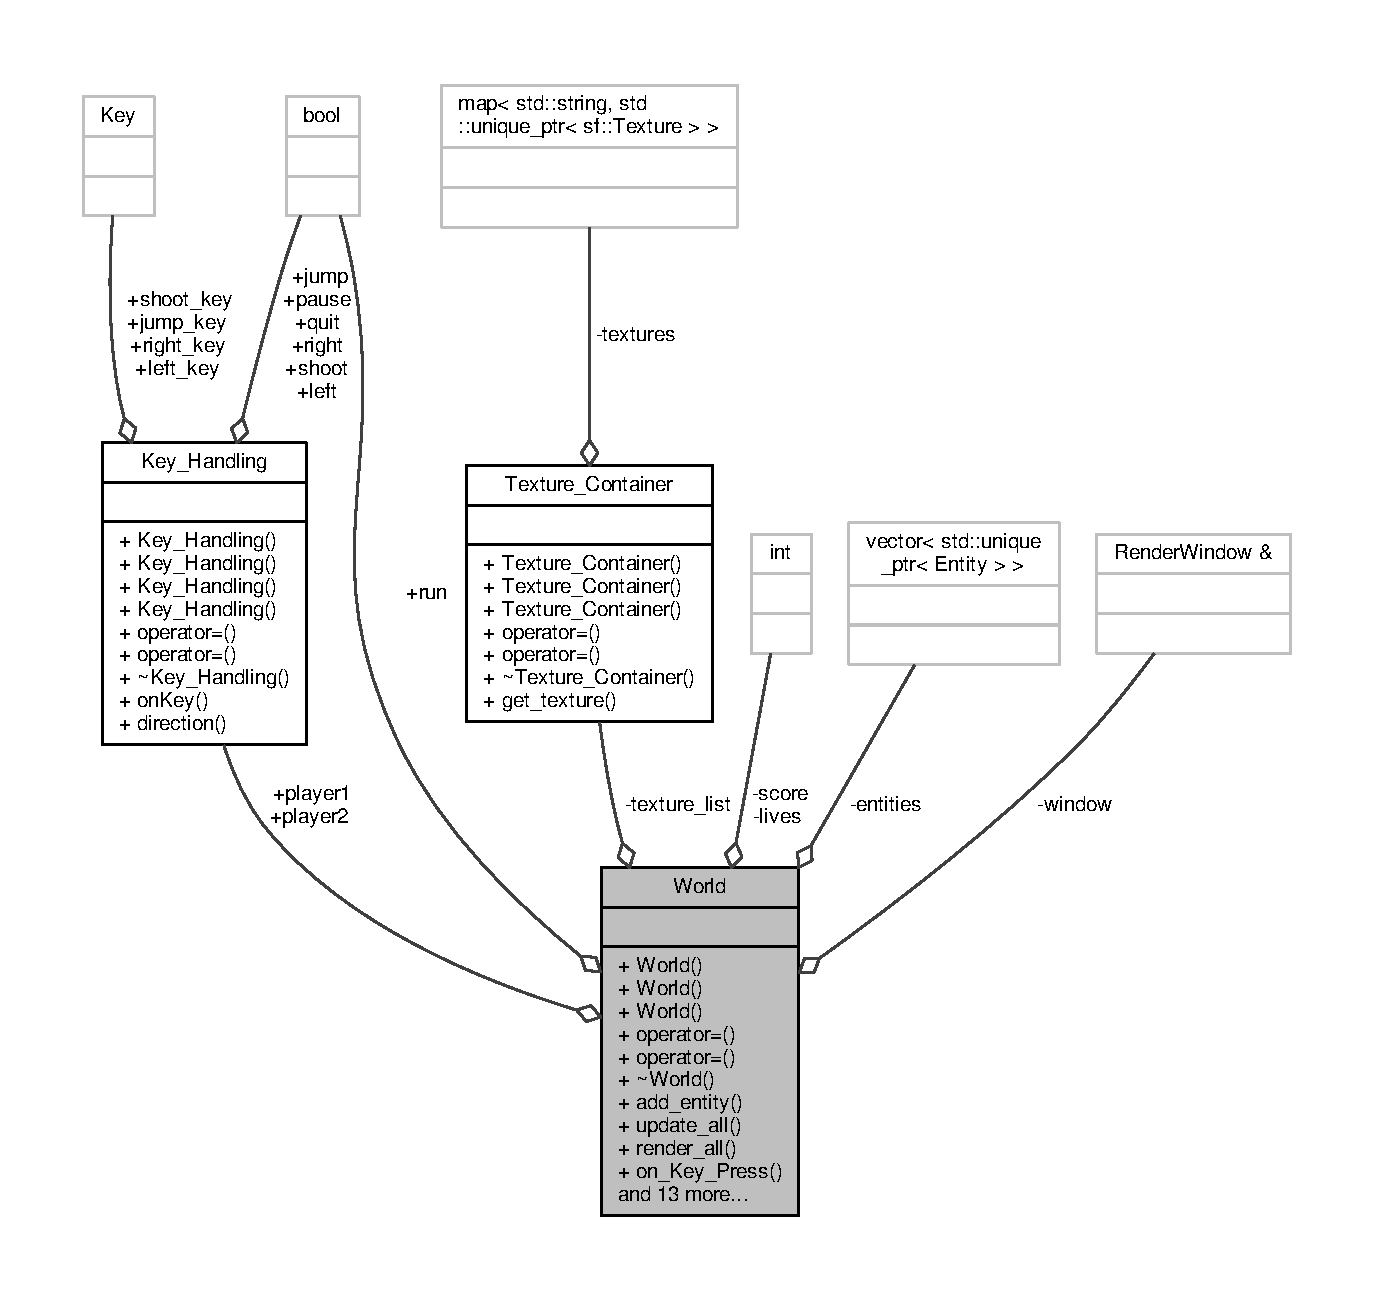
\includegraphics[width=350pt]{classWorld__coll__graph}
\end{center}
\end{figure}
\subsection*{Public Member Functions}
\begin{DoxyCompactItemize}
\item 
\hyperlink{classWorld_a64c31c6063dddddaa69ff078fcfaac3f}{World} (sf\+::\+Render\+Window \&)
\begin{DoxyCompactList}\small\item\em \hyperlink{classWorld}{World}'s konstruktor tar in ett sf\+::\+Render\+Window och sparar detta i en variabel. \end{DoxyCompactList}\item 
\hyperlink{classWorld_a69eeaec5442964e520c638fbbba5ad29}{World} (\hyperlink{classWorld}{World} const \&other)=delete
\begin{DoxyCompactList}\small\item\em Copy konstruktor. \end{DoxyCompactList}\item 
\hyperlink{classWorld_a9319f9fe52db6162be2269479d76100d}{World} (\hyperlink{classWorld}{World} \&\&other)=delete
\begin{DoxyCompactList}\small\item\em Move konstruktor. \end{DoxyCompactList}\item 
\hyperlink{classWorld}{World} \& \hyperlink{classWorld_a93bf098ff19ca834e40b011a03a25ed8}{operator=} (\hyperlink{classWorld}{World} const \&rhs)\&=delete
\begin{DoxyCompactList}\small\item\em Copy operator. \end{DoxyCompactList}\item 
\hyperlink{classWorld}{World} \& \hyperlink{classWorld_a81066ed30db54ae9060f9394d6f2c01e}{operator=} (\hyperlink{classWorld}{World} \&\&rhs)=delete
\begin{DoxyCompactList}\small\item\em Move operator. \end{DoxyCompactList}\item 
\hyperlink{classWorld_a3d07ed2f713c3946fbbaa3a1b7b7f8c0}{$\sim$\+World} ()=default
\begin{DoxyCompactList}\small\item\em Default destruktor. \end{DoxyCompactList}\item 
void \hyperlink{classWorld_ae6af4b63e388f6dde1ccaa5afe2592be}{add\+\_\+entity} (\hyperlink{classEntity}{Entity} $\ast$)
\item 
void \hyperlink{classWorld_abe8efb7955edd02cfdae5f99f2e5a346}{update\+\_\+all} (sf\+::\+Time const \&)
\begin{DoxyCompactList}\small\item\em Går igenom World\+::\+Entities och kör deras Entity\+::\+Update(). \end{DoxyCompactList}\item 
void \hyperlink{classWorld_a56d3640e46fef8b3e62538f067e2fbd2}{render\+\_\+all} () const 
\begin{DoxyCompactList}\small\item\em Går igenom World\+::\+Entities och ritar dessa till window. \end{DoxyCompactList}\item 
void \hyperlink{classWorld_adfa428160c22b1e420048bdcacc93733}{on\+\_\+\+Key\+\_\+\+Press} (sf\+::\+Keyboard\+::\+Key)
\begin{DoxyCompactList}\small\item\em Tar hand om tangenttryckningar genom att skicka true när den trycks ner. \end{DoxyCompactList}\item 
void \hyperlink{classWorld_a2162e66648702260f49e0bece2ea67df}{on\+\_\+\+Key\+\_\+\+Release} (sf\+::\+Keyboard\+::\+Key)
\begin{DoxyCompactList}\small\item\em Tar hand om tangenttryckningar genom att skicka false när den släpps upp. \end{DoxyCompactList}\item 
\hyperlink{classEntity}{Entity} $\ast$ \hyperlink{classWorld_a6f3662fed56503455d176e85c2e45292}{am\+\_\+\+I\+\_\+\+Colliding} (\hyperlink{classEntity}{Entity} const \&) const 
\item 
void \hyperlink{classWorld_aba7ebab445704a4db31e9407e894cb3e}{kill\+\_\+me\+\_\+now} (\hyperlink{classEntity}{Entity} \&)
\item 
\hyperlink{classEntity}{Entity} $\ast$ \hyperlink{classWorld_a0b4bf20ce8e70ec398fb40d6366cb222}{get\+\_\+player} () const 
\item 
void \hyperlink{classWorld_a24f6906f2e4f0c761653a8f9e42588a6}{clear} ()
\item 
bool \hyperlink{classWorld_afe79848202c75c3b9e86fc336ba60a2d}{win} () const 
\begin{DoxyCompactList}\small\item\em Om spelaren har dödat alla enemy objekt så returnerar denna true. \end{DoxyCompactList}\item 
int \hyperlink{classWorld_a6500dacbd84084f8ac056eaf04aa603b}{get\+\_\+lives} () const 
\begin{DoxyCompactList}\small\item\em Getter för \hyperlink{classWorld_af7d5c3e3405e2efaadf6cd76745440c6}{World\+::lives}. \end{DoxyCompactList}\item 
void \hyperlink{classWorld_ac7b43593b36fb380c433eddd3d075613}{add\+\_\+life} ()
\begin{DoxyCompactList}\small\item\em Lägger till 1 life. \end{DoxyCompactList}\item 
void \hyperlink{classWorld_aef42373ac6cd2f6bdacc22b7c1b14055}{remove\+\_\+life} ()
\begin{DoxyCompactList}\small\item\em Tar bort 1 life. \end{DoxyCompactList}\item 
unsigned int \hyperlink{classWorld_a999f330b74ecf28c164dcaf71423cbcb}{get\+\_\+score} () const 
\begin{DoxyCompactList}\small\item\em Getter för \hyperlink{classWorld_a8e0d399d947596356b65e8bcb5d4cad8}{World\+::score}. \end{DoxyCompactList}\item 
void \hyperlink{classWorld_ac5c27ebafb5832cd2aeac24afda475f6}{add\+\_\+score} (unsigned int)
\begin{DoxyCompactList}\small\item\em Lägger till n på score. \end{DoxyCompactList}\item 
void \hyperlink{classWorld_a697e8f216b1fa06d1b708e7847662d3a}{remove\+\_\+score} (unsigned int)
\begin{DoxyCompactList}\small\item\em tar bort n på score. \end{DoxyCompactList}\item 
sf\+::\+Texture const \& \hyperlink{classWorld_a5c35a088979ebddf7365eb3707400d2e}{get\+\_\+texture} (std\+::string name) const 
\begin{DoxyCompactList}\small\item\em Hämtar en texture från \hyperlink{classWorld_a77cc00620c137bb0b8b2620912b4dddc}{World\+::texture\+\_\+list}. \end{DoxyCompactList}\end{DoxyCompactItemize}
\subsection*{Public Attributes}
\begin{DoxyCompactItemize}
\item 
\hyperlink{classKey__Handling}{Key\+\_\+\+Handling} \hyperlink{classWorld_a9607cd0034a5a2b9638598c64d03091e}{player1}
\begin{DoxyCompactList}\small\item\em Tangent hanterare för spelare 1. \end{DoxyCompactList}\item 
\hyperlink{classKey__Handling}{Key\+\_\+\+Handling} \hyperlink{classWorld_acbb895c03359b30548afdceeba0903e6}{player2}
\begin{DoxyCompactList}\small\item\em Tangent hanterare för spelare 2. \end{DoxyCompactList}\item 
bool \hyperlink{classWorld_a3bc8666629d71e77057927b14687407b}{run} \{true\}
\begin{DoxyCompactList}\small\item\em Bool som används för att avsluta spelet. \end{DoxyCompactList}\end{DoxyCompactItemize}
\subsection*{Private Attributes}
\begin{DoxyCompactItemize}
\item 
sf\+::\+Render\+Window \& \hyperlink{classWorld_a81c4b706c899cd5cf8598ed79a691934}{window}
\begin{DoxyCompactList}\small\item\em Fönstret som illustrerar spelet. \end{DoxyCompactList}\item 
std\+::vector$<$ std\+::unique\+\_\+ptr\\*
$<$ \hyperlink{classEntity}{Entity} $>$ $>$ \hyperlink{classWorld_a74d706a3a47afe52b70f5e2dd3bf612b}{entities}
\begin{DoxyCompactList}\small\item\em En vektor av unika smart pekare som innehåller alla Entitys i världen. \end{DoxyCompactList}\item 
int \hyperlink{classWorld_af7d5c3e3405e2efaadf6cd76745440c6}{lives} \{3\}
\begin{DoxyCompactList}\small\item\em Antal liv för spelarna. \end{DoxyCompactList}\item 
unsigned int \hyperlink{classWorld_a8e0d399d947596356b65e8bcb5d4cad8}{score} \{0\}
\begin{DoxyCompactList}\small\item\em Spelarnas poäng. \end{DoxyCompactList}\item 
\hyperlink{classTexture__Container}{Texture\+\_\+\+Container} \hyperlink{classWorld_a77cc00620c137bb0b8b2620912b4dddc}{texture\+\_\+list} \{\}
\begin{DoxyCompactList}\small\item\em En \hyperlink{classTexture__Container}{Texture\+\_\+\+Container} som innehåller alla grafiska delar av spelet. \end{DoxyCompactList}\end{DoxyCompactItemize}


\subsection{Detailed Description}
\hyperlink{classWorld}{World} simulerar spelvärlden. 

\hyperlink{classWorld}{World} utför simulation av spelvärlden. Den baserar sig på S\+F\+M\+Ls inbyggda positions system och uppdaterar entiteter varje gång \hyperlink{classWorld_abe8efb7955edd02cfdae5f99f2e5a346}{update\+\_\+all()} kallas på. Klassen håller också koll på input från användaren, hur många extraliv en spelare har och hur många poäng denne har. 

\subsection{Constructor \& Destructor Documentation}
\hypertarget{classWorld_a64c31c6063dddddaa69ff078fcfaac3f}{\index{World@{World}!World@{World}}
\index{World@{World}!World@{World}}
\subsubsection[{World}]{\setlength{\rightskip}{0pt plus 5cm}World\+::\+World (
\begin{DoxyParamCaption}
\item[{sf\+::\+Render\+Window \&}]{w}
\end{DoxyParamCaption}
)}}\label{classWorld_a64c31c6063dddddaa69ff078fcfaac3f}


\hyperlink{classWorld}{World}'s konstruktor tar in ett sf\+::\+Render\+Window och sparar detta i en variabel. 

\hypertarget{classWorld_a69eeaec5442964e520c638fbbba5ad29}{\index{World@{World}!World@{World}}
\index{World@{World}!World@{World}}
\subsubsection[{World}]{\setlength{\rightskip}{0pt plus 5cm}World\+::\+World (
\begin{DoxyParamCaption}
\item[{{\bf World} const \&}]{other}
\end{DoxyParamCaption}
)\hspace{0.3cm}{\ttfamily [delete]}}}\label{classWorld_a69eeaec5442964e520c638fbbba5ad29}


Copy konstruktor. 

\hypertarget{classWorld_a9319f9fe52db6162be2269479d76100d}{\index{World@{World}!World@{World}}
\index{World@{World}!World@{World}}
\subsubsection[{World}]{\setlength{\rightskip}{0pt plus 5cm}World\+::\+World (
\begin{DoxyParamCaption}
\item[{{\bf World} \&\&}]{other}
\end{DoxyParamCaption}
)\hspace{0.3cm}{\ttfamily [delete]}}}\label{classWorld_a9319f9fe52db6162be2269479d76100d}


Move konstruktor. 

\hypertarget{classWorld_a3d07ed2f713c3946fbbaa3a1b7b7f8c0}{\index{World@{World}!````~World@{$\sim$\+World}}
\index{````~World@{$\sim$\+World}!World@{World}}
\subsubsection[{$\sim$\+World}]{\setlength{\rightskip}{0pt plus 5cm}World\+::$\sim$\+World (
\begin{DoxyParamCaption}
{}
\end{DoxyParamCaption}
)\hspace{0.3cm}{\ttfamily [default]}}}\label{classWorld_a3d07ed2f713c3946fbbaa3a1b7b7f8c0}


Default destruktor. 



\subsection{Member Function Documentation}
\hypertarget{classWorld_ae6af4b63e388f6dde1ccaa5afe2592be}{\index{World@{World}!add\+\_\+entity@{add\+\_\+entity}}
\index{add\+\_\+entity@{add\+\_\+entity}!World@{World}}
\subsubsection[{add\+\_\+entity}]{\setlength{\rightskip}{0pt plus 5cm}void World\+::add\+\_\+entity (
\begin{DoxyParamCaption}
\item[{{\bf Entity} $\ast$}]{e}
\end{DoxyParamCaption}
)}}\label{classWorld_ae6af4b63e388f6dde1ccaa5afe2592be}
Lägger till en \hyperlink{classEntity}{Entity} objekt pekare i World\+::\+Entities. Använder unika smart pekare för att undvika memory leaks. \hypertarget{classWorld_ac7b43593b36fb380c433eddd3d075613}{\index{World@{World}!add\+\_\+life@{add\+\_\+life}}
\index{add\+\_\+life@{add\+\_\+life}!World@{World}}
\subsubsection[{add\+\_\+life}]{\setlength{\rightskip}{0pt plus 5cm}void World\+::add\+\_\+life (
\begin{DoxyParamCaption}
{}
\end{DoxyParamCaption}
)}}\label{classWorld_ac7b43593b36fb380c433eddd3d075613}


Lägger till 1 life. 

\hypertarget{classWorld_ac5c27ebafb5832cd2aeac24afda475f6}{\index{World@{World}!add\+\_\+score@{add\+\_\+score}}
\index{add\+\_\+score@{add\+\_\+score}!World@{World}}
\subsubsection[{add\+\_\+score}]{\setlength{\rightskip}{0pt plus 5cm}void World\+::add\+\_\+score (
\begin{DoxyParamCaption}
\item[{unsigned int}]{i}
\end{DoxyParamCaption}
)}}\label{classWorld_ac5c27ebafb5832cd2aeac24afda475f6}


Lägger till n på score. 

\hypertarget{classWorld_a6f3662fed56503455d176e85c2e45292}{\index{World@{World}!am\+\_\+\+I\+\_\+\+Colliding@{am\+\_\+\+I\+\_\+\+Colliding}}
\index{am\+\_\+\+I\+\_\+\+Colliding@{am\+\_\+\+I\+\_\+\+Colliding}!World@{World}}
\subsubsection[{am\+\_\+\+I\+\_\+\+Colliding}]{\setlength{\rightskip}{0pt plus 5cm}{\bf Entity} $\ast$ World\+::am\+\_\+\+I\+\_\+\+Colliding (
\begin{DoxyParamCaption}
\item[{{\bf Entity} const \&}]{e}
\end{DoxyParamCaption}
) const}}\label{classWorld_a6f3662fed56503455d176e85c2e45292}
En funktion som returnerar ett referens till ett \hyperlink{classEntity}{Entity} objekt om det kolliderar med det objekt som tillhandahålls. Den kollar detta med hjälp av S\+F\+M\+Ls egna intersect(). Dock returnerar den bara det första objektet som kolliderar. Detta kan skapa problem. \hypertarget{classWorld_a24f6906f2e4f0c761653a8f9e42588a6}{\index{World@{World}!clear@{clear}}
\index{clear@{clear}!World@{World}}
\subsubsection[{clear}]{\setlength{\rightskip}{0pt plus 5cm}void World\+::clear (
\begin{DoxyParamCaption}
{}
\end{DoxyParamCaption}
)}}\label{classWorld_a24f6906f2e4f0c761653a8f9e42588a6}
Tar bort alla objekt i World\+::\+Entities. Detta används för att kunna skapa nya nivåer utan att de gamla stör. \hypertarget{classWorld_a6500dacbd84084f8ac056eaf04aa603b}{\index{World@{World}!get\+\_\+lives@{get\+\_\+lives}}
\index{get\+\_\+lives@{get\+\_\+lives}!World@{World}}
\subsubsection[{get\+\_\+lives}]{\setlength{\rightskip}{0pt plus 5cm}int World\+::get\+\_\+lives (
\begin{DoxyParamCaption}
{}
\end{DoxyParamCaption}
) const}}\label{classWorld_a6500dacbd84084f8ac056eaf04aa603b}


Getter för \hyperlink{classWorld_af7d5c3e3405e2efaadf6cd76745440c6}{World\+::lives}. 

\hypertarget{classWorld_a0b4bf20ce8e70ec398fb40d6366cb222}{\index{World@{World}!get\+\_\+player@{get\+\_\+player}}
\index{get\+\_\+player@{get\+\_\+player}!World@{World}}
\subsubsection[{get\+\_\+player}]{\setlength{\rightskip}{0pt plus 5cm}{\bf Entity} $\ast$ World\+::get\+\_\+player (
\begin{DoxyParamCaption}
{}
\end{DoxyParamCaption}
) const}}\label{classWorld_a0b4bf20ce8e70ec398fb40d6366cb222}
Returnerar den första spelaren i World\+::\+Entities. Används för att avgöra huruvida alla spelare har dött. \hypertarget{classWorld_a999f330b74ecf28c164dcaf71423cbcb}{\index{World@{World}!get\+\_\+score@{get\+\_\+score}}
\index{get\+\_\+score@{get\+\_\+score}!World@{World}}
\subsubsection[{get\+\_\+score}]{\setlength{\rightskip}{0pt plus 5cm}unsigned int World\+::get\+\_\+score (
\begin{DoxyParamCaption}
{}
\end{DoxyParamCaption}
) const}}\label{classWorld_a999f330b74ecf28c164dcaf71423cbcb}


Getter för \hyperlink{classWorld_a8e0d399d947596356b65e8bcb5d4cad8}{World\+::score}. 

\hypertarget{classWorld_a5c35a088979ebddf7365eb3707400d2e}{\index{World@{World}!get\+\_\+texture@{get\+\_\+texture}}
\index{get\+\_\+texture@{get\+\_\+texture}!World@{World}}
\subsubsection[{get\+\_\+texture}]{\setlength{\rightskip}{0pt plus 5cm}sf\+::\+Texture const\& World\+::get\+\_\+texture (
\begin{DoxyParamCaption}
\item[{std\+::string}]{name}
\end{DoxyParamCaption}
) const\hspace{0.3cm}{\ttfamily [inline]}}}\label{classWorld_a5c35a088979ebddf7365eb3707400d2e}


Hämtar en texture från \hyperlink{classWorld_a77cc00620c137bb0b8b2620912b4dddc}{World\+::texture\+\_\+list}. 

\hypertarget{classWorld_aba7ebab445704a4db31e9407e894cb3e}{\index{World@{World}!kill\+\_\+me\+\_\+now@{kill\+\_\+me\+\_\+now}}
\index{kill\+\_\+me\+\_\+now@{kill\+\_\+me\+\_\+now}!World@{World}}
\subsubsection[{kill\+\_\+me\+\_\+now}]{\setlength{\rightskip}{0pt plus 5cm}void World\+::kill\+\_\+me\+\_\+now (
\begin{DoxyParamCaption}
\item[{{\bf Entity} \&}]{e}
\end{DoxyParamCaption}
)}}\label{classWorld_aba7ebab445704a4db31e9407e894cb3e}
Tar bort det objekt som tillhandahålls från World\+::\+Entities. Detta genom att gå igenom och hitta den pekare i World\+::\+Entities som pekar på samma minnesaddress som objektet som tillhandahålls. Sedan tas den bort. \hypertarget{classWorld_adfa428160c22b1e420048bdcacc93733}{\index{World@{World}!on\+\_\+\+Key\+\_\+\+Press@{on\+\_\+\+Key\+\_\+\+Press}}
\index{on\+\_\+\+Key\+\_\+\+Press@{on\+\_\+\+Key\+\_\+\+Press}!World@{World}}
\subsubsection[{on\+\_\+\+Key\+\_\+\+Press}]{\setlength{\rightskip}{0pt plus 5cm}void World\+::on\+\_\+\+Key\+\_\+\+Press (
\begin{DoxyParamCaption}
\item[{sf\+::\+Keyboard\+::\+Key}]{k}
\end{DoxyParamCaption}
)}}\label{classWorld_adfa428160c22b1e420048bdcacc93733}


Tar hand om tangenttryckningar genom att skicka true när den trycks ner. 

\hypertarget{classWorld_a2162e66648702260f49e0bece2ea67df}{\index{World@{World}!on\+\_\+\+Key\+\_\+\+Release@{on\+\_\+\+Key\+\_\+\+Release}}
\index{on\+\_\+\+Key\+\_\+\+Release@{on\+\_\+\+Key\+\_\+\+Release}!World@{World}}
\subsubsection[{on\+\_\+\+Key\+\_\+\+Release}]{\setlength{\rightskip}{0pt plus 5cm}void World\+::on\+\_\+\+Key\+\_\+\+Release (
\begin{DoxyParamCaption}
\item[{sf\+::\+Keyboard\+::\+Key}]{k}
\end{DoxyParamCaption}
)}}\label{classWorld_a2162e66648702260f49e0bece2ea67df}


Tar hand om tangenttryckningar genom att skicka false när den släpps upp. 

\hypertarget{classWorld_a93bf098ff19ca834e40b011a03a25ed8}{\index{World@{World}!operator=@{operator=}}
\index{operator=@{operator=}!World@{World}}
\subsubsection[{operator=}]{\setlength{\rightskip}{0pt plus 5cm}{\bf World}\& World\+::operator= (
\begin{DoxyParamCaption}
\item[{{\bf World} const \&}]{rhs}
\end{DoxyParamCaption}
)\hspace{0.3cm}{\ttfamily [delete]}}}\label{classWorld_a93bf098ff19ca834e40b011a03a25ed8}


Copy operator. 

\hypertarget{classWorld_a81066ed30db54ae9060f9394d6f2c01e}{\index{World@{World}!operator=@{operator=}}
\index{operator=@{operator=}!World@{World}}
\subsubsection[{operator=}]{\setlength{\rightskip}{0pt plus 5cm}{\bf World}\& World\+::operator= (
\begin{DoxyParamCaption}
\item[{{\bf World} \&\&}]{rhs}
\end{DoxyParamCaption}
)\hspace{0.3cm}{\ttfamily [delete]}}}\label{classWorld_a81066ed30db54ae9060f9394d6f2c01e}


Move operator. 

\hypertarget{classWorld_aef42373ac6cd2f6bdacc22b7c1b14055}{\index{World@{World}!remove\+\_\+life@{remove\+\_\+life}}
\index{remove\+\_\+life@{remove\+\_\+life}!World@{World}}
\subsubsection[{remove\+\_\+life}]{\setlength{\rightskip}{0pt plus 5cm}void World\+::remove\+\_\+life (
\begin{DoxyParamCaption}
{}
\end{DoxyParamCaption}
)}}\label{classWorld_aef42373ac6cd2f6bdacc22b7c1b14055}


Tar bort 1 life. 

\hypertarget{classWorld_a697e8f216b1fa06d1b708e7847662d3a}{\index{World@{World}!remove\+\_\+score@{remove\+\_\+score}}
\index{remove\+\_\+score@{remove\+\_\+score}!World@{World}}
\subsubsection[{remove\+\_\+score}]{\setlength{\rightskip}{0pt plus 5cm}void World\+::remove\+\_\+score (
\begin{DoxyParamCaption}
\item[{unsigned int}]{i}
\end{DoxyParamCaption}
)}}\label{classWorld_a697e8f216b1fa06d1b708e7847662d3a}


tar bort n på score. 

\hypertarget{classWorld_a56d3640e46fef8b3e62538f067e2fbd2}{\index{World@{World}!render\+\_\+all@{render\+\_\+all}}
\index{render\+\_\+all@{render\+\_\+all}!World@{World}}
\subsubsection[{render\+\_\+all}]{\setlength{\rightskip}{0pt plus 5cm}void World\+::render\+\_\+all (
\begin{DoxyParamCaption}
{}
\end{DoxyParamCaption}
) const}}\label{classWorld_a56d3640e46fef8b3e62538f067e2fbd2}


Går igenom World\+::\+Entities och ritar dessa till window. 

\hypertarget{classWorld_abe8efb7955edd02cfdae5f99f2e5a346}{\index{World@{World}!update\+\_\+all@{update\+\_\+all}}
\index{update\+\_\+all@{update\+\_\+all}!World@{World}}
\subsubsection[{update\+\_\+all}]{\setlength{\rightskip}{0pt plus 5cm}void World\+::update\+\_\+all (
\begin{DoxyParamCaption}
\item[{sf\+::\+Time const \&}]{t}
\end{DoxyParamCaption}
)}}\label{classWorld_abe8efb7955edd02cfdae5f99f2e5a346}


Går igenom World\+::\+Entities och kör deras Entity\+::\+Update(). 

\hypertarget{classWorld_afe79848202c75c3b9e86fc336ba60a2d}{\index{World@{World}!win@{win}}
\index{win@{win}!World@{World}}
\subsubsection[{win}]{\setlength{\rightskip}{0pt plus 5cm}bool World\+::win (
\begin{DoxyParamCaption}
{}
\end{DoxyParamCaption}
) const}}\label{classWorld_afe79848202c75c3b9e86fc336ba60a2d}


Om spelaren har dödat alla enemy objekt så returnerar denna true. 



\subsection{Member Data Documentation}
\hypertarget{classWorld_a74d706a3a47afe52b70f5e2dd3bf612b}{\index{World@{World}!entities@{entities}}
\index{entities@{entities}!World@{World}}
\subsubsection[{entities}]{\setlength{\rightskip}{0pt plus 5cm}std\+::vector$<$std\+::unique\+\_\+ptr$<${\bf Entity}$>$ $>$ World\+::entities\hspace{0.3cm}{\ttfamily [private]}}}\label{classWorld_a74d706a3a47afe52b70f5e2dd3bf612b}


En vektor av unika smart pekare som innehåller alla Entitys i världen. 

\hypertarget{classWorld_af7d5c3e3405e2efaadf6cd76745440c6}{\index{World@{World}!lives@{lives}}
\index{lives@{lives}!World@{World}}
\subsubsection[{lives}]{\setlength{\rightskip}{0pt plus 5cm}int World\+::lives \{3\}\hspace{0.3cm}{\ttfamily [private]}}}\label{classWorld_af7d5c3e3405e2efaadf6cd76745440c6}


Antal liv för spelarna. 

\hypertarget{classWorld_a9607cd0034a5a2b9638598c64d03091e}{\index{World@{World}!player1@{player1}}
\index{player1@{player1}!World@{World}}
\subsubsection[{player1}]{\setlength{\rightskip}{0pt plus 5cm}{\bf Key\+\_\+\+Handling} World\+::player1}}\label{classWorld_a9607cd0034a5a2b9638598c64d03091e}
{\bfseries Initial value\+:}
\begin{DoxyCode}
\{
        sf::Keyboard::Up,
        sf::Keyboard::Left,
        sf::Keyboard::Right,
        sf::Keyboard::Space
    \}
\end{DoxyCode}


Tangent hanterare för spelare 1. 

\hypertarget{classWorld_acbb895c03359b30548afdceeba0903e6}{\index{World@{World}!player2@{player2}}
\index{player2@{player2}!World@{World}}
\subsubsection[{player2}]{\setlength{\rightskip}{0pt plus 5cm}{\bf Key\+\_\+\+Handling} World\+::player2}}\label{classWorld_acbb895c03359b30548afdceeba0903e6}
{\bfseries Initial value\+:}
\begin{DoxyCode}
\{
        sf::Keyboard::W,
        sf::Keyboard::A,
        sf::Keyboard::D,
        sf::Keyboard::F
    \}
\end{DoxyCode}


Tangent hanterare för spelare 2. 

\hypertarget{classWorld_a3bc8666629d71e77057927b14687407b}{\index{World@{World}!run@{run}}
\index{run@{run}!World@{World}}
\subsubsection[{run}]{\setlength{\rightskip}{0pt plus 5cm}bool World\+::run \{true\}}}\label{classWorld_a3bc8666629d71e77057927b14687407b}


Bool som används för att avsluta spelet. 

\hypertarget{classWorld_a8e0d399d947596356b65e8bcb5d4cad8}{\index{World@{World}!score@{score}}
\index{score@{score}!World@{World}}
\subsubsection[{score}]{\setlength{\rightskip}{0pt plus 5cm}unsigned int World\+::score \{0\}\hspace{0.3cm}{\ttfamily [private]}}}\label{classWorld_a8e0d399d947596356b65e8bcb5d4cad8}


Spelarnas poäng. 

\hypertarget{classWorld_a77cc00620c137bb0b8b2620912b4dddc}{\index{World@{World}!texture\+\_\+list@{texture\+\_\+list}}
\index{texture\+\_\+list@{texture\+\_\+list}!World@{World}}
\subsubsection[{texture\+\_\+list}]{\setlength{\rightskip}{0pt plus 5cm}{\bf Texture\+\_\+\+Container} World\+::texture\+\_\+list \{\}\hspace{0.3cm}{\ttfamily [private]}}}\label{classWorld_a77cc00620c137bb0b8b2620912b4dddc}


En \hyperlink{classTexture__Container}{Texture\+\_\+\+Container} som innehåller alla grafiska delar av spelet. 

\hypertarget{classWorld_a81c4b706c899cd5cf8598ed79a691934}{\index{World@{World}!window@{window}}
\index{window@{window}!World@{World}}
\subsubsection[{window}]{\setlength{\rightskip}{0pt plus 5cm}sf\+::\+Render\+Window\& World\+::window\hspace{0.3cm}{\ttfamily [private]}}}\label{classWorld_a81c4b706c899cd5cf8598ed79a691934}


Fönstret som illustrerar spelet. 



The documentation for this class was generated from the following files\+:\begin{DoxyCompactItemize}
\item 
source/objects/headers/World.\+h\item 
source/objects/imps/World.\+cpp\end{DoxyCompactItemize}

%--- End generated contents ---

% Index
\newpage
\phantomsection
\addcontentsline{toc}{chapter}{Index}
\printindex

\end{document}
